% This must be in the first 5 lines to tell arXiv to use pdfLaTeX, which is strongly recommended.
\pdfoutput=1
% In particular, the hyperref package requires pdfLaTeX in order to break URLs across lines.

\documentclass[11pt]{article}

% Change "review" to "final" to generate the final (sometimes called camera-ready) version.
% Change to "preprint" to generate a non-anonymous version with page numbers.

% TODO: change this to "final" before submission
\usepackage["final"]{acl}

% Standard package includes
\usepackage{times}
\usepackage{latexsym}

% For proper rendering and hyphenation of words containing Latin characters (including in bib files)
\usepackage[T1]{fontenc}
% For Vietnamese characters
% \usepackage[T5]{fontenc}
% See https://www.latex-project.org/help/documentation/encguide.pdf for other character sets

% This assumes your files are encoded as UTF8
\usepackage[utf8]{inputenc}

% This is not strictly necessary, and may be commented out,
% but it will improve the layout of the manuscript,
% and will typically save some space.
\usepackage{microtype}

% This is also not strictly necessary, and may be commented out.
% However, it will improve the aesthetics of text in
% the typewriter font.
\usepackage{inconsolata}

%Including images in your LaTeX document requires adding
%additional package(s)
\usepackage{graphicx}

\usepackage{todonotes}
\usepackage{booktabs}
\usepackage{multirow}
\usepackage{graphicx}
\usepackage{subcaption}
\usepackage{geometry}
\usepackage{amsmath, amsfonts}
\usepackage{makecell}

\title{Separate ONE-PEACE You Describe}

\author{Vincent La \quad Richard Wen \quad Sambit Sahoo \\
        University of Maryland, College Park}


\begin{document}
\maketitle

\begin{abstract}

Language-queried audio source separation (LASS) is the task of isolating arbitrary sounds using a natural language description of the desired source. We modify AudioSep, a LASS architecture, by replacing the QueryNet with ONE-PEACE, which is a general representation model for aligning vision, audio, language, and potentially unlimited modalities. The original AudioSep architecture is used as a baseline comparison, where CLAP is used as the QueryNet. We find that ONE-PEACE only performs comparably on LASS, despite significantly outperforming CLAP on other downstream audio-language tasks like retrieval. For reproducibility of this work, we release our source code, forked from the DCASE 2024 T9 challenge, at: \url{https://github.com/Vincent-La/lass-final-project/}

\end{abstract}

\section{Introduction}
Performance on multi-modal downstream tasks has significantly improved in recent years as representation models that align different modalities have become more popular. These representation models seek to encode different types of input into a shared embedding space where similar concepts across different modalities are close to each other. In the audio-language domain, Contrastive Language-Audio Pretraining (CLAP) \cite{clap} has emerged as a prominent model for a variety of tasks.

One particular downstream audio-language task where CLAP has been used is Language-queried audio source separation (LASS) \cite{lass}. LASS is the task of isolating arbitrary sounds using a natural language description of the desired source. Given some input audio with multiple sources of sound, the goal is to mask out audio sources irrelevant to the language query. Generally, a good alignment between language and audio modalities seems to be helpful for this task. We propose using a newer representation model, ONE-PEACE \cite{onepeace}, LASS. ONE-PEACE outperforms CLAP on audio-text retrieval benchmarks which implies a better audio-language alignment. We hypothesize that the improved alignment of ONE-PEACE will allow for more accurate identification and separation of sound sources related to the language query. 

\section{Related Work}

% DONE! use \cite{clap2022}   <-- this is the microsoft paper that introduces CLAP
% \todo[inline]{CITE: https://arxiv.org/pdf/2206.04769}
\subsection{Contrastive Language-Audio Pretraining}
Contrastive Language-Audio Pretraining (CLAP) \cite{clap2022} is an approach that learns to connect natural language and audio modalities. Using two encoders and contrastive learning, a multimodal joint space can be created with audio and text descriptions. The audio encoder is used to process audio data and the text encoder handles natural language text queries. These encoders are trained simultaneously using contrastive learning, which maximizes the similarity of aligned audio-text pairs in a shared embedding space while minimizing the similarity of unaligned pairs. CLAP utilizes a symmetric cross-entropy loss over a similarity matrix to optimize the audio and text encoders. The loss function ensures that the embeddings of aligned audio-text pairs are close in the embedding space, while unaligned pairs are further apart.

\subsection{ONE-PEACE}
ONE-PEACE \cite{onepeace} is a general representation model for aligning representations of vision, audio, and language information. The model utilizes a modality-specific audio encoder to extract features from audio signals. Unlike other models, ONE-PEACE is trained from scratch without relying on pre-trained initialization. The embedding dimension size of ONE-PEACE is 1536, three times larger than CLAP. The larger representation space allows ONE-PEACE to capture more expressive audio features, which may improve performance on tasks like language-queried audio source separation.

\begin{figure*}[!htbp]
    \centering
    \includegraphics[width=\textwidth]{{final_report/AudioSep.png}}
    \caption{AudioSep framework \cite{audiosep}.}
    
    \label{fig:audio_sep}
\end{figure*}

\subsection{Language-Queried Audio Source Separation}
Language-Queried Audio Source Separation (LASS) \cite{lass} is the task of separating arbitrary sound sources using natural language descriptions of the desired source. The language query is passed to the QueryNet, which encodes the query into an embedding space. A Short-time Fourier transform is applied to the input mixture waveform, which converts the raw audio data into a spectrogram representing the evolution of the signal’s frequency content over time. Both of the resulting representations are then sent to SeparationNet, which uses the embedded language query to determine the frequencies of the audio data to preserve and cut. The embedded language query is incorporated into the SeparationNet via Feature-wise Linearly modulated (FiLm) layers \cite{film}. The FiLm layers are small fully-connected networks that learn modulation parameters that are applied per feature map, to contextualize the SeparationNet hidden representations with the language query. Formally, a FiLm layer is defined as:

\begin{equation}
    \label{film_equation}
    \text{FiLM}(H_i^{(l)} \mid \gamma_i^{(l)}, \beta_i^{(l)}) = \gamma_i^{(l)} H_i^{(l)} + \beta_i^{(l)}
\end{equation}

\noindent where $H_i^{(l)} \in \mathbb{R}^{h \times w}$, and $\gamma_i^{(l)}$, $\beta_i^{(l)}$ are learned modulation parameters from a linear layer $g$ that takes the text embedding from the QueryNet as input. Finally, the output frequencies are put into an inverse STFT to convert them back to raw audio data. 


\section{Methods}
We compare AudioSep-OP with a baseline AudioSep model from the DCASE 2024 T9 challenge, which we refer to as AudioSep-CLAP. We use the AudioSep-CLAP provided checkpoint for evaluation and train AudioSep-OP ourselves.

% clap checkpoint is \verb|music_speech_audioset_epoch_15_esc_89.98.pt|
\subsection{QueryNet}
AudioSep-CLAP uses the text encoder of CLAP for the QueryNet whereas AudioSep-OP uses the text encoder of ONE-PEACE. 

The CLAP pretrained checkpoint is trained on music, speech, Audioset \cite{audioset}, and LAION-Audio-630k \cite{clap}. Our CLAP model relies on RoBERTa \cite{roberta} and HTS-AT \cite{htsat} for its pretrained text and audio encoders. CLAP has an embedding dimension size of 512.

We evaluate two different ONE-PEACE pretrained checkpoints: the baseline pretrained checkpoint (AudioSep-OP\_full) and a checkpoint fine-tuned for audio-language retrieval (AudioSep-OP\_al) on AudioCaps \cite{audiocaps} and Clotho \cite{clotho}. The QueryNet is frozen during training, per the AudioSep training specifications.

\subsection{SeparationNet}
All models in our study use a frequency-domain ResUNet \cite{resunet} for the SeparationNet. It consists of 7 encoder blocks and 6 decoder blocks. The FiLm layers are scaled accordingly to accommodate the embedding dimension size of CLAP or ONE-PEACE. 

\subsection{Training Setup}
We replicate as much of the DCASE 2024 T9 challenge training setup as we can for a fair comparison between models. During training, synthetic mixtures are created on the fly by mixing two randomly selected audios within a batch. We use the loudness augmentation method described in \cite{kong2023universal}. To create an input mixture $x$ from audio samples $a_1$ and $a_2$, we calculate the energy of $a_1$ and $a_2$, denoted as $E_1$ and $E_2$, by $E = \ \left\vert\vert s \vert\right\vert^2_2 $. A Signal-to-Noise Ratio (SNR) is chosen randomly from a range of [-10,10] decibels and used to compute a scaling factor $s$ using the formula:

\begin{equation}
  \label{eq:scale}
  c = \sqrt{\frac{E_1}{E_2} \cdot 10^{\text{SNR}/10}}
\end{equation}

\noindent $c$ ensures that the input mixture $x$ has the specified SNR. $x$ is then computed as:

\begin{equation}
    \label{mixture}
    x = a_1 + c a_2
\end{equation}


All audio samples are resampled to mono 16 kHz (before mixture) and each sample is padded or randomly cropped to a length of 10 seconds. When extracting a spectrogram from the input mixture signal, we use a Short-time Fourier Transform (STFT) implemented by the \verb|librosa| library. A window size of 1024 and a hop size of 160 are used with a hann (raised cosine) window.

The AudioSep models are trained end-to-end with an L1 waveform loss function denoted as

\begin{equation}
    L_1 = \ \left\vert\vert s - \hat{s} \vert\right\vert_1
\end{equation}

\noindent which is equivalent to the mean absolute error between the target waveform $s$ and the predicted waveform $\hat{s}$. All models are trained for 200k steps with a batch size of 16. We trained on a single Nvidia RTX A6000 GPU which took around 2 days.

% model size table
\begin{table*}[!htbp]
  \centering
  \begin{tabular}{cccc}
                               & \multicolumn{3}{c}{\textbf{Number of Parameters}} \\
    \cline{2-4}
    % TODO: try to fix this to be a bit smaller
    \vspace{0.25mm} \\  
    \textbf{Model}             & \textbf{QueryNet}  & \textbf{SeparationNet} & \textbf{Total} \\
    \hline
    AudioSep-CLAP              &  199 M             &  29.6 M                & 229 M          \\
    AudioSep-OP\_al     &  2.75 B            &  39.7 M                & 2.79 B         \\
    AudioSep-OP\_full   &  4.00  B           &  39.7 M                & 4.04 B         \\
    \hline
  \end{tabular}
  \caption{Comparison of model sizes in our study}
\end{table*}

\subsection{Training Datasets}
The models are trained using Clothov2 \cite{clotho} and augmented FSD50K \cite{fsd50k} datasets. Clotho is an audio captioning dataset, so when an audio from this dataset is selected as the source, a corresponding caption is used as the language query to the AudioSep model. FSD50k is an audio classification dataset with human-labeled audio events. The DCASE 2024 T9 creators generate automatic captions for each audio clip in FSD50K by prompting a GPT-4 model with its sound event tags. 



% \todo[inline]{CLAP model is using HTSAT and Roberta as base models, ONE-PEACE trained from scratch without pretrained initializations}

\section{Evaluation Metrics}
In audio source separation, three commonly used evaluation metrics are Source-to-Distortion Ratio (SDR), Source-to-Distortion Improvement (SDRi), and Scale-Invariant Source-to-Distortion Ratio (SI-SDR). Additionally, we calculate cosine similarity to measure the alignment of vectors in embedding spaces, giving a complementary perspective on the relationship between separated and reference signals.

SDR \cite{sdr} evaluates the quality of the separated audio source by comparing it with the reference source. The SDR value quantifies the relationship of the target source signal power to the power of distortion components, such as interference, artifacts, and noise. A high SDR signifies better separation quality, meaning that there are minimal distortions. SDR is defined as:


\begin{equation}
    \label{sdr_equation}
    \text{SDR} = 10 \log_{10} \frac{\| s \|^2}{\| s - \hat{s} \|^2}
% \text{SDR} = 10 \log_{10} \frac{\| s \|^2}{\| e_{\text{noise}} + e_{\text{interference}} + e_{\text{artifact}} \|^2}
% \todo[inline]{some people seem to just have the denominator be the L2 norm of the difference between $s$ and $\hat{s}$ i think thatd be more clear?}
% where:
% \begin{itemize}
%     \item $s$: The target source signal.
%     \item \( e_{\text{noise}}, e_{\text{interference}}, e_{\text{artifact}} \): Errors due to noise, interference, and artifacts, respectively.
% \end{itemize}
\end{equation}


SDRi \cite{sdr} measures the improvement in SDR computed from the separation algorithm compared to the baseline. SDRi signifies how much a separation algorithm improves over a given reference. A high SDRi indicates the effectiveness of separating the desired source audio from other signals. SDRi is defined as:


\begin{equation}
    \label{sdri_equation}
    \text{SDRi} = \text{SDR}_{\text{separated}} - \text{SDR}_{\text{baseline}}
\end{equation}
% where:
% \begin{itemize}
%     \item \( \text{SDR}_{\text{separated}} \): SDR of the separated signal.
%     \item \( \text{SDR}_{\text{baseline}} \): SDR of the baseline signal.
% \end{itemize}

SI-SDR \cite{sdr} is a variation of SDR. It eliminates the dependency on the scale of the signals, focusing solely on the signal-to-distortion ratio after scaling by normalizing the target signal. This metric focuses on the structure of the signal and ignores the difference in amplitude. If there's a significant difference in amplitude, SDR potentially underestimates the separation performance.  When this value is high, it indicates that there’s better separation with accurate scaling of the source. SI-SDR is defined as:

\begin{equation}
    \label{sisdr_equation}
    \text{SI-SDR} = 10 \log_{10} \frac{\| \alpha s \|^2}{\| \alpha s - \hat{s} \|^2}
\end{equation}
where:
    % \item \( s \): The target source signal.
    % \item \( \hat{s} \): The estimated source signal.
    $$ \alpha = \frac{\hat{s}^T s}{\|s\|^2} $$
    % : Scaling factor for optimal alignment.
    % \todo[inline]{the $<S_{target}, S_{estimate}>$ looks to be a dot product according to the paper the AudioSep people cite: https://ieeexplore.ieee.org/document/8683855 maybe a bit unclear?}

\noindent SDR, SDRi, and SI-SDR are averaged per sample to give an overall performance on the dataset.

Additionally, we compute cosine similarity between the language query and the input, output, and target audios in the CLAP and ONE-PEACE embedding spaces. The purpose of this metric is to evaluate the audio-language alignment of the embedding space and quantify how much the models actually leverage it. Cosine similarity is defined as:

\begin{equation}
    \label{cosine_sim_equation}
    \text{Cosine Similarity} = \cos(\theta) = \frac{\mathbf{A} \cdot \mathbf{B}}{\|\mathbf{A}\| \|\mathbf{B}\|}
\end{equation}

\section{Results}
We evaluate our models on the DCASE 2024 T9 Validation set. To create the validation set, 1000 audioclips from Freesound \cite{freesound} were manually annotated. 3000 synthetic audio mixtures were then created in the same procedure described in our training setup with a SNR ranging from [-15,15] decibels.

\begin{table}[!htbp]
  \centering

  \begin{tabular}{lccc}
    \hline
    \textbf{Model}       & \textbf{SDR}  & \textbf{SDRi} & \textbf{SI-SDR} \\
    \hline
     AudioSep-CLAP       & \textbf{5.71} & \textbf{5.67} & \textbf{3.86}   \\
     AudioSep-OP\_al     & 5.08          & 5.05          & 3.28   \\
     AudioSep-OP\_full   & 4.51          & 4.48          & 2.66   \\
    \hline
  \end{tabular}
  \caption{Metrics on DCASE 2024 T9 Validation Set. AudioSep-CLAP refers to the baseline model and checkpoint provided in the DCASE 2024 T9 challenge. AudioSep-OP\_al and AudioSep-OP\_full metrics taken from our best checkpoints, at 140,000 steps.}
  \label{tab:accents}
\end{table}

Table 1 and Table 2 present the model sizes and the evaluation metrics used to compare the performance of the three models: SDR, SDRi, and SI-SDR. The results indicate that utilizing larger models does not necessarily lead to better evaluation metric scores on the validation set.  

% \todo[inline]{Shorten the next 3 paragraphs. Baseline marginally better overall despite being smaller in model size. AL checkpoint than the full pretrained one-peace}
The AudioSep-CLAP model, the baseline model provided by the DCASE 2024 T9 challenge, has the least amount of parameters and achieves the highest scores for all three evaluation metrics. This model records the best scores for SDR, SDRi, and SI-SDR, demonstrating that the baseline model performed better in audio separation in comparison to the other two models, even with fewer parameters. The AudioSep-OP\_al model performed well, but achieved lower scores than the baseline. Although this model has significantly more parameters for both QueryNet and SeparationNet than AudioSep-CLAP, it performed slightly worse based on the metrics listed in Table 2. Lastly, the AudioSep-OP\_full model achieved the lowest scores of the three models. It's important to note that both ONE-PEACE models only utilize the text branch for inference (\~1.5 B params), excluding the audio/image branches.

\begin{table}[!htbp]
  \centering

  \begin{tabular}{lccc}
    \hline
    \textbf{Model}       & \textbf{SDR}  & \textbf{SDRi} & \textbf{SI-SDR} \\
    \hline
     AudioSep-CLAP       & \textbf{10.72} & \textbf{10.72} & 9.28   \\
     AudioSep-OP\_al     & 10.59         & 10.59         & \textbf{9.48}   \\
    \hline
  \end{tabular}
  \caption{Metrics on training subset. We create 50,000 synthetic mixtures by sampling randomly from the Clothov2 and FSD50k data sets and evaluate AudioSep-CLAP and AudioSep-OP to quantify their fitness to our training data.}
  \label{tab:accents}
\end{table}

AudioSep-CLAP and AudioSep-OP\_al were evaluated on a training subset, consisting of 50,000 randomly sampled synthetic mixtures from the ClothoV2 and FSD50k data sets. The objective was to assess how well the models fit the training data. Table 3 demonstrates that both models achieve comparbly high SDR, SDRi, and SI-SDR scores. We observed a moderate drop in scores for the validation set, as expected for evaluating on unseen data. The validation performance remains reasonably high, suggesting that both models are generalizing well and one is not particularly overfitting to the training data compared to the other.


\begin{figure*}[!htbp]
  \includegraphics[width=\textwidth]{plots/validation_plots.png}
  \caption{Results on DCASE 2024 T9 Validation Set}
  \label{fig:validation_results}
\end{figure*}

Figure 1 presents our model performance on the DCASE 2024 T9 Validation set. It plots the values of the evaluation metrics over training steps, measured at intervals of 20,000 steps. Overall, the baseline model has the best SDR, SDRi, and SI-SDR scores. 

In the left plot, the SDR value increases as training progresses, peaking at 140,000 steps for the ONE-PEACE models. AudioSep-OP\_al has a score of 5.08 and AudioSep-OP\_full has a score of 4.51. After 140,000 steps, the SDR score fluctuates, but stabilizes. Similarly for SDRi, the scores for the ONE-PEACE models increase as training progresses until 140,000 steps, then stabilizes. The AudioSep-OP\_al has a score of 5.05 and the AudioSep-OP\_full has a score of 4.47. The AudioSep-OP\_al model slightly outperforms the AudioSep-OP\_full model in terms of SDR and SDRi scores. Lastly, there is a significant increase in SI-SDR for both ONE-PEACE models from 0 steps to 20,000. After, there is a consistently small increase in score until 140,000 steps.


% NOTE: COMMENT THIS OUT FOR FASTER PDF RENDER
% Visual Spectrograms
\begin{figure*}[!htbp]
    \centering
    % Row 1 Best One-PEACE SDR
    \begin{subfigure}[b]{0.185\textwidth}
        \centering
        \scriptsize\textbf{"The heart is beating forcefully, making a thumping sound"}
        \vspace{5.0mm}
    \end{subfigure}
    \begin{subfigure}[b]{0.185\textwidth}
        \centering
        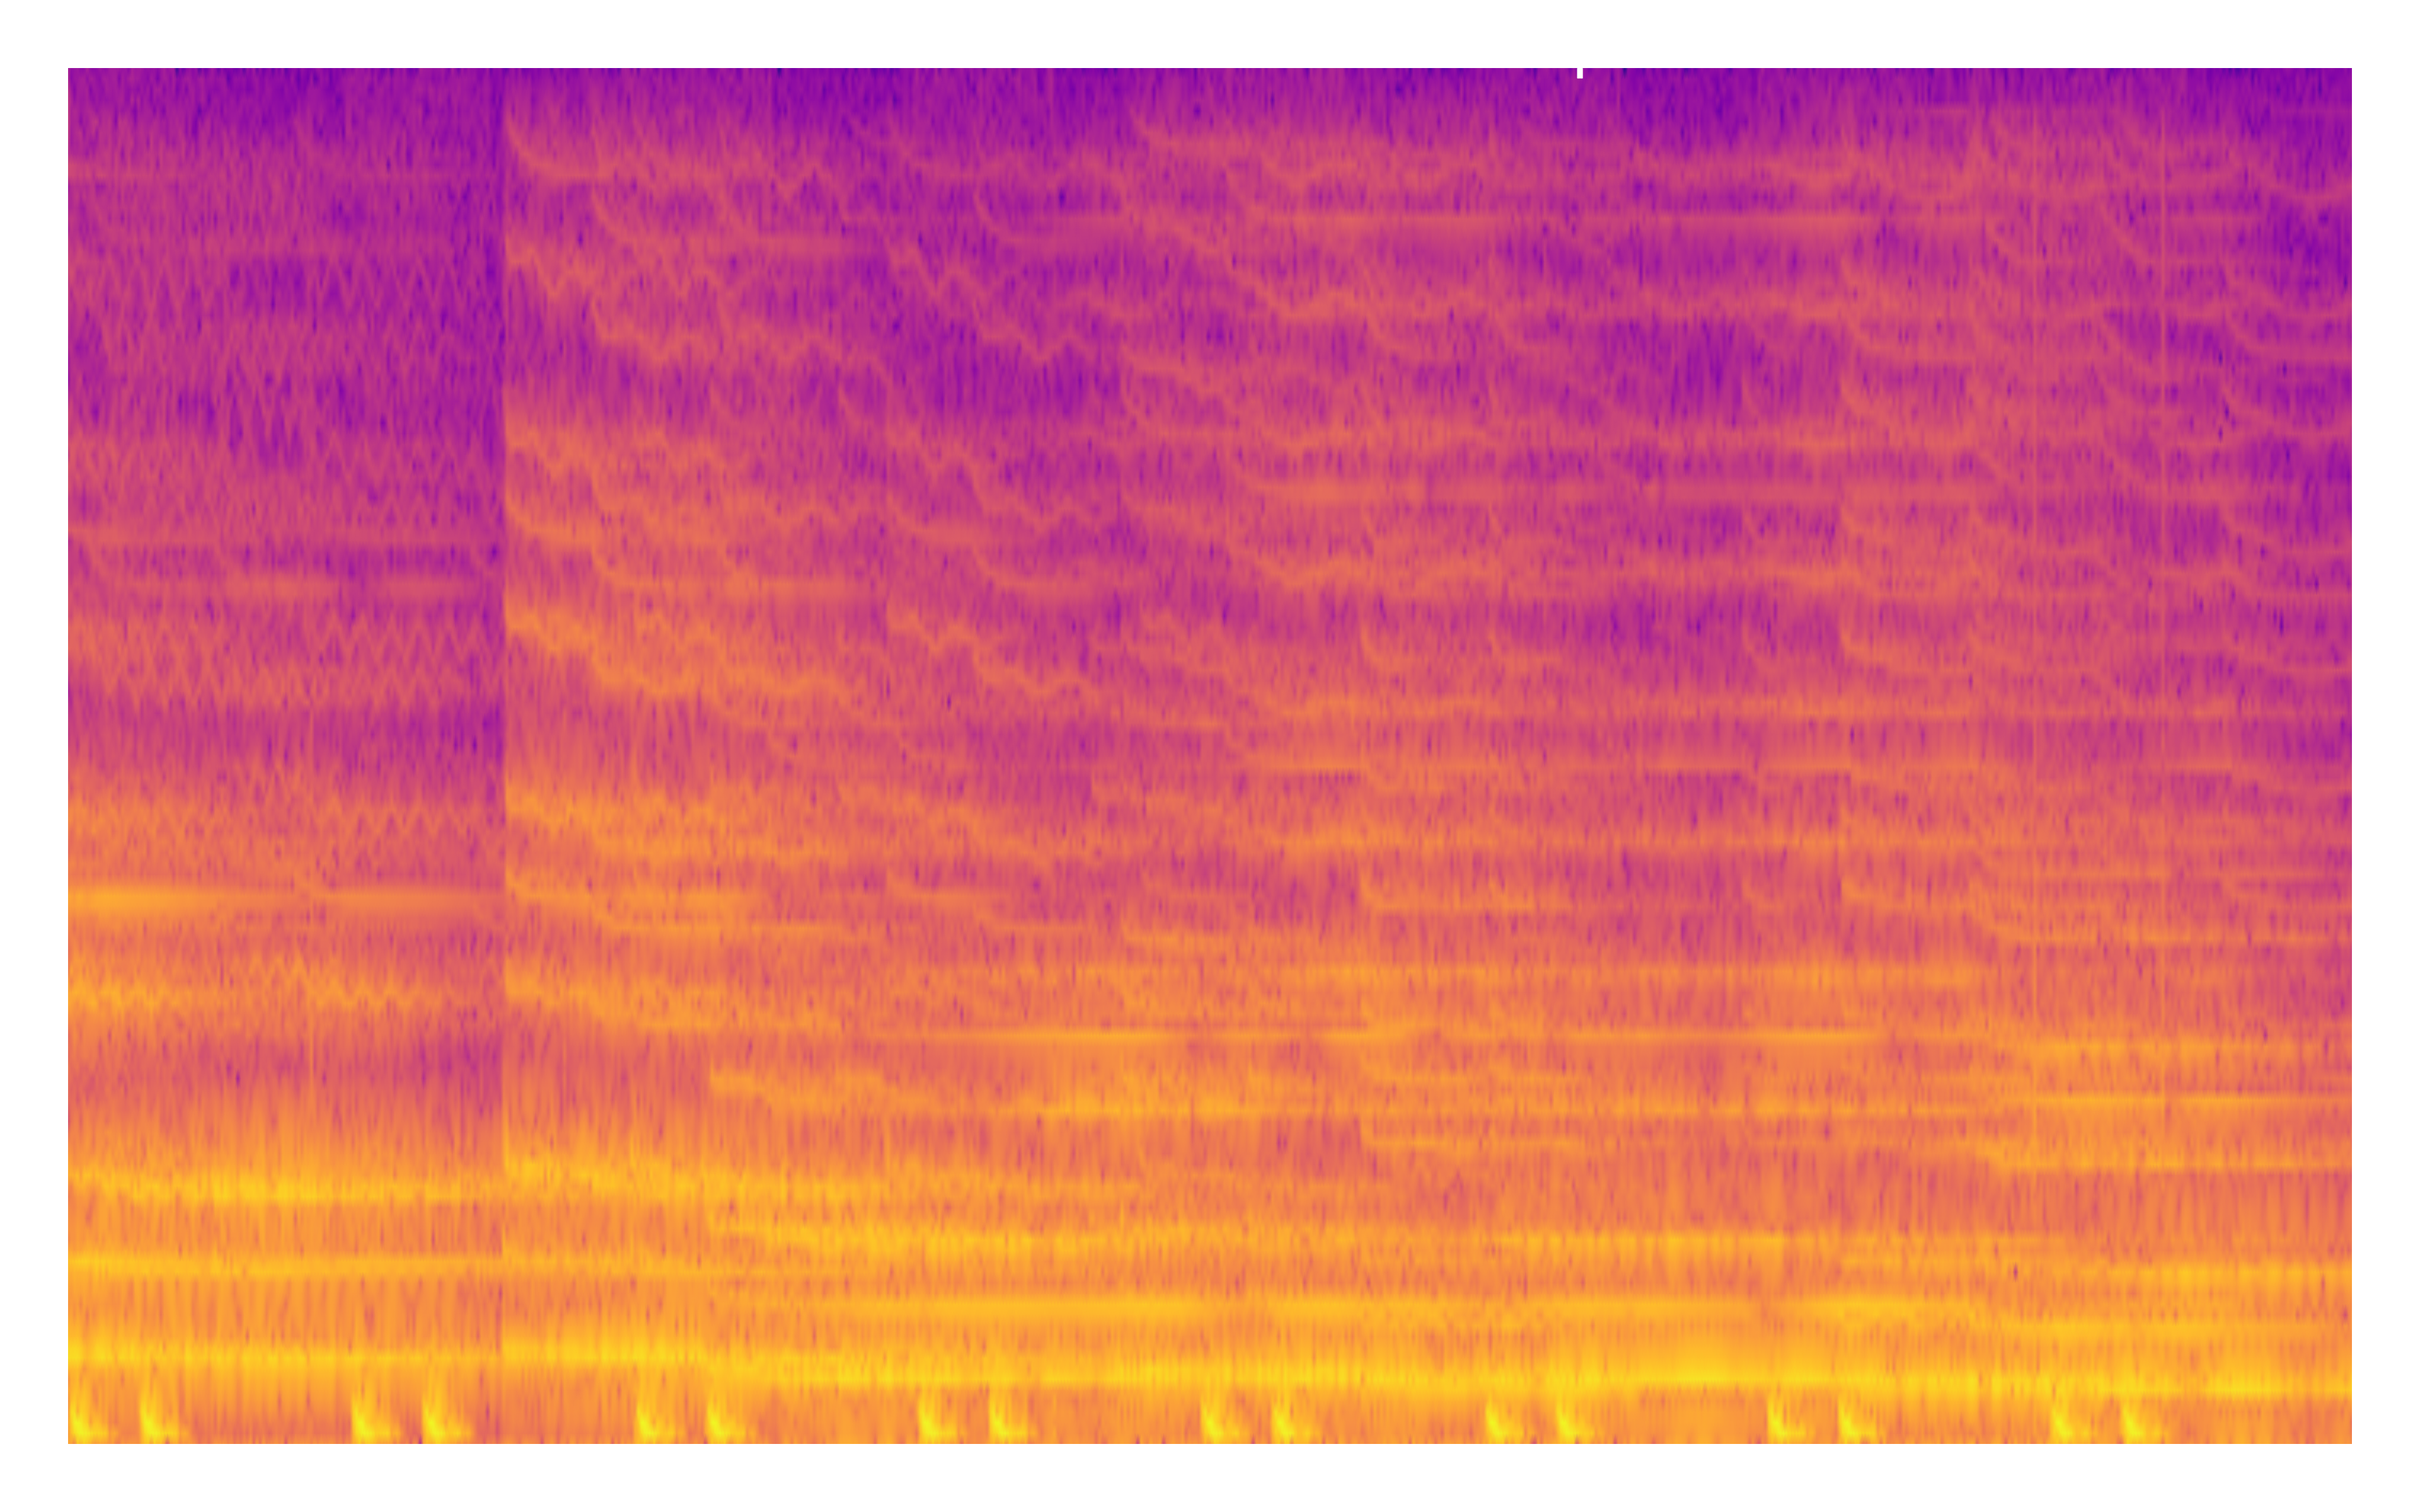
\includegraphics[width=\textwidth]{plots/onepeace_best_sdr/onepeace mixture_spectrogram.png}
    \end{subfigure}
    \begin{subfigure}[b]{0.185\textwidth}
        \centering
        \includegraphics[width=\textwidth]{plots/onepeace_best_sdr/onepeace sep_spectrogram.png}
    \end{subfigure}
    \begin{subfigure}[b]{0.185\textwidth}
        \centering
        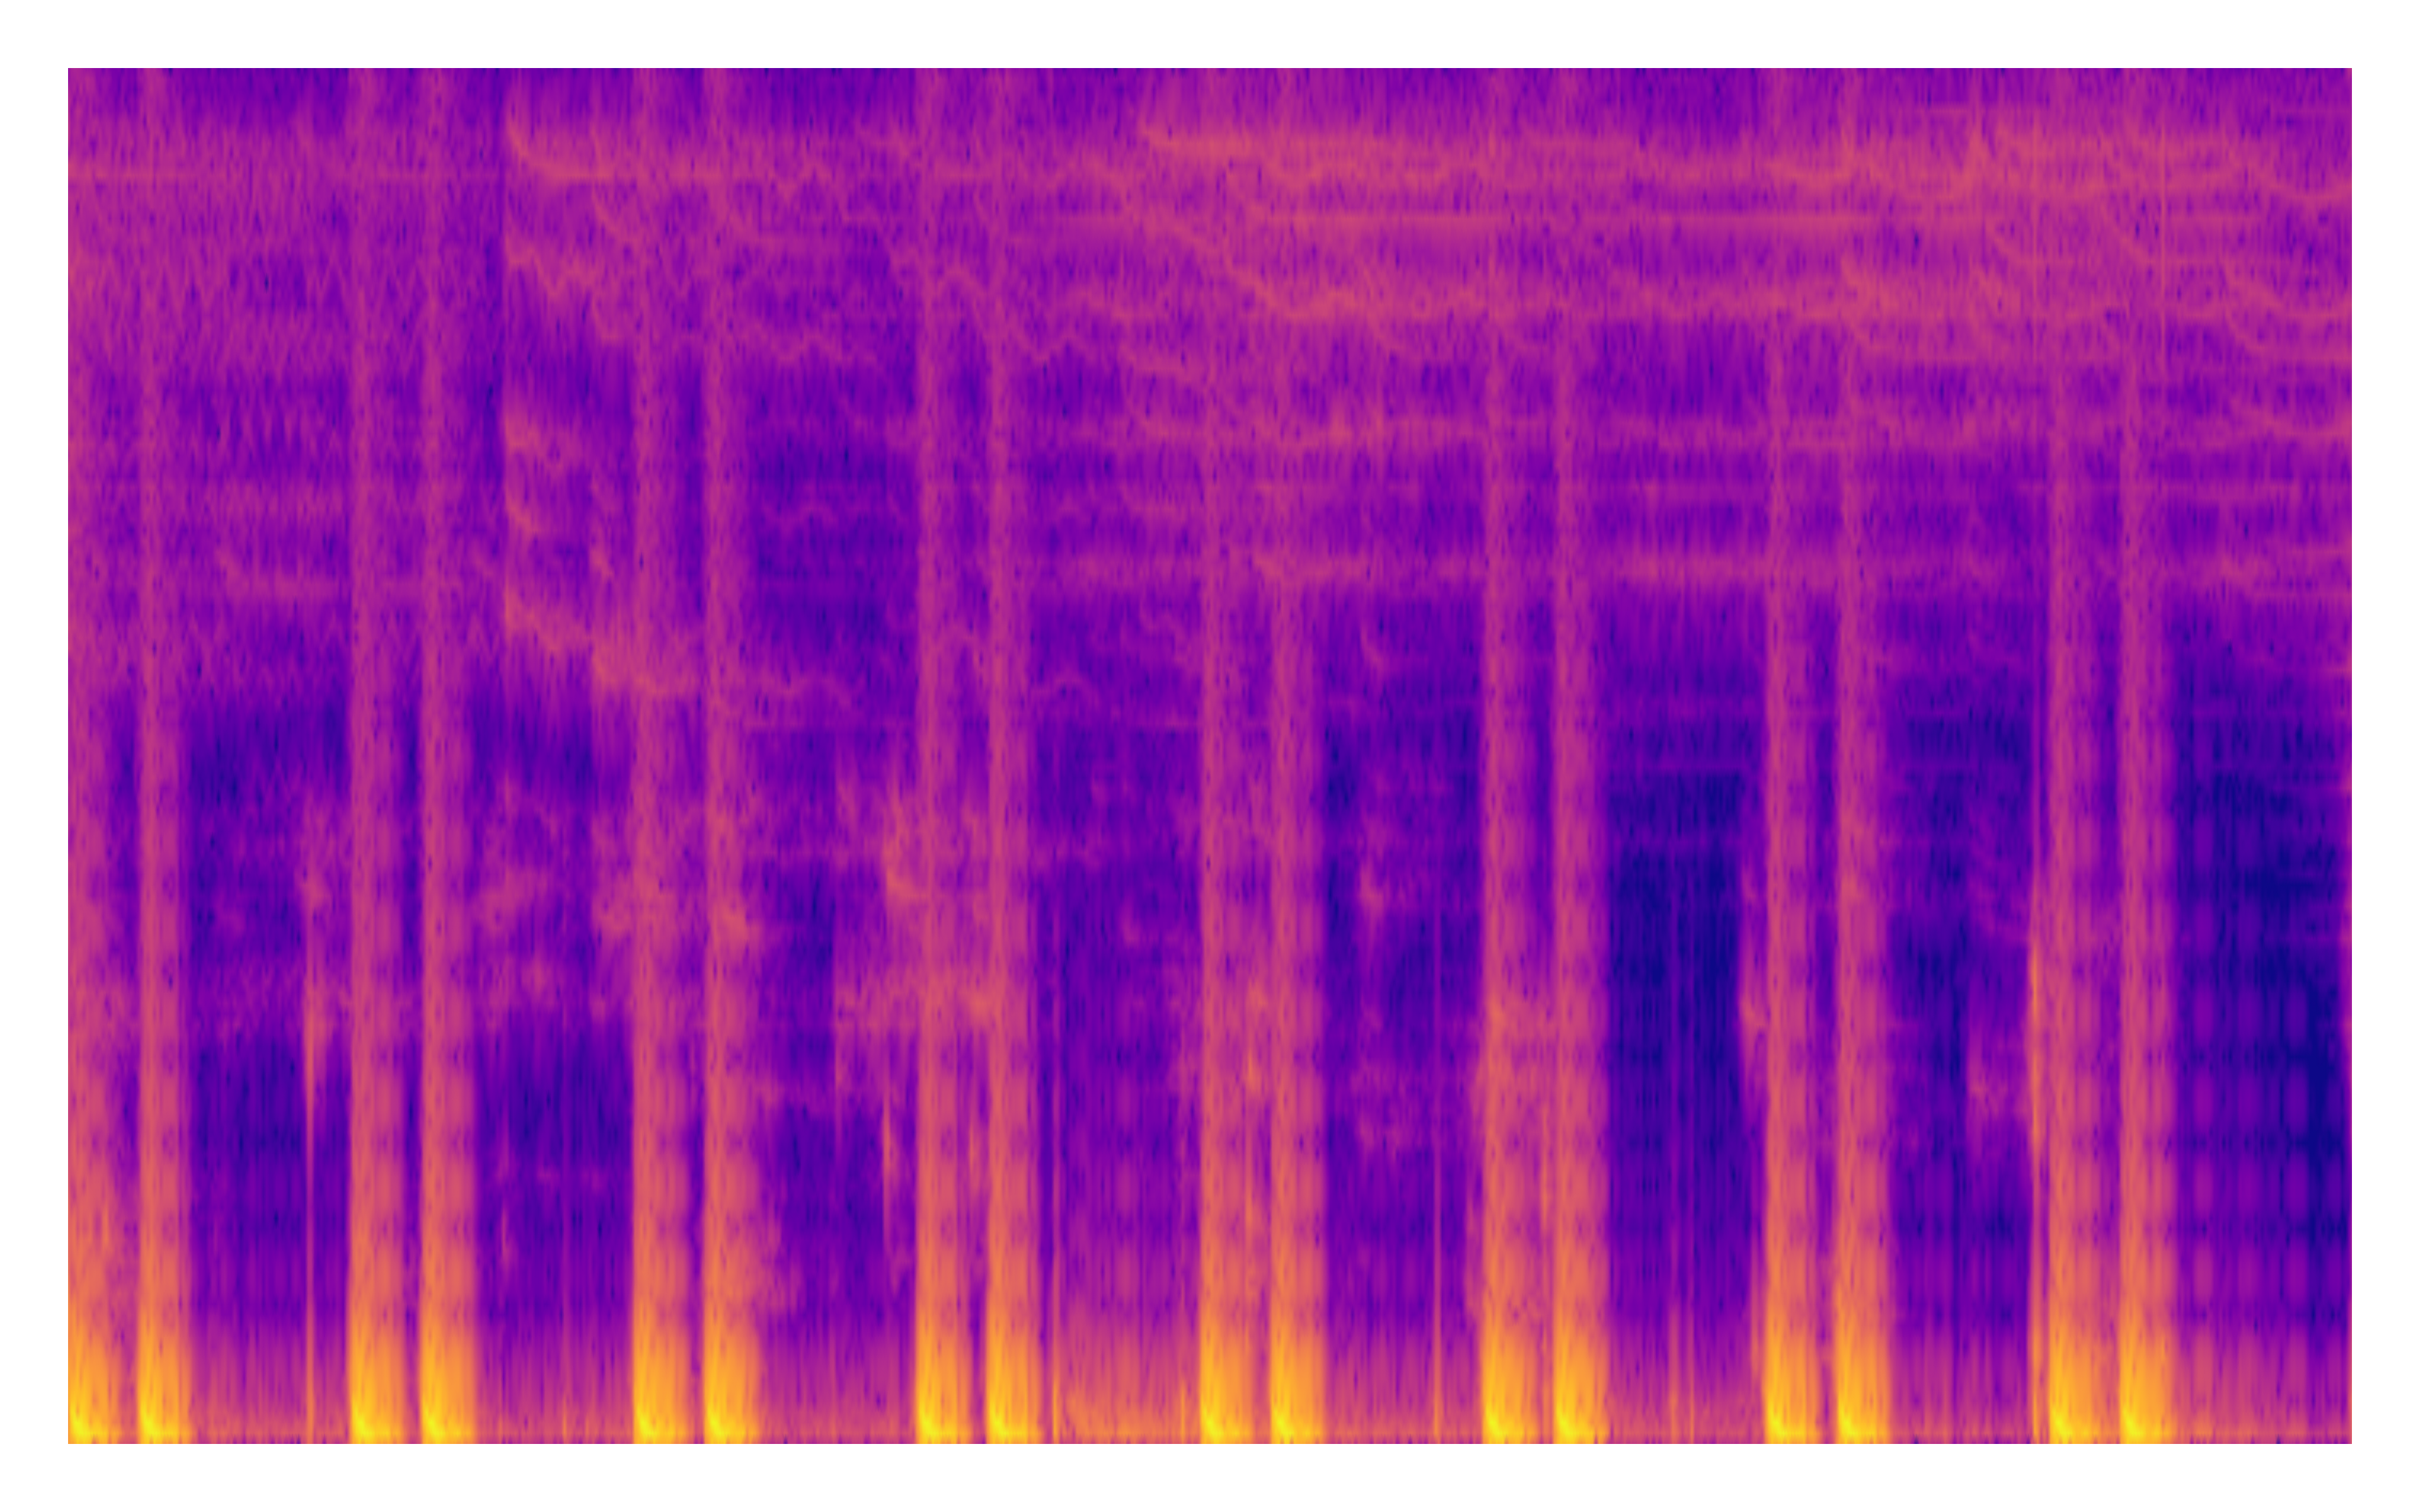
\includegraphics[width=\textwidth]{plots/onepeace_best_sdr/clap sep_spectrogram.png}
    \end{subfigure}
    \begin{subfigure}[b]{0.185\textwidth}
        \centering
        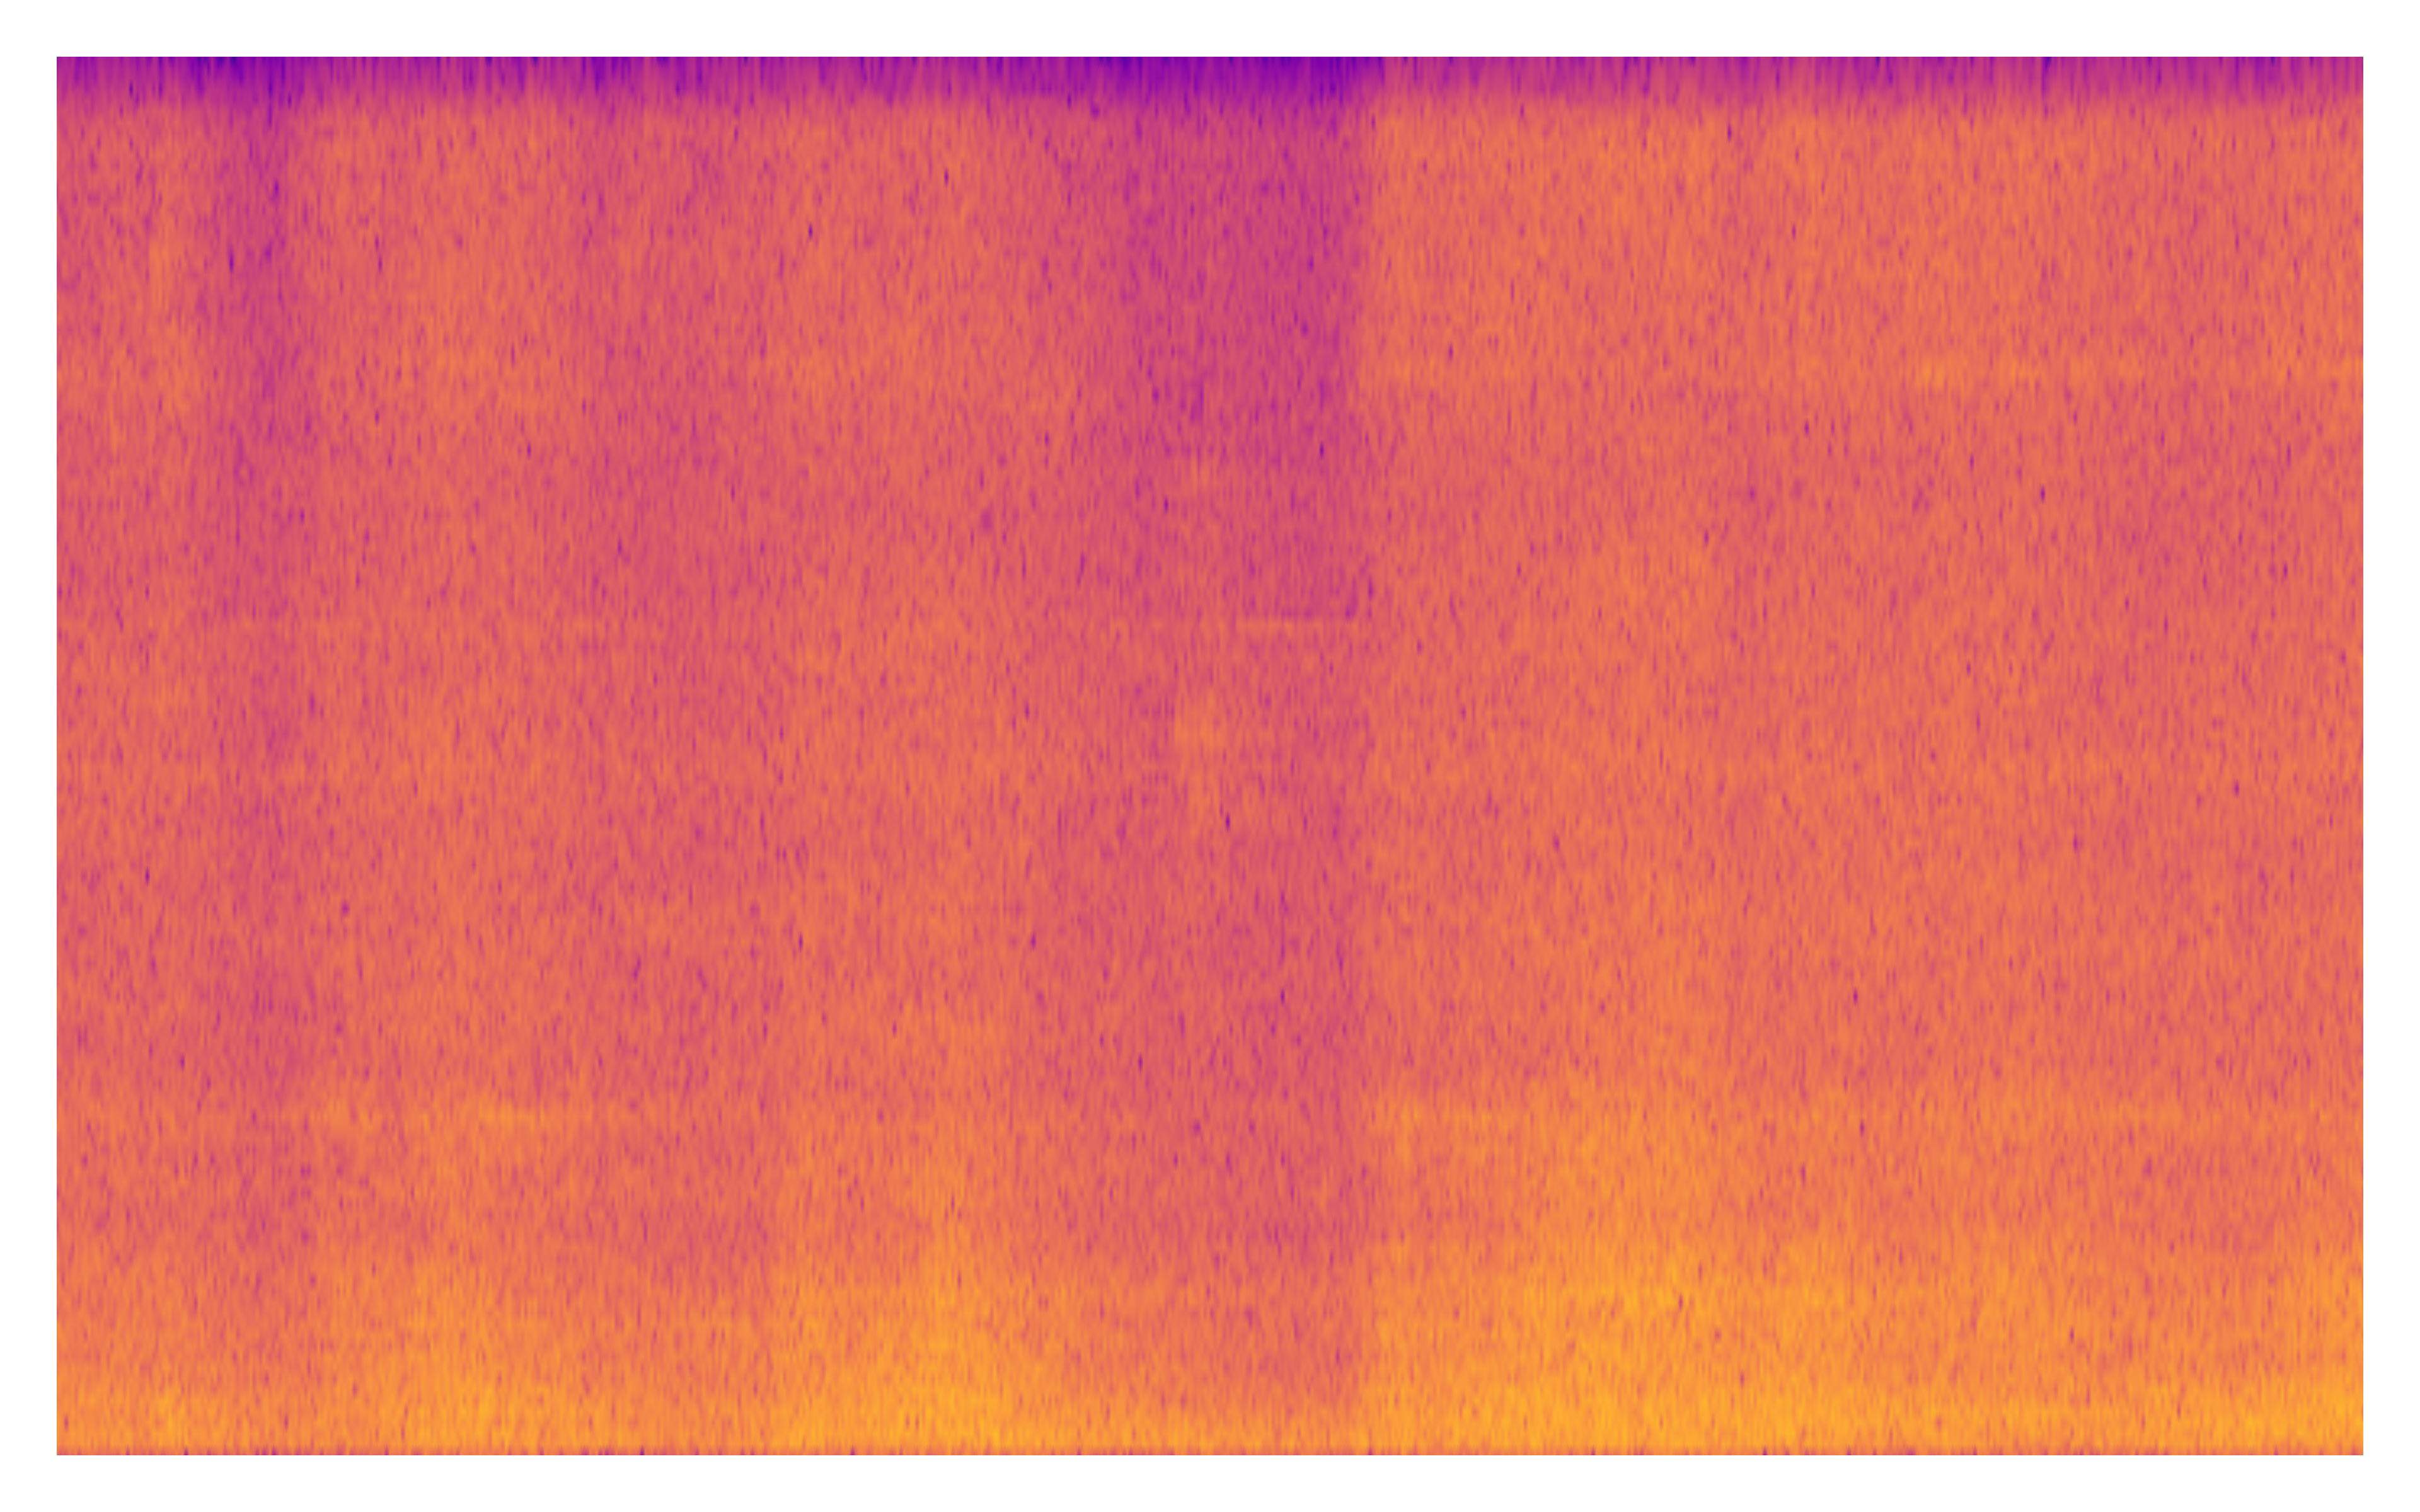
\includegraphics[width=\textwidth]{plots/onepeace_best_sdr/onepeace target_spectrogram.png}
    \end{subfigure}

    % Row 2 Best One-PEACE SDRi
    \begin{subfigure}[b]{0.185\textwidth}
        \centering
        \scriptsize\textbf{"Someone is shoveling something, making a clinking sound"}
        \vspace{5.0mm}
    \end{subfigure}
    \begin{subfigure}[b]{0.185\textwidth}
        \centering
        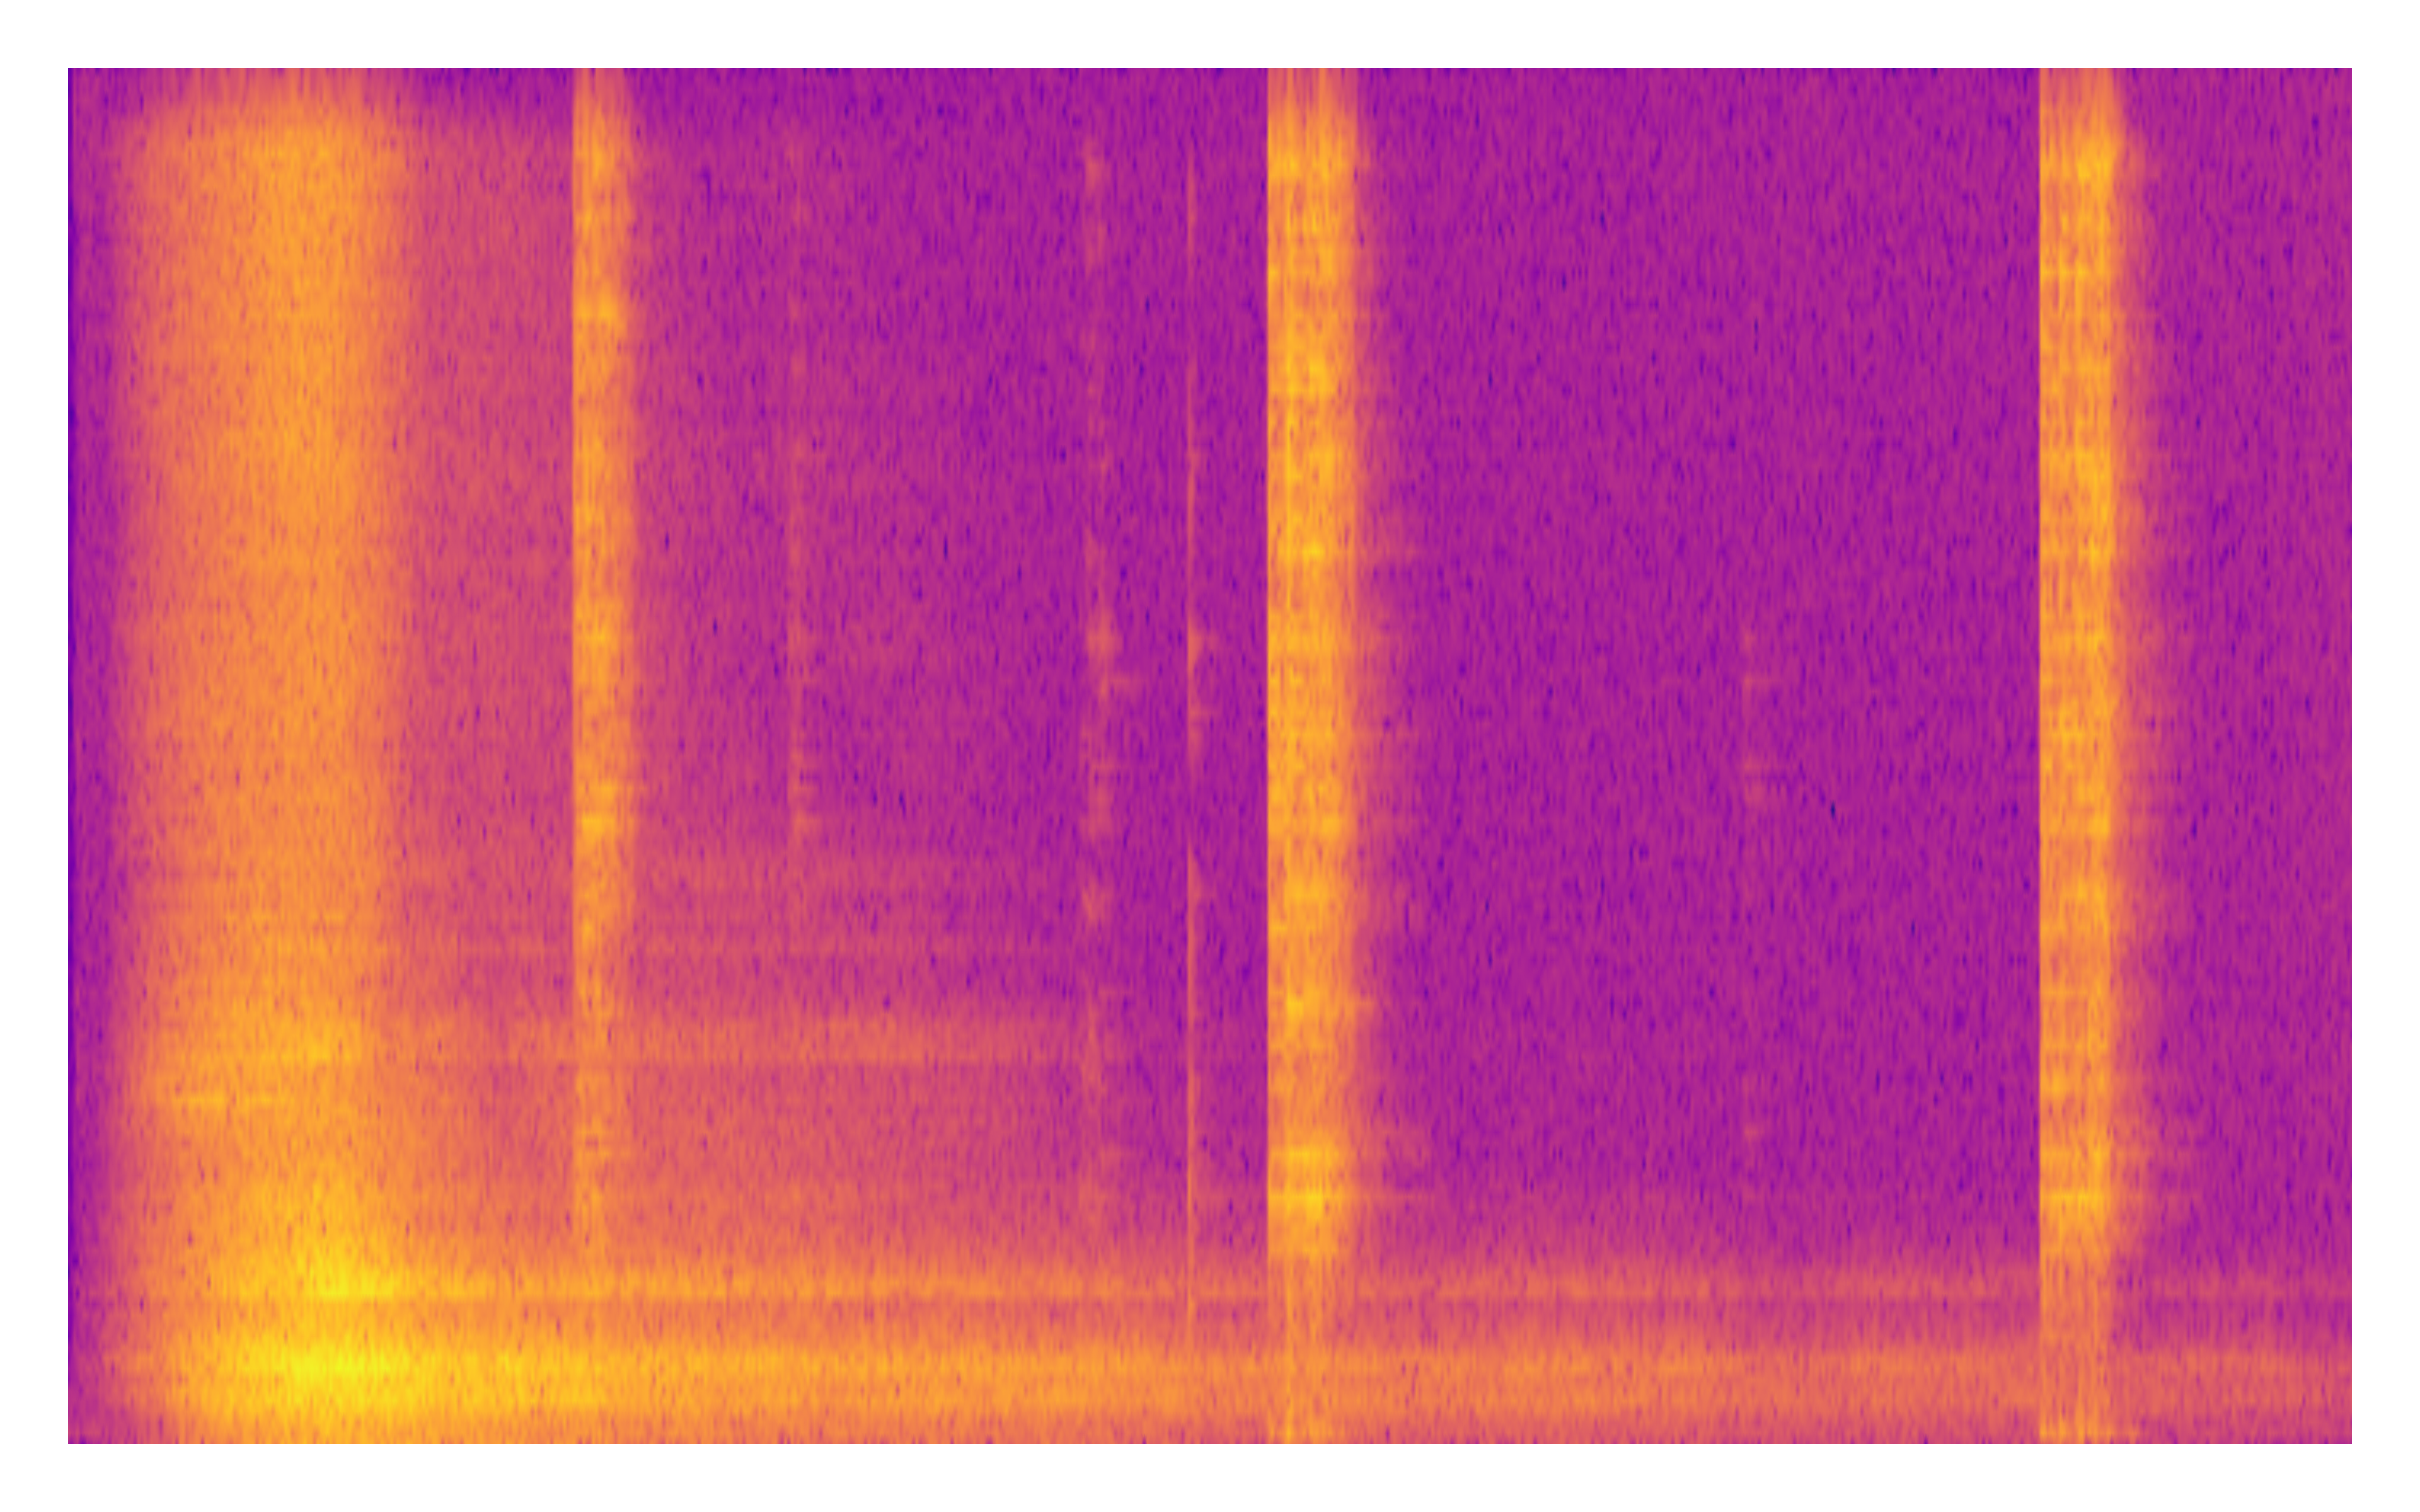
\includegraphics[width=\textwidth]{plots/onepeace_best_sdri/onepeace mixture_spectrogram.png}
    \end{subfigure}
    \begin{subfigure}[b]{0.185\textwidth}
        \centering
        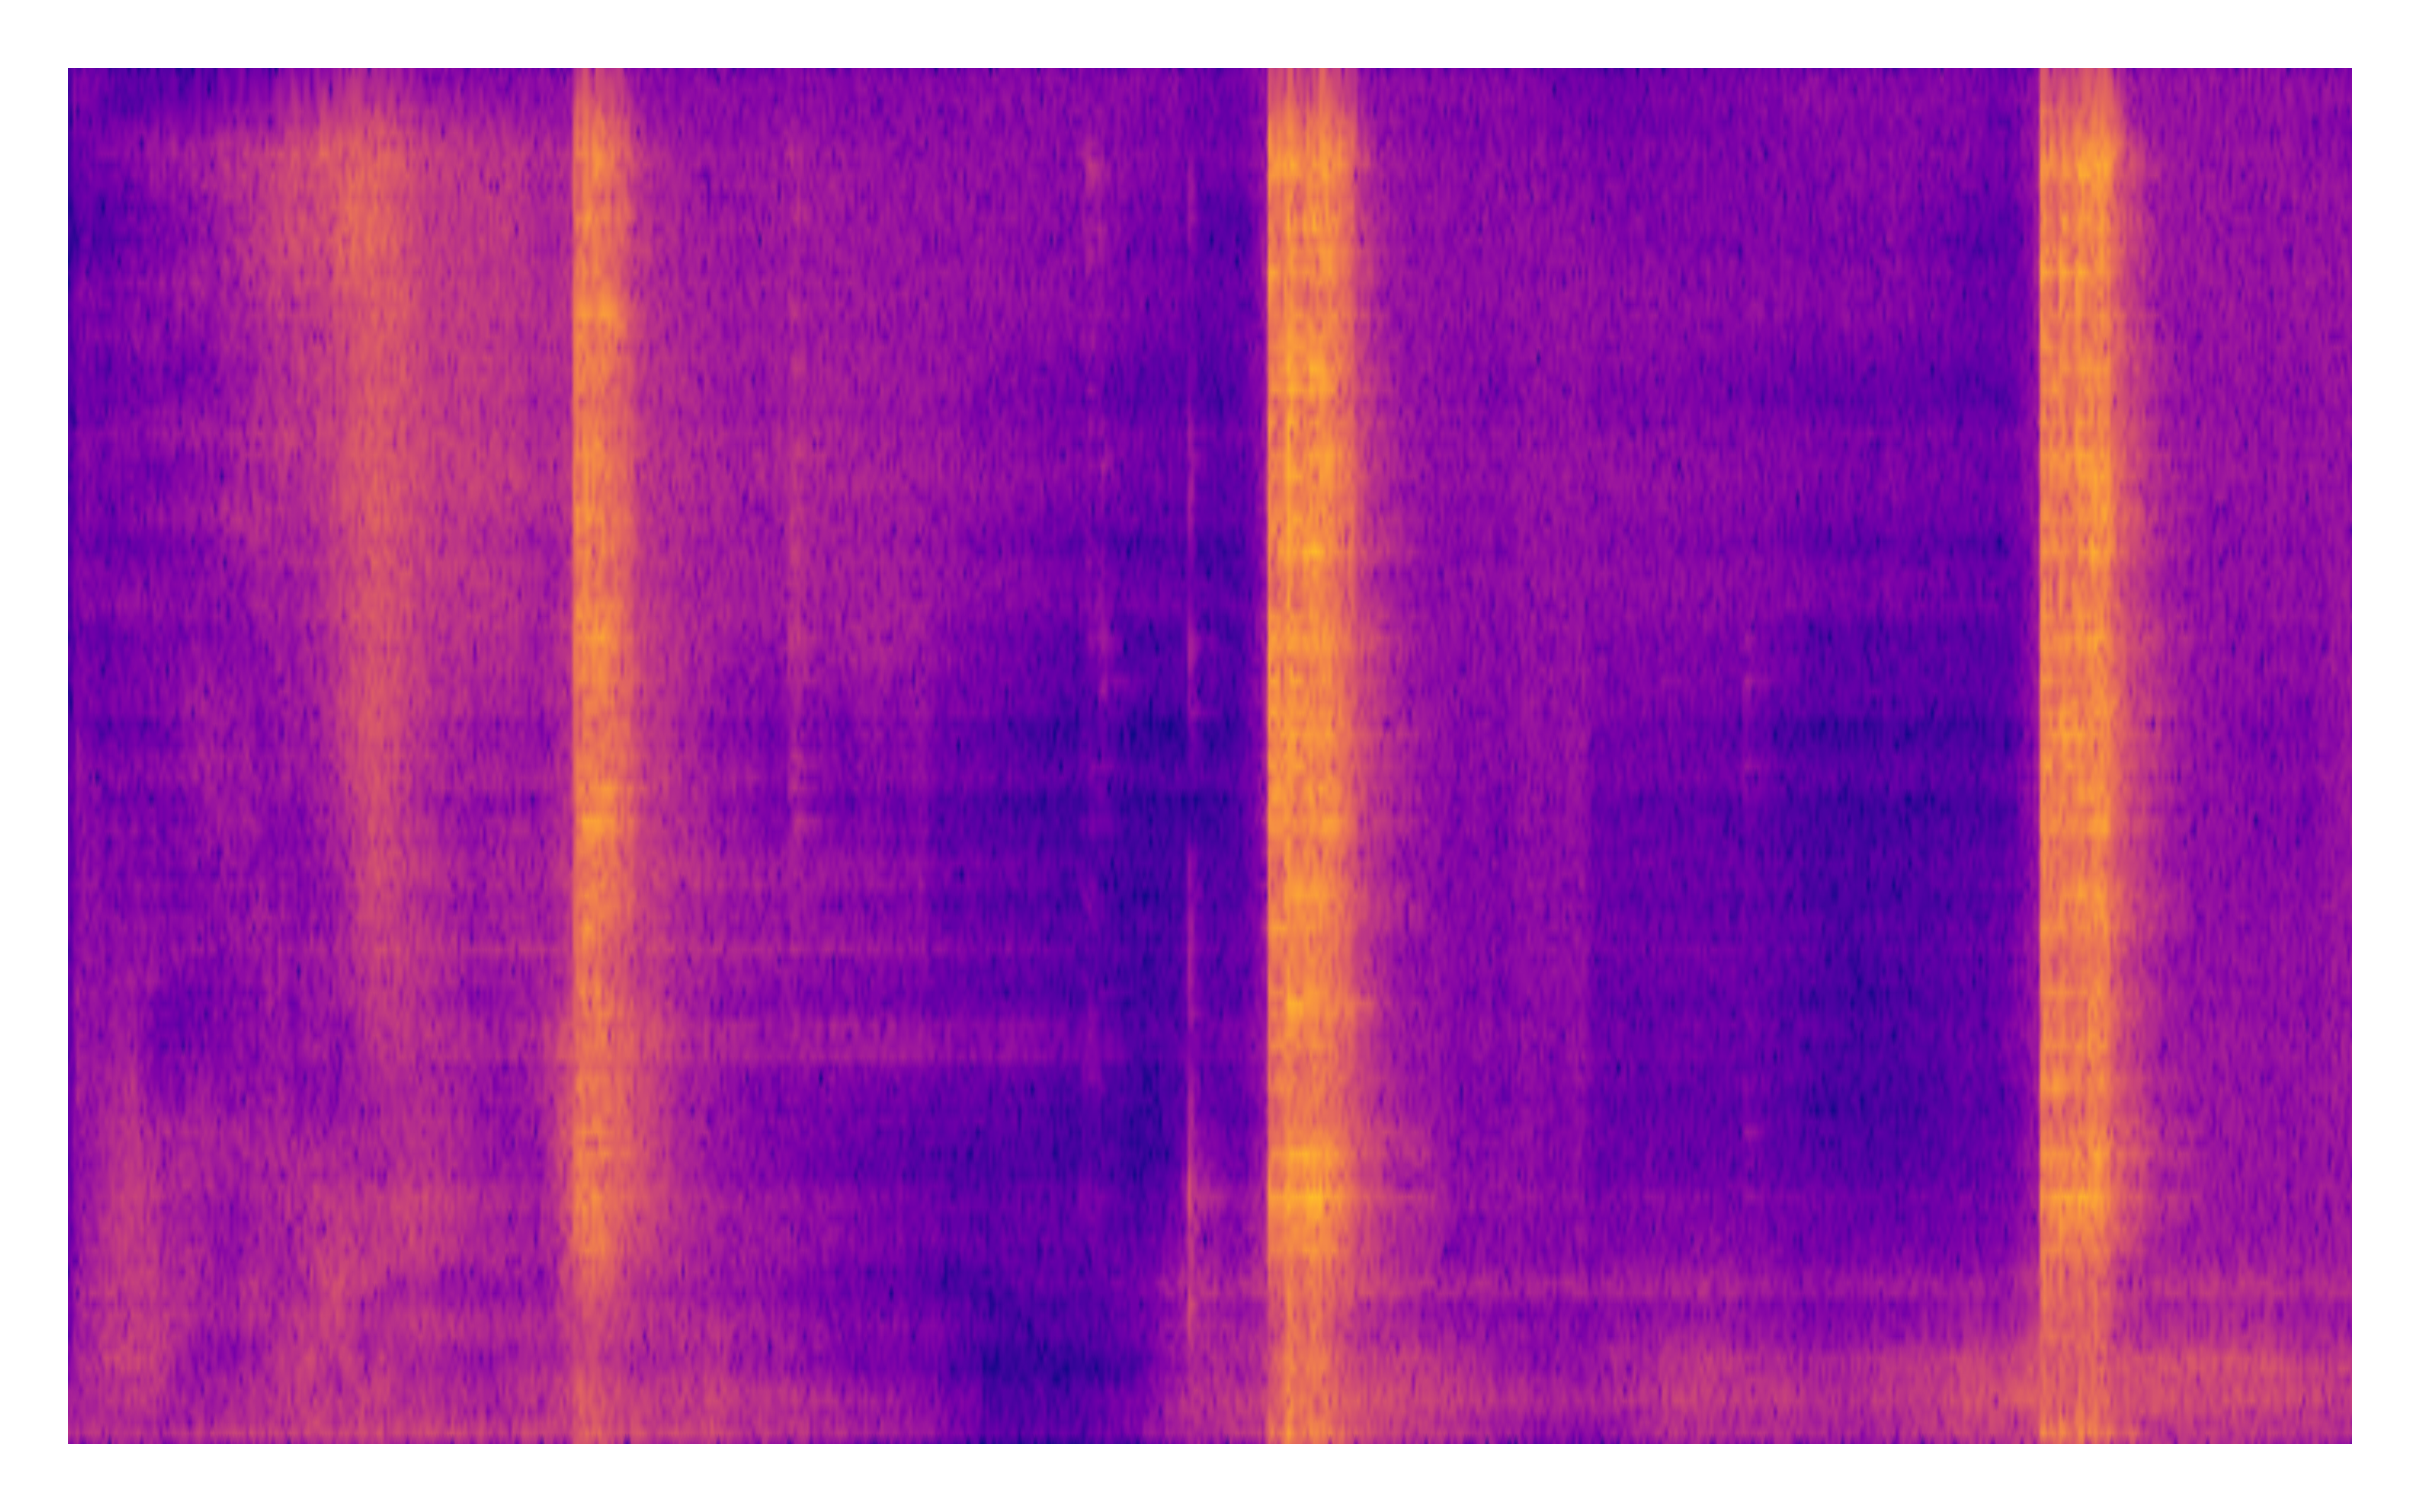
\includegraphics[width=\textwidth]{plots/onepeace_best_sdri/onepeace sep_spectrogram.png}
    \end{subfigure}
    \begin{subfigure}[b]{0.185\textwidth}
        \centering
        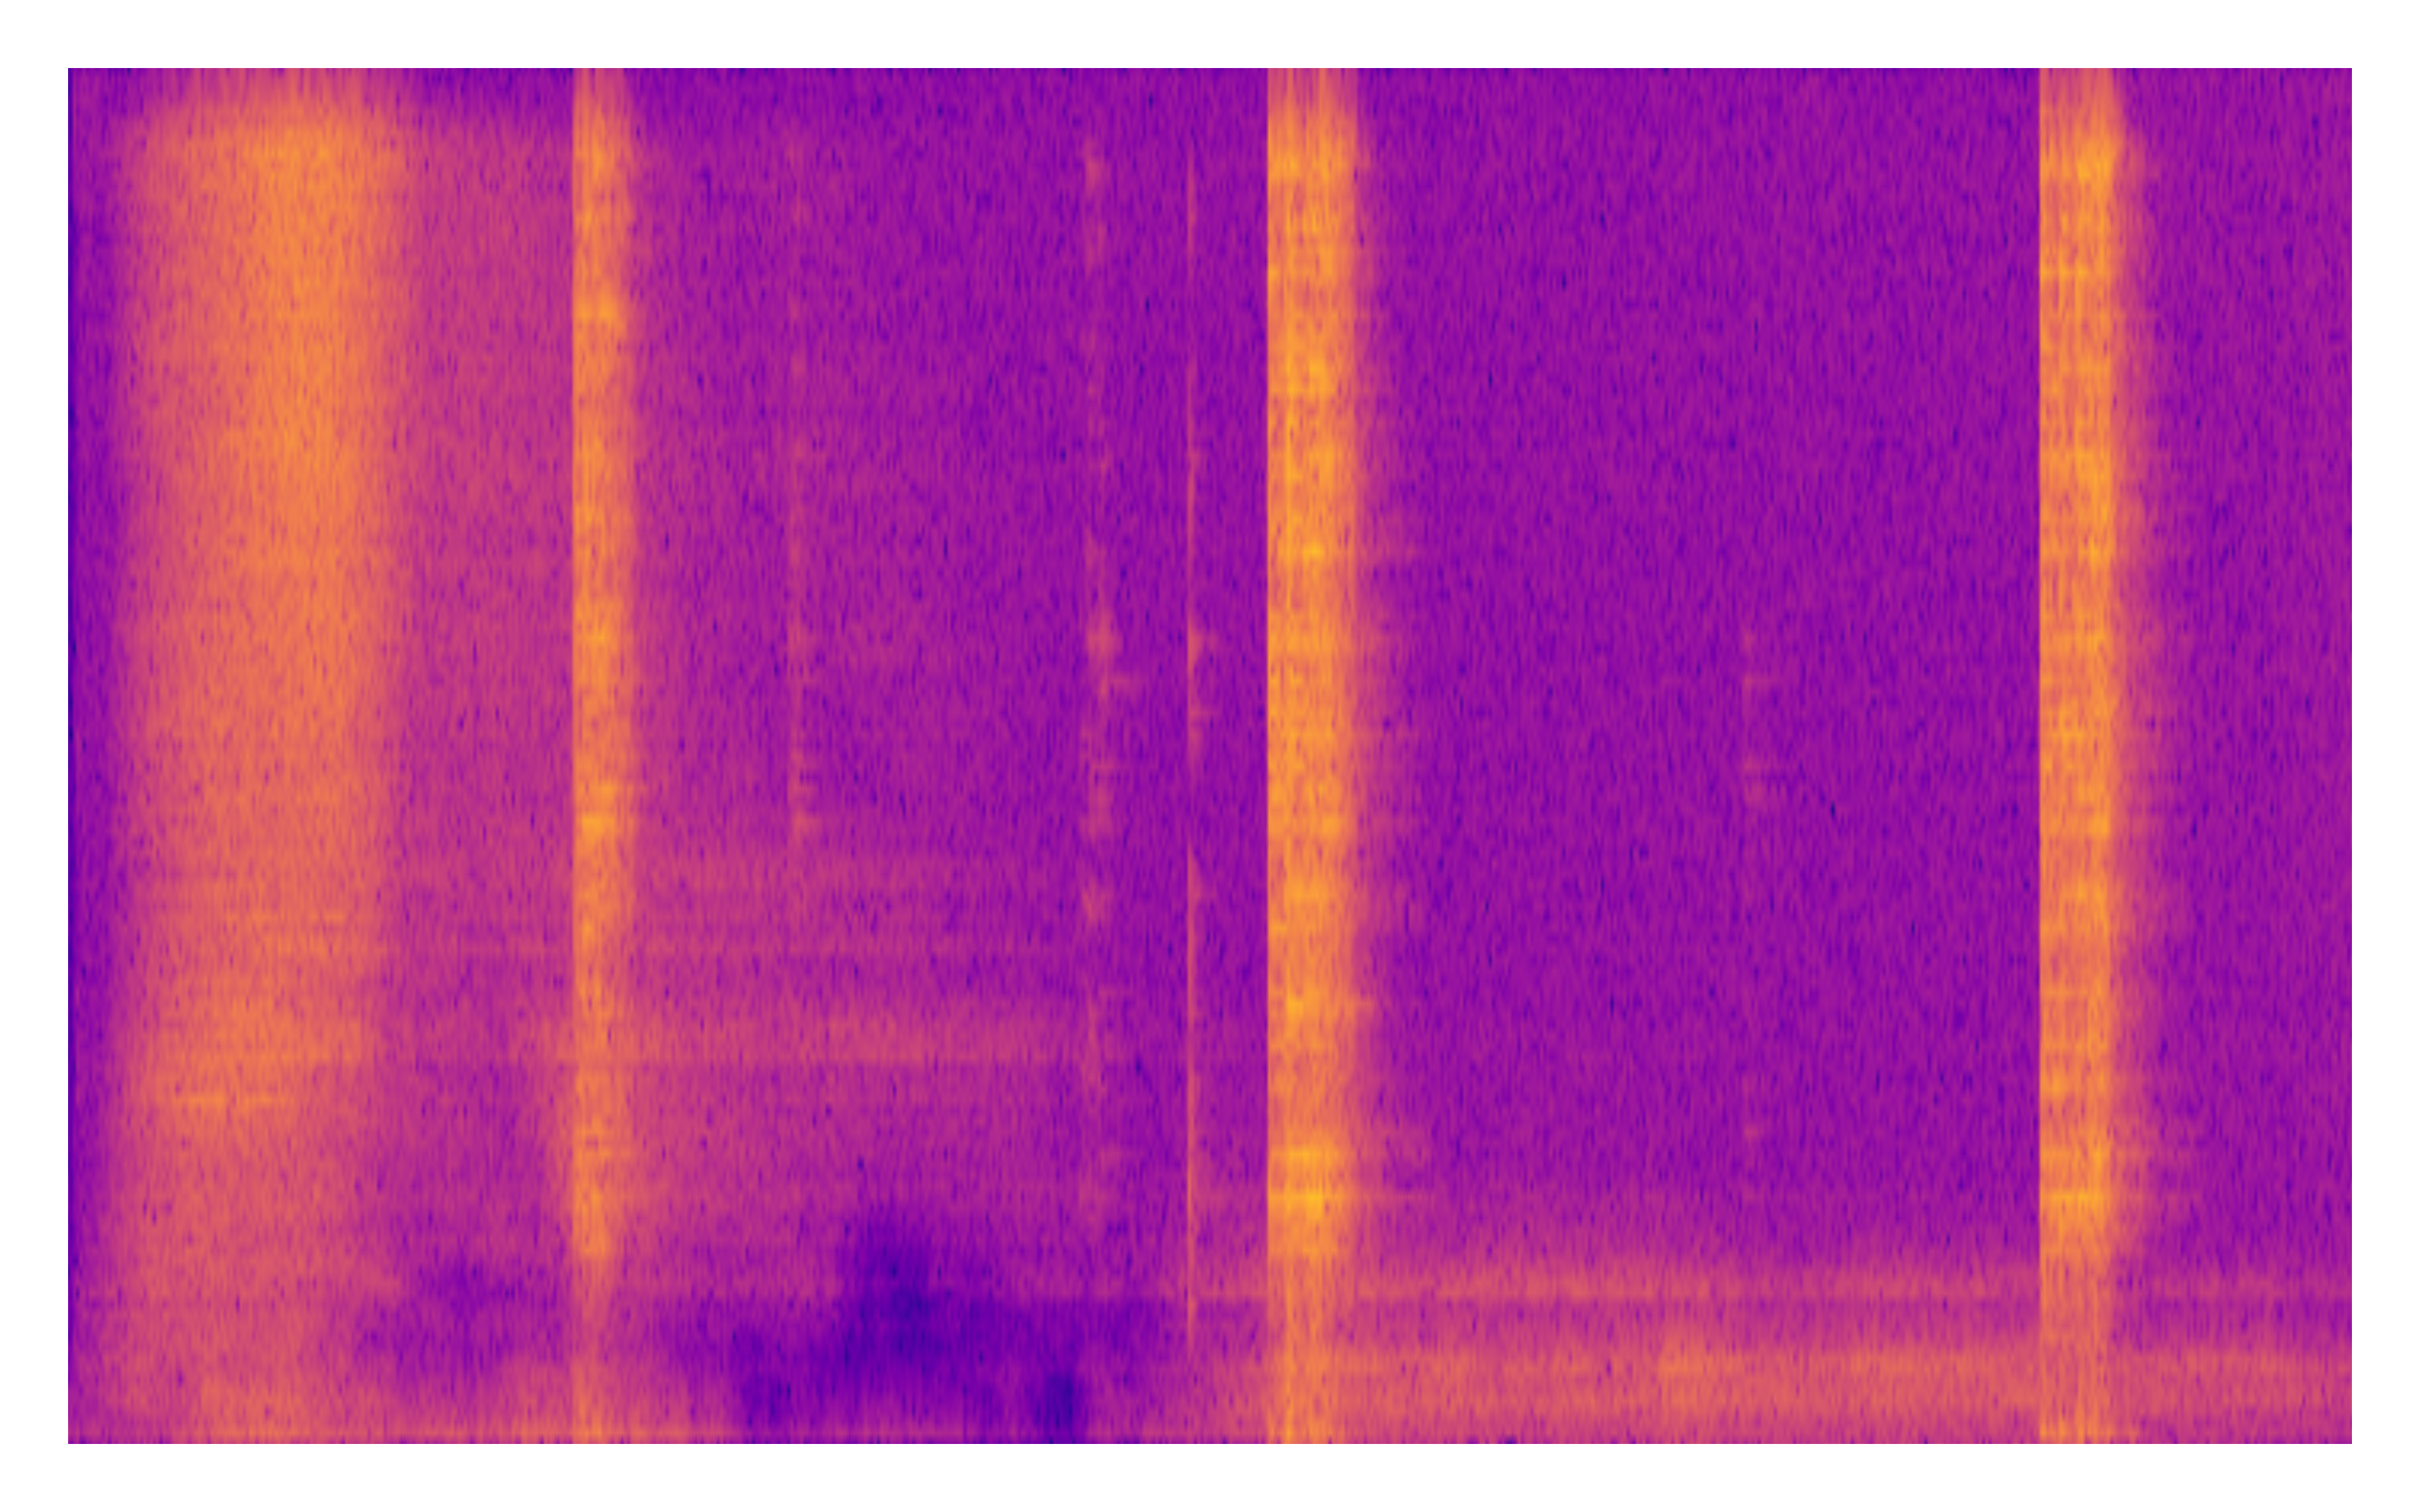
\includegraphics[width=\textwidth]{plots/onepeace_best_sdri/clap sep_spectrogram.png}
    \end{subfigure}
    \begin{subfigure}[b]{0.185\textwidth}
        \centering
        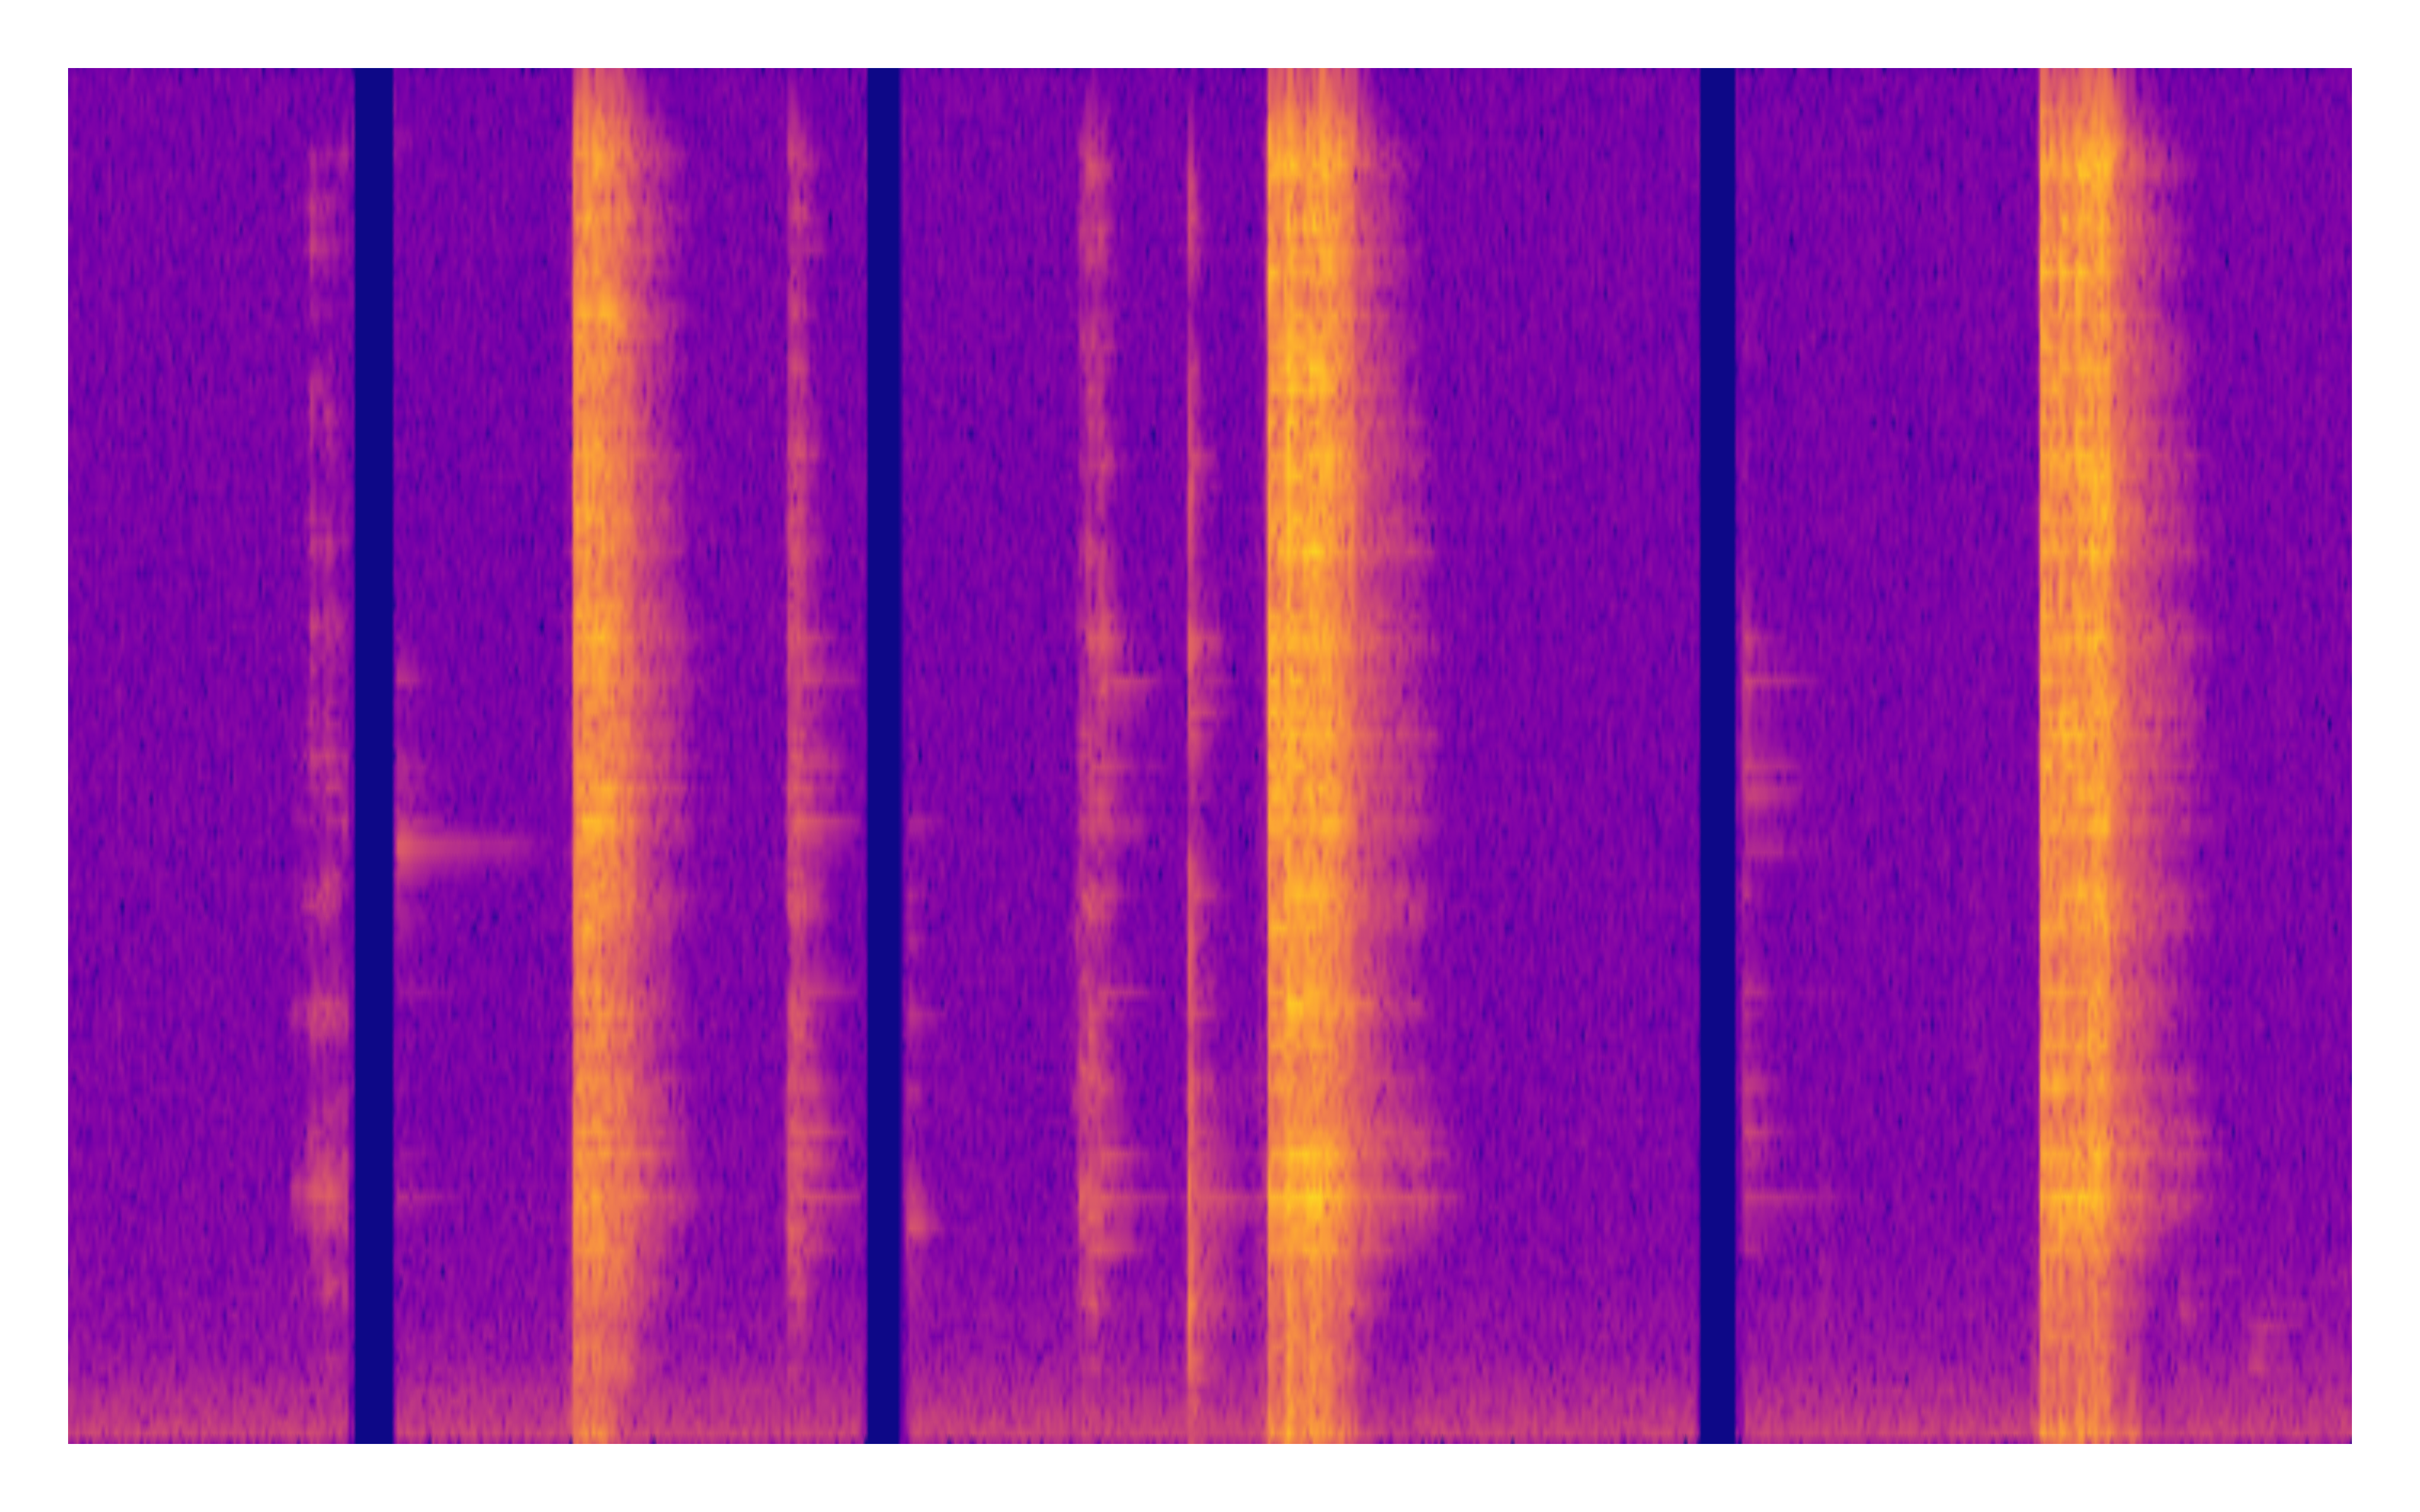
\includegraphics[width=\textwidth]{plots/onepeace_best_sdri/onepeace target_spectrogram.png}
    \end{subfigure}

    % Row 3 best onepeace delta_similarity improvement
     \begin{subfigure}[b]{0.185\textwidth}
        \centering
        \scriptsize\textbf{"Fireworks are shot into the air with swirling sounds and then they explode"}
        \vspace{5.0mm}
    \end{subfigure}
    \begin{subfigure}[b]{0.185\textwidth}
        \centering
        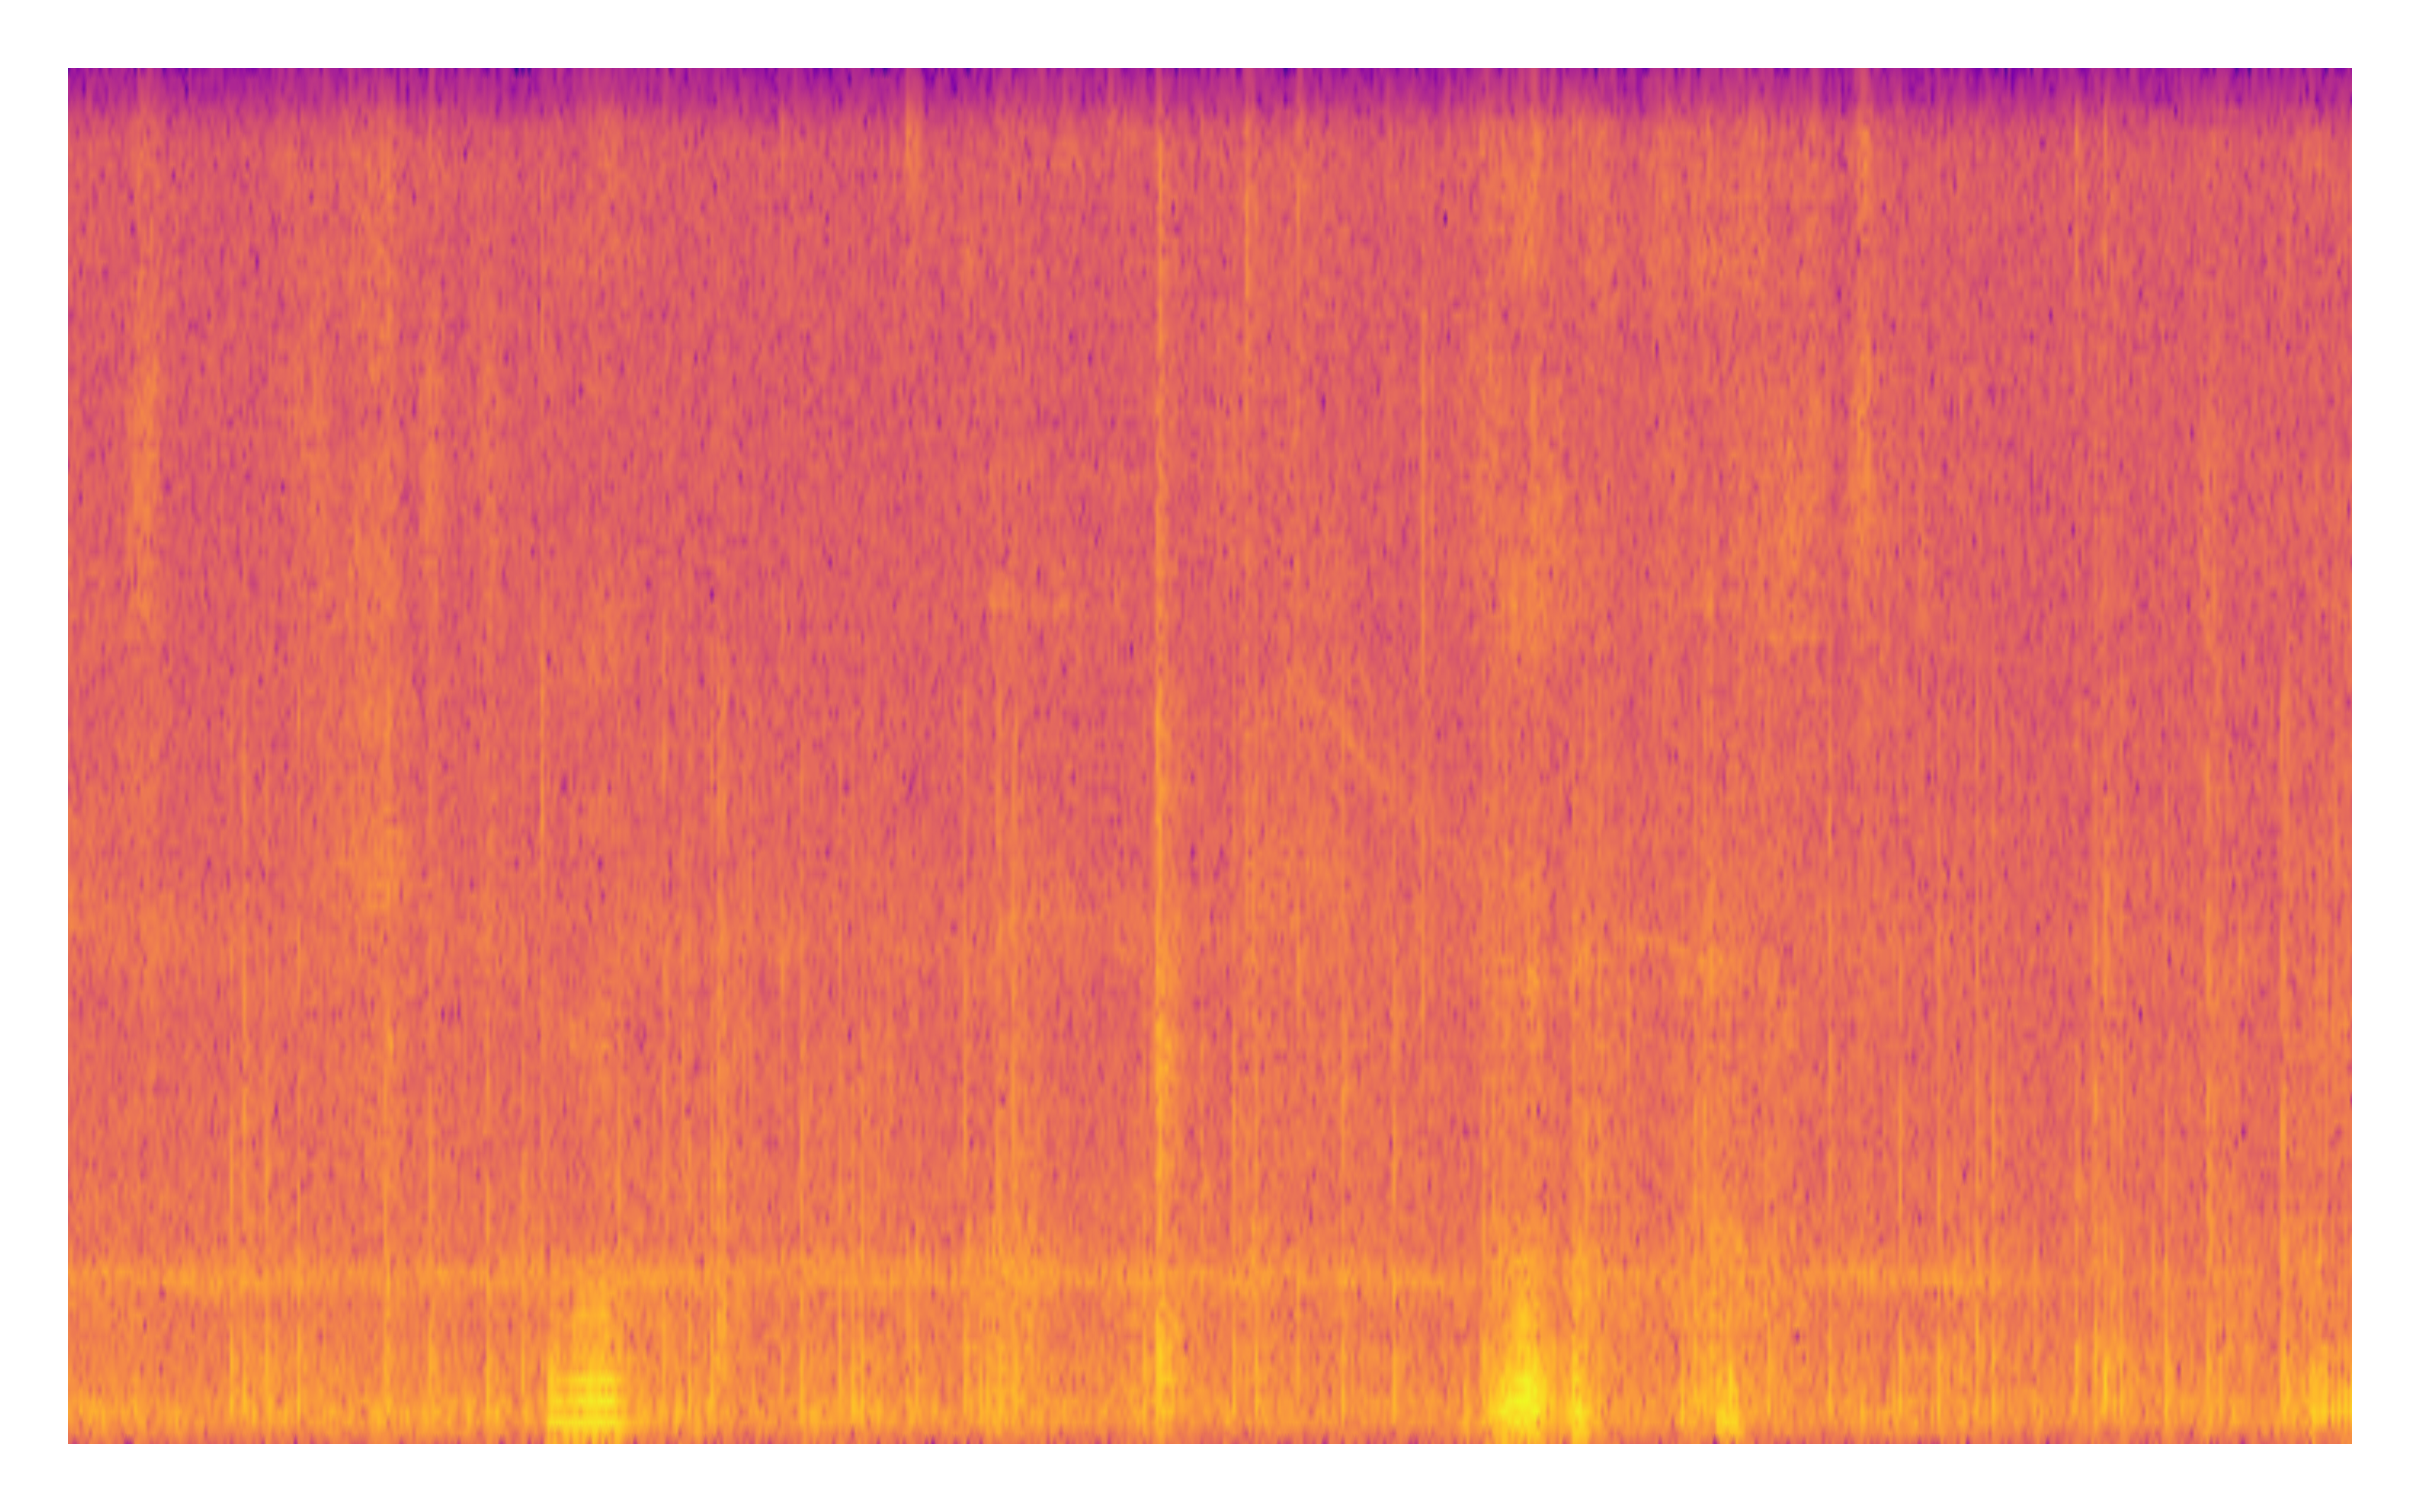
\includegraphics[width=\textwidth]{plots/onepeace_best_delta_similarity/onepeace mixture_spectrogram.png}
    \end{subfigure}
    \begin{subfigure}[b]{0.185\textwidth}
        \centering
        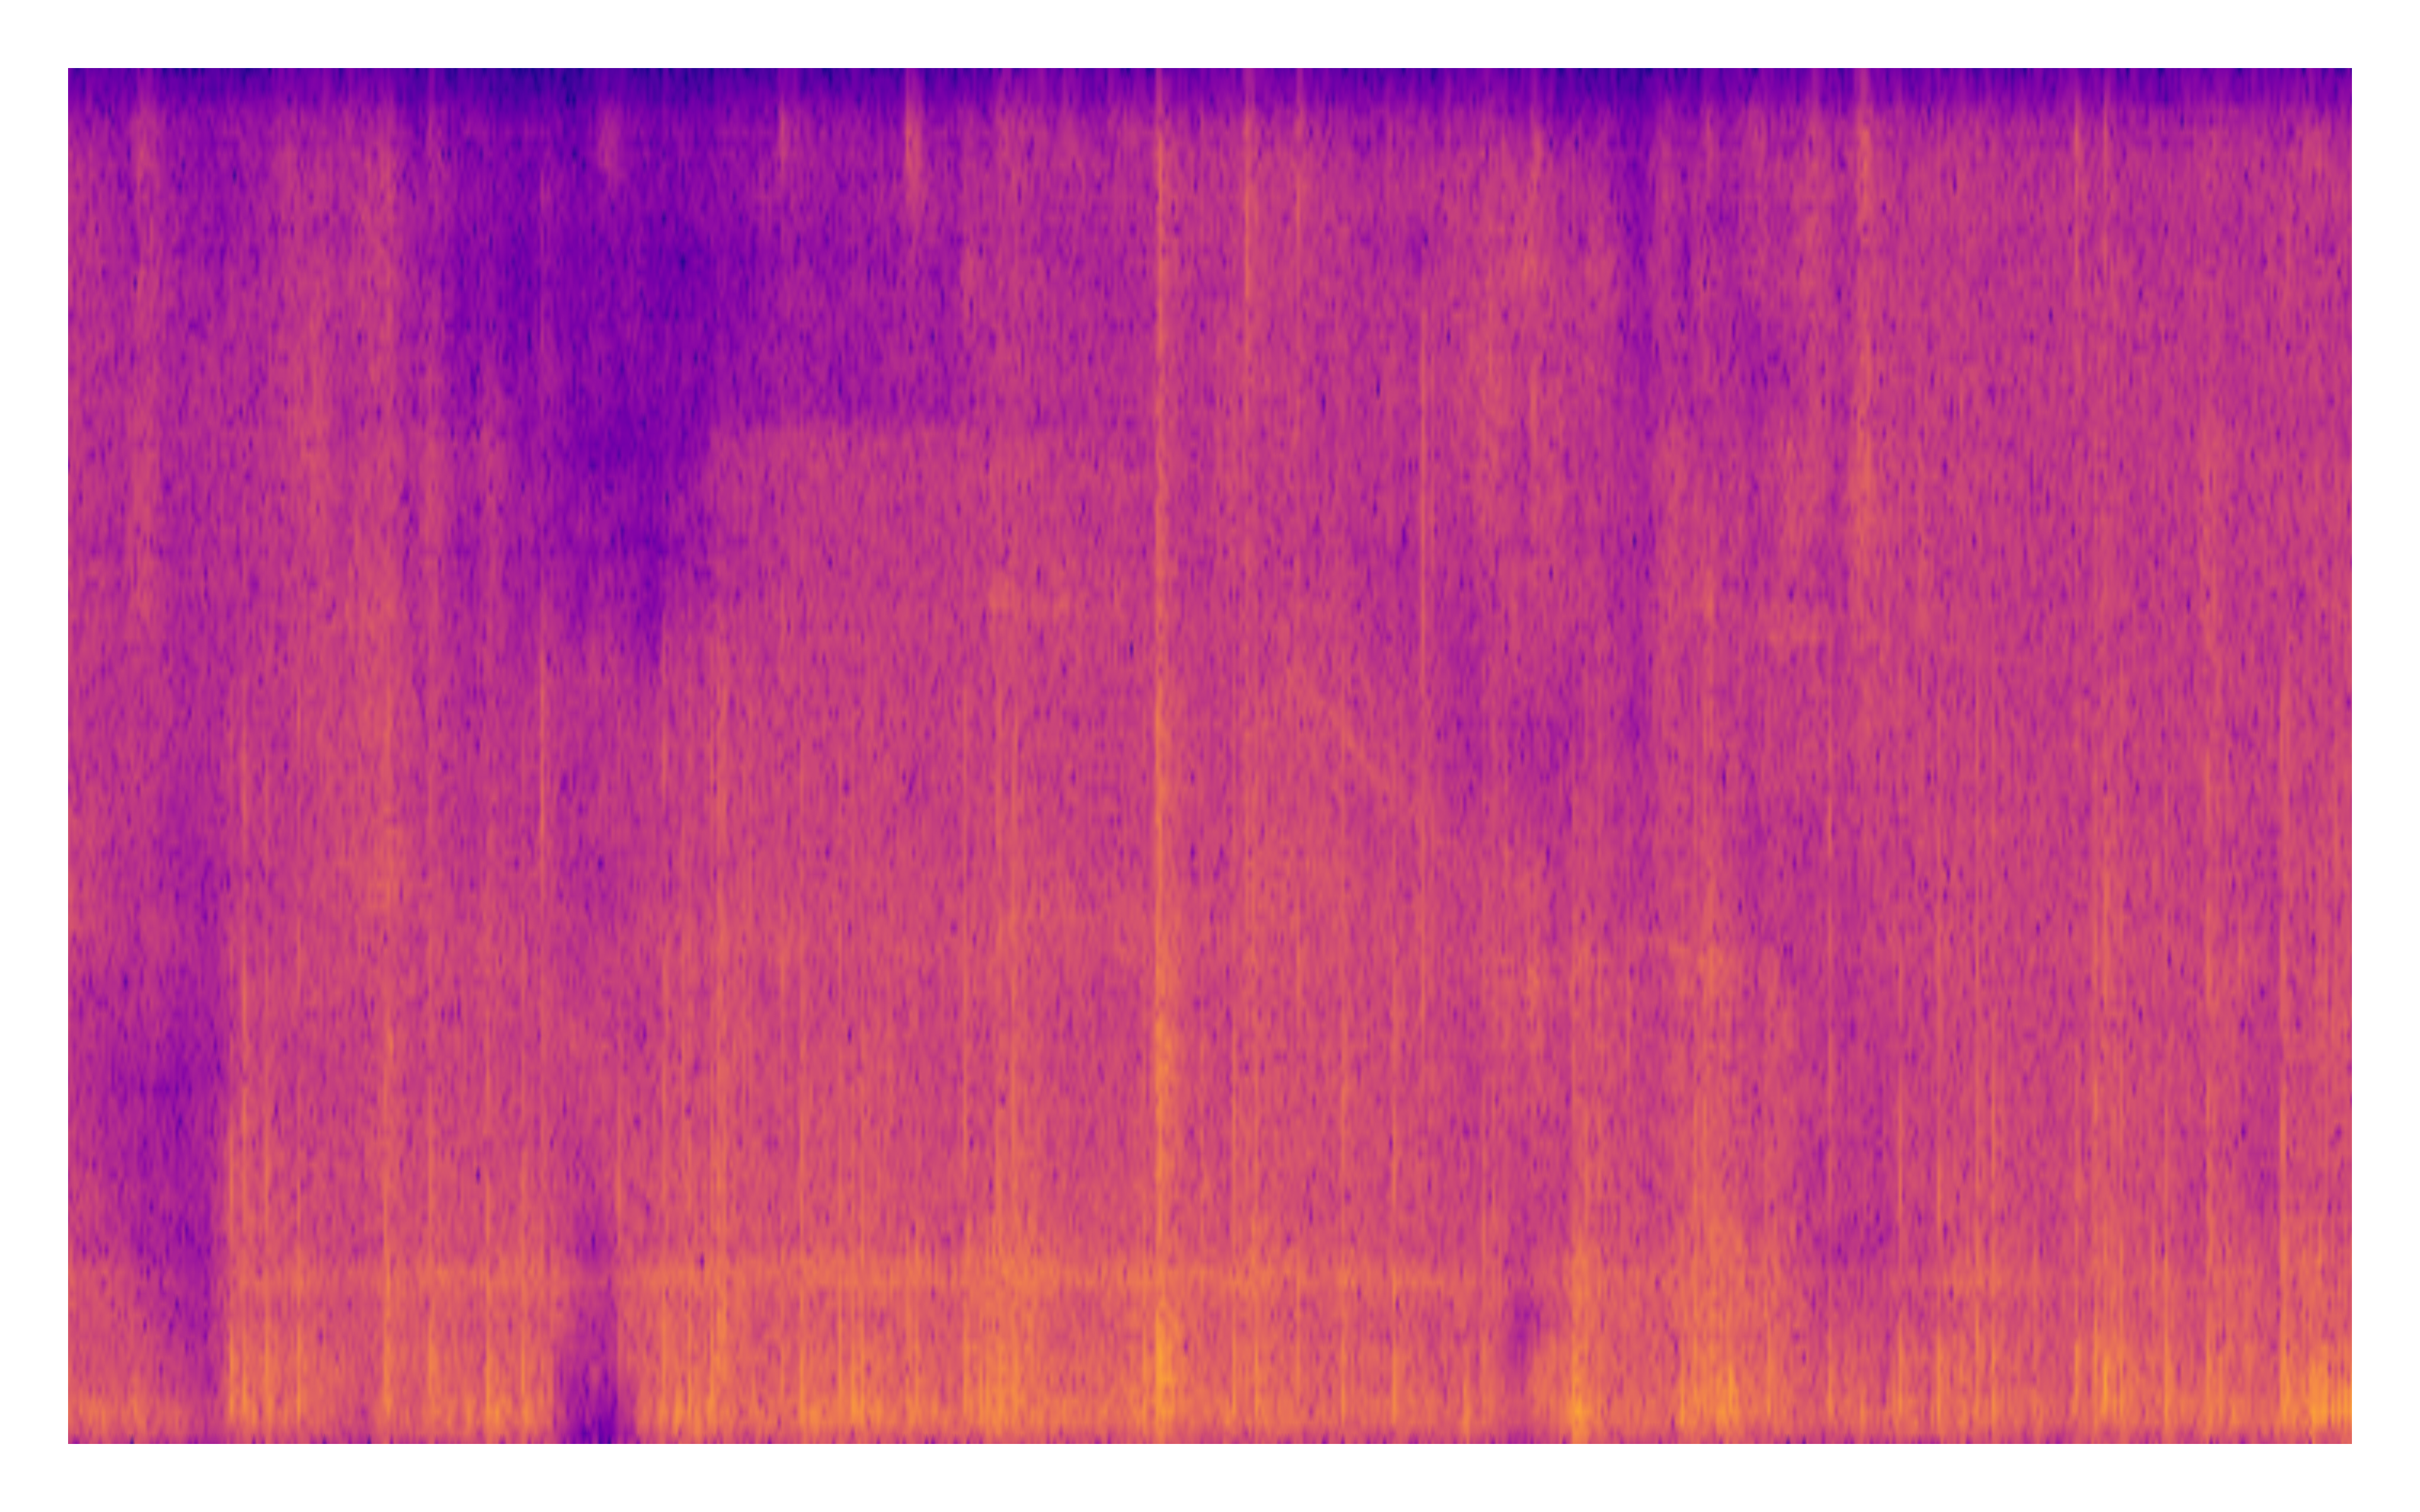
\includegraphics[width=\textwidth]{plots/onepeace_best_delta_similarity/onepeace sep_spectrogram.png}
    \end{subfigure}
    \begin{subfigure}[b]{0.185\textwidth}
        \centering
        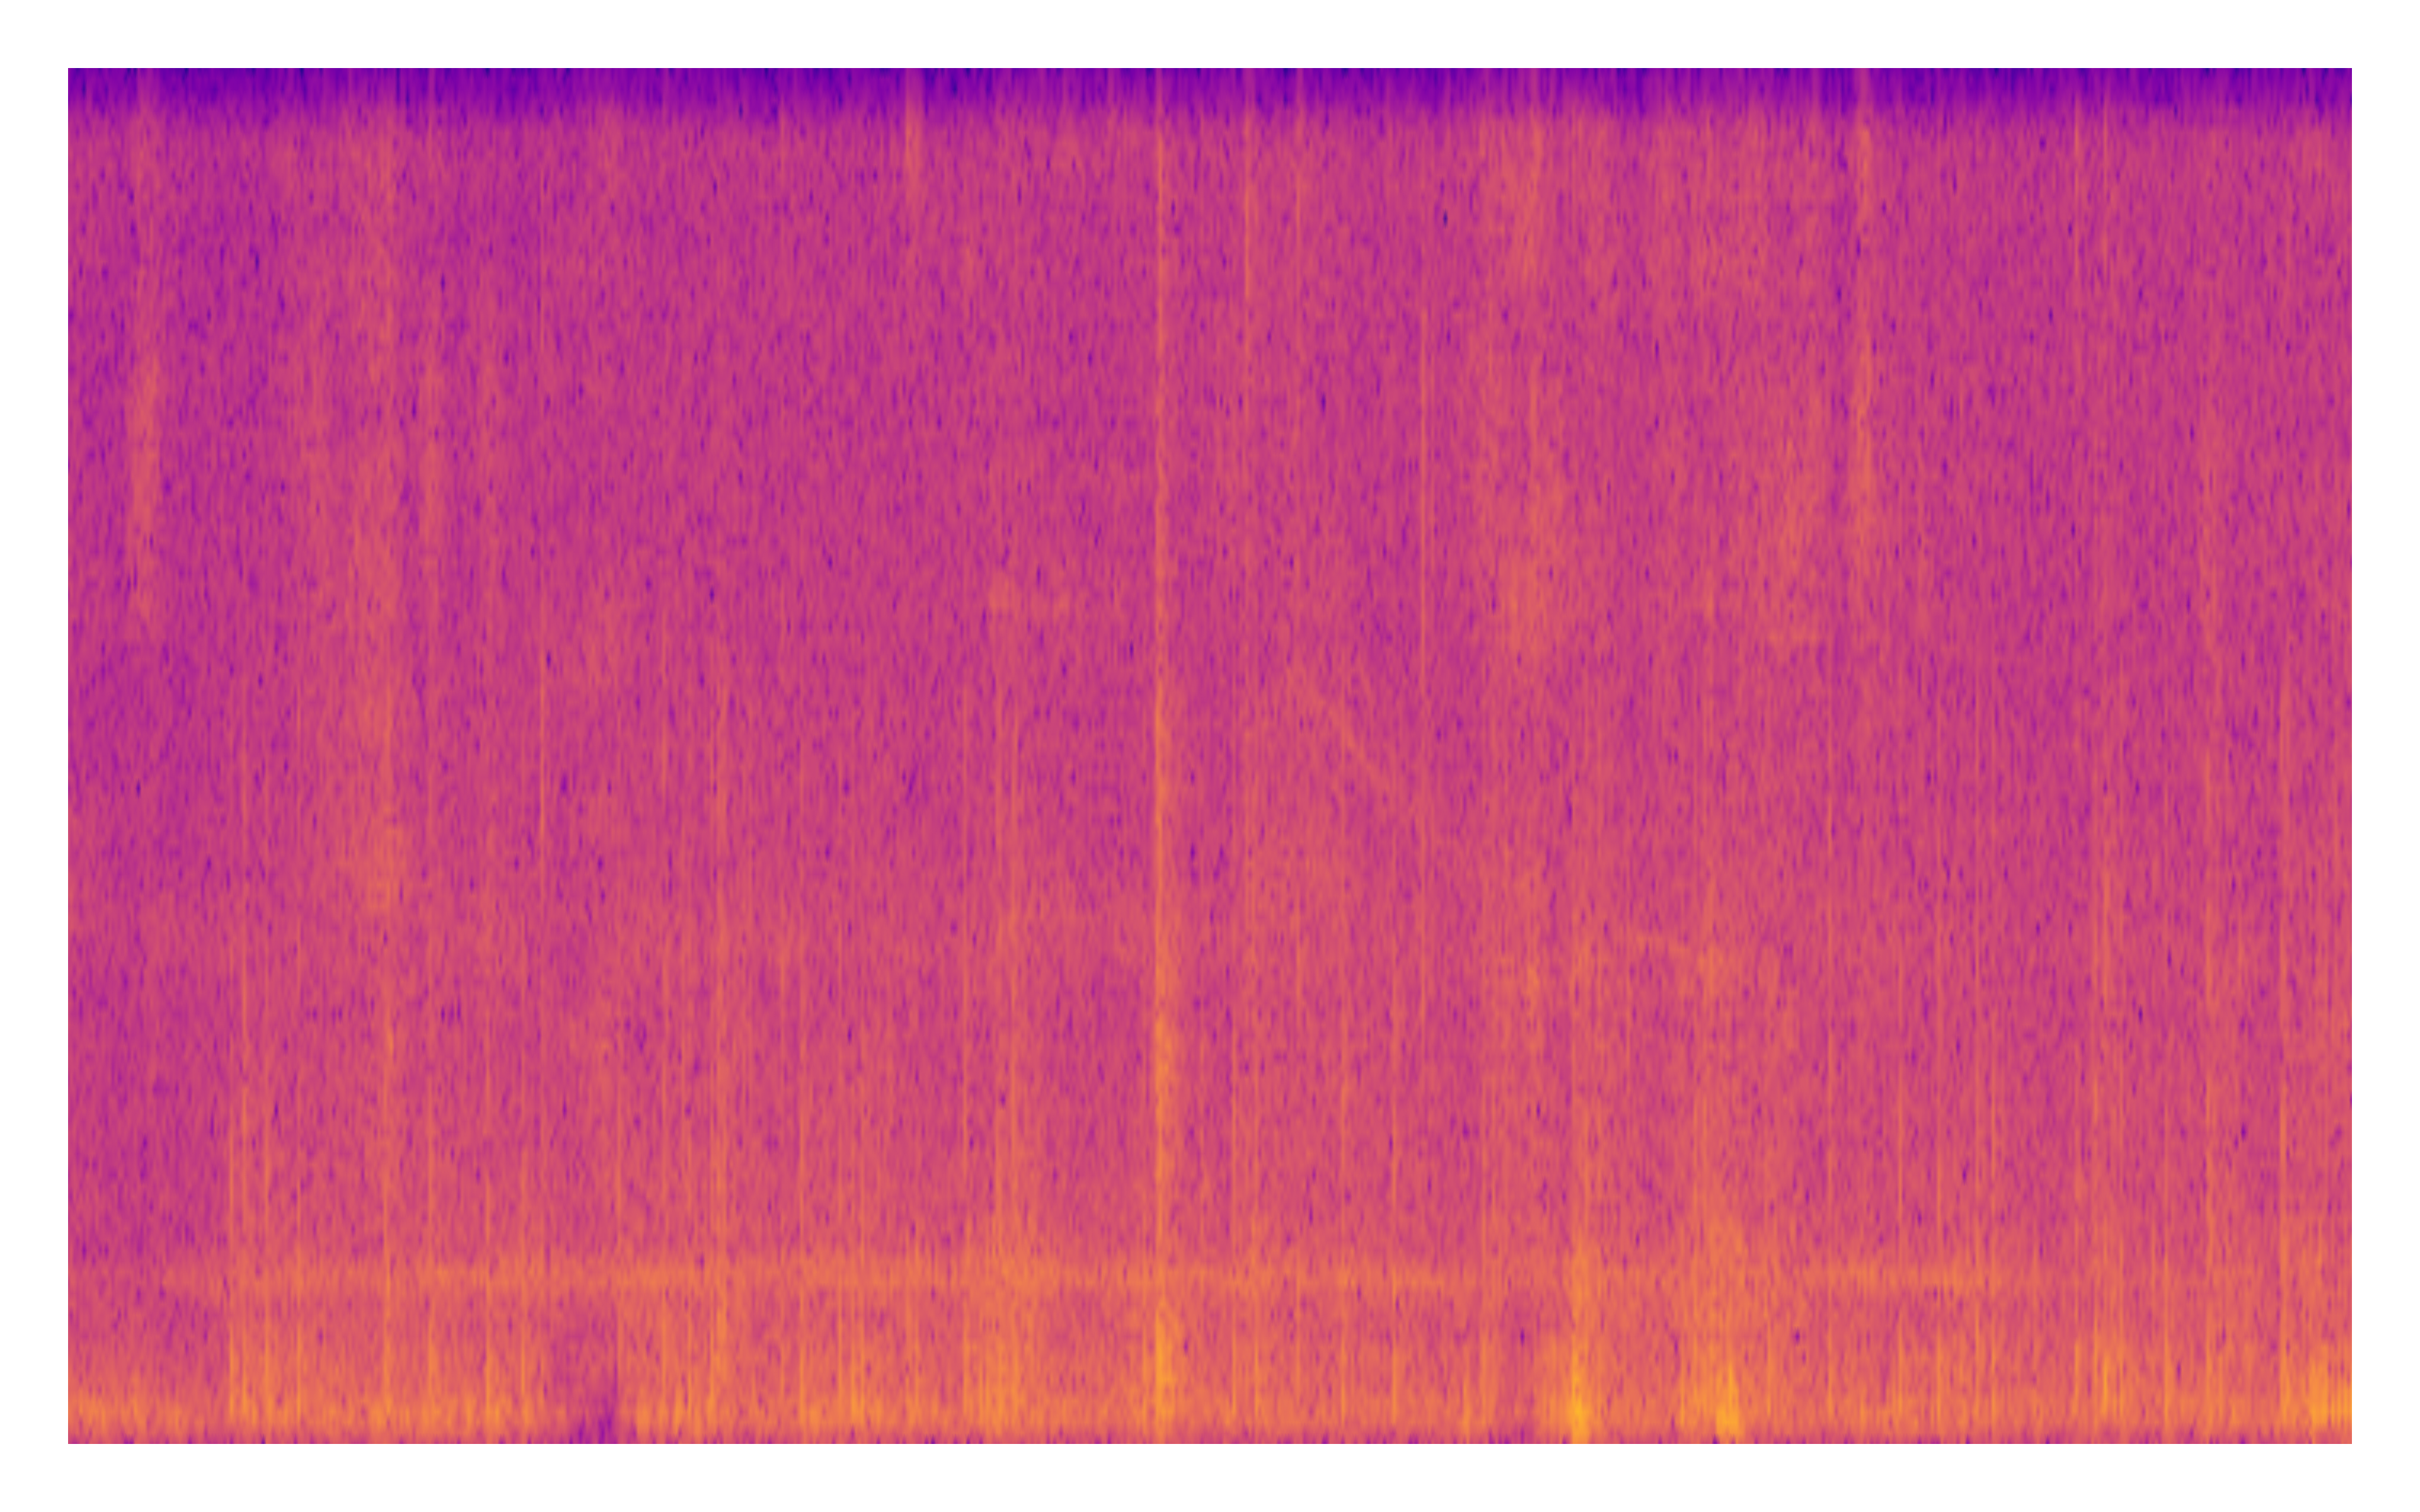
\includegraphics[width=\textwidth]{plots/onepeace_best_delta_similarity/clap sep_spectrogram.png}
    \end{subfigure}
    \begin{subfigure}[b]{0.185\textwidth}
        \centering
        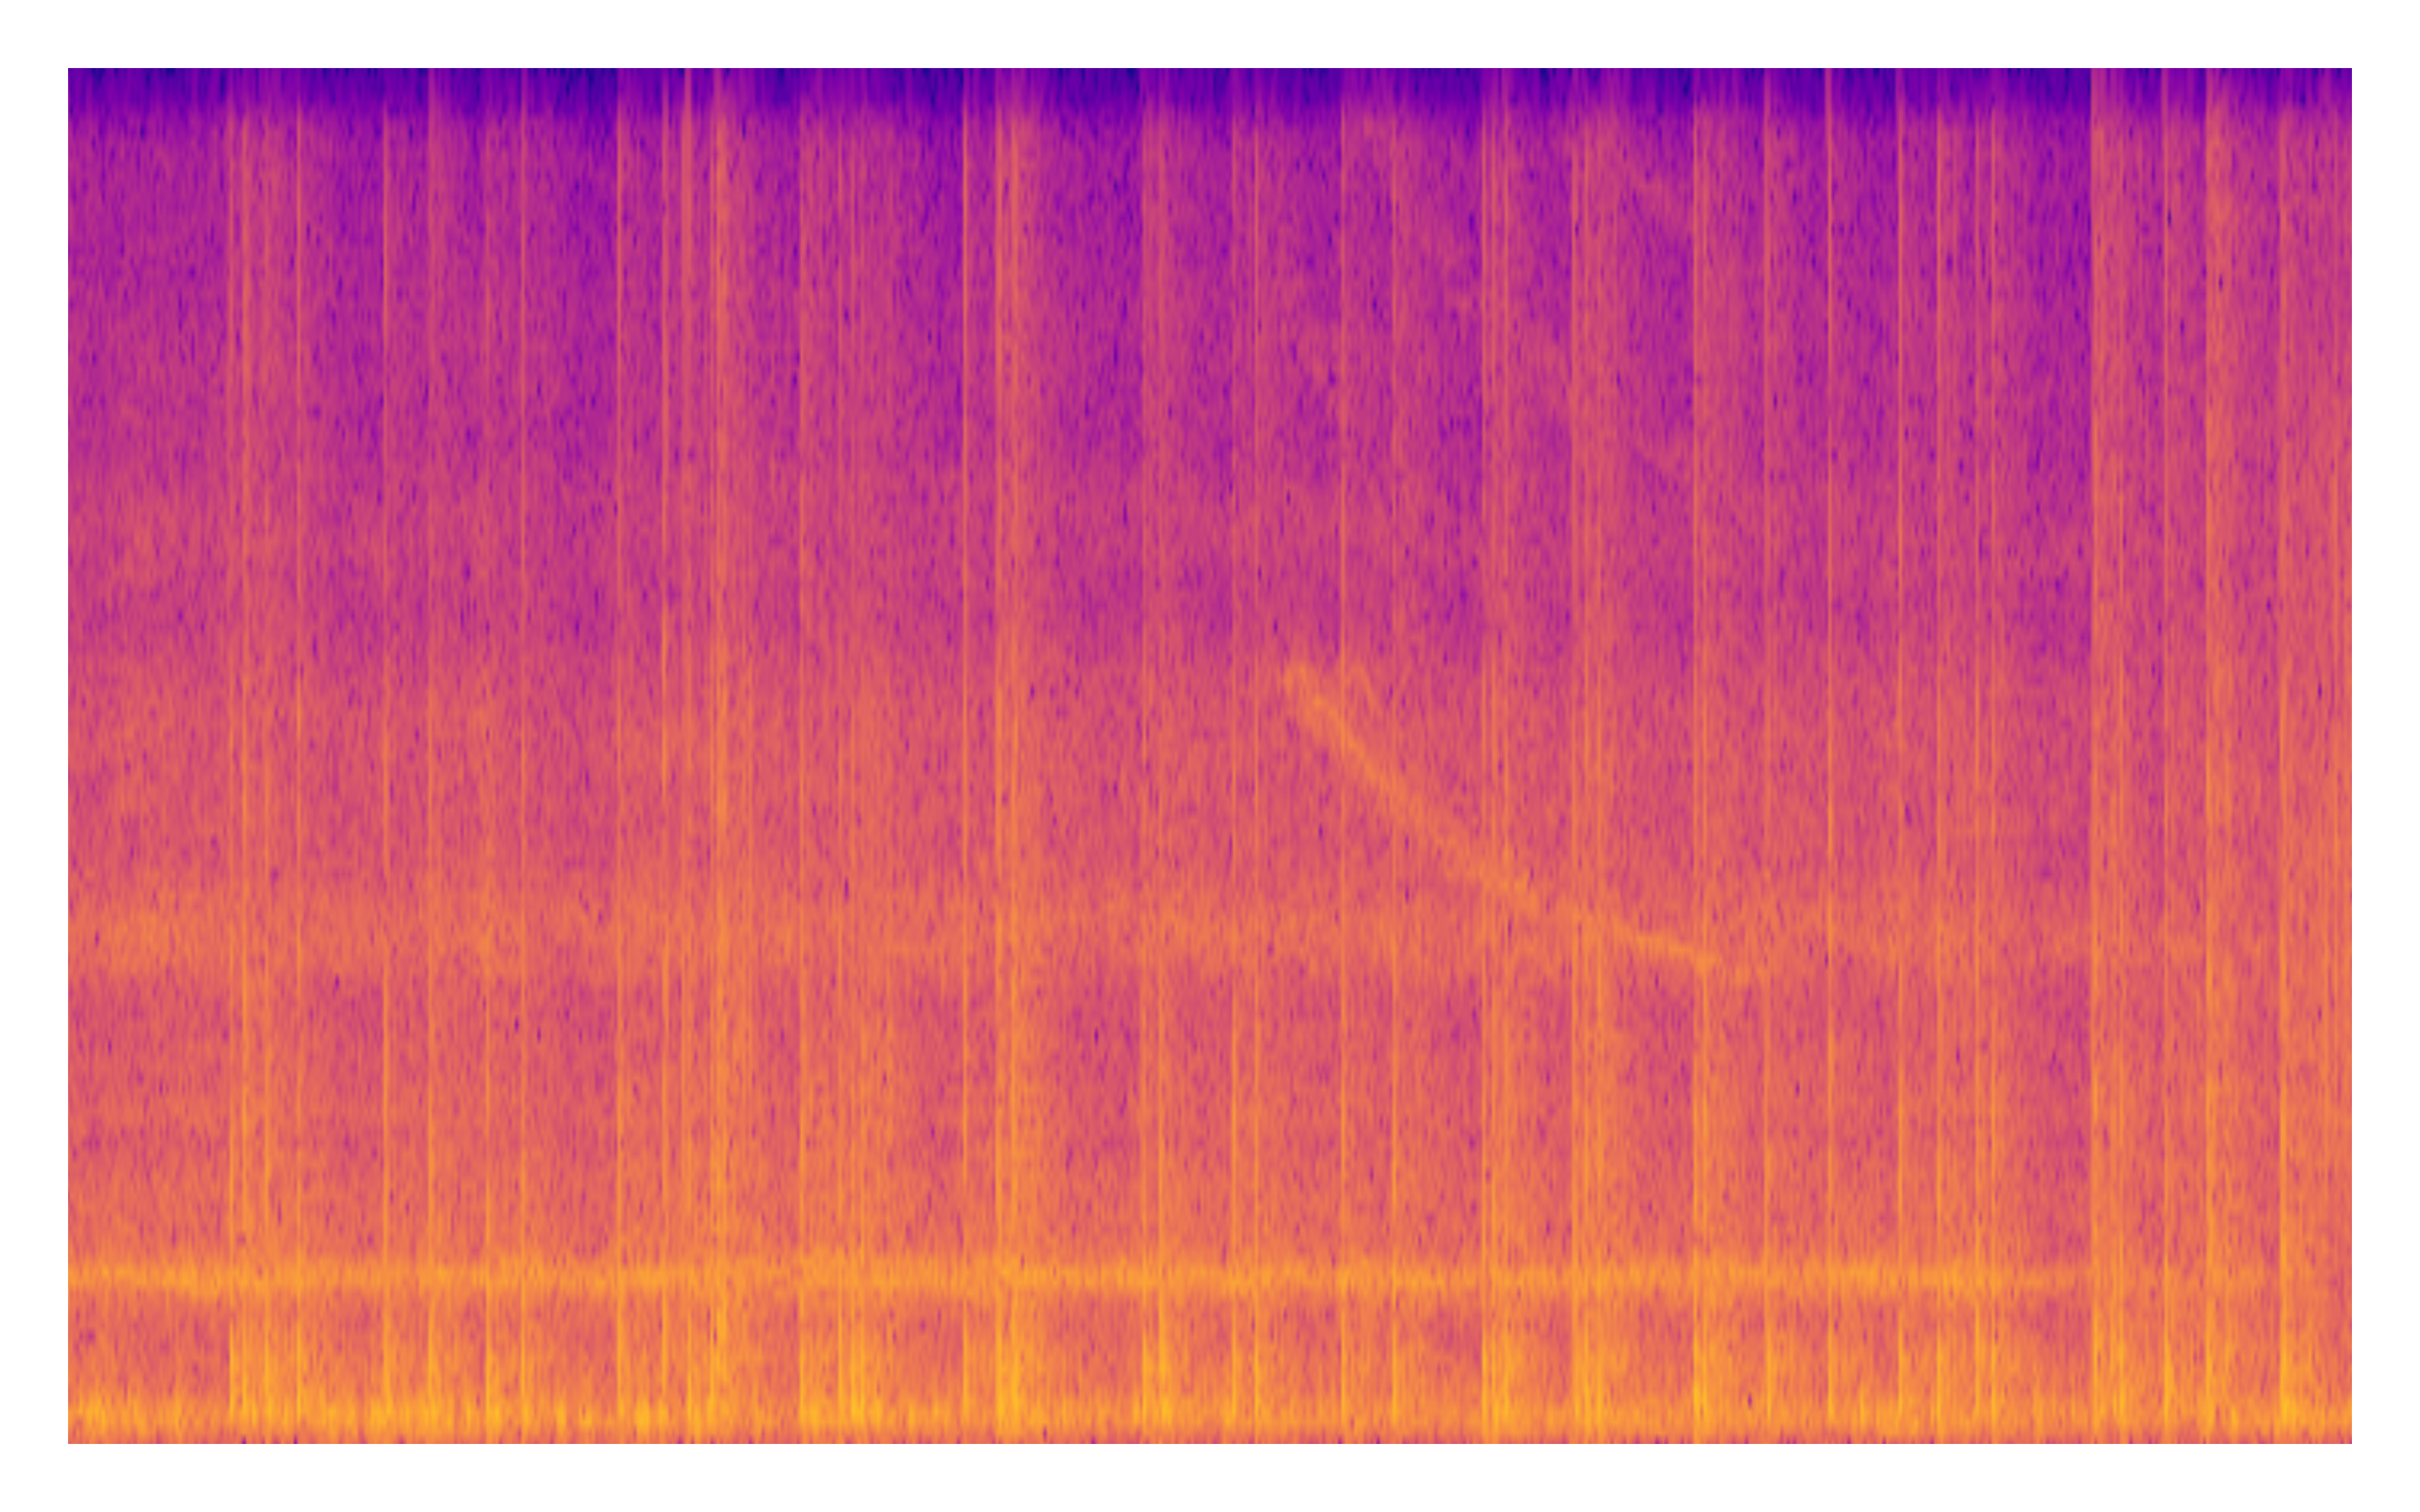
\includegraphics[width=\textwidth]{plots/onepeace_best_delta_similarity/onepeace target_spectrogram.png}
    \end{subfigure}

    % Row: high clap sdr, low onepeace sdr woosh_sound
    \begin{subfigure}[b]{0.185\textwidth}
        \centering
        \scriptsize\textbf{"A whooshing sound is moving rapidly"}
        \vspace{5.0mm}
        \caption*{Language Query}
    \end{subfigure}
    \begin{subfigure}[b]{0.185\textwidth}
        \centering
        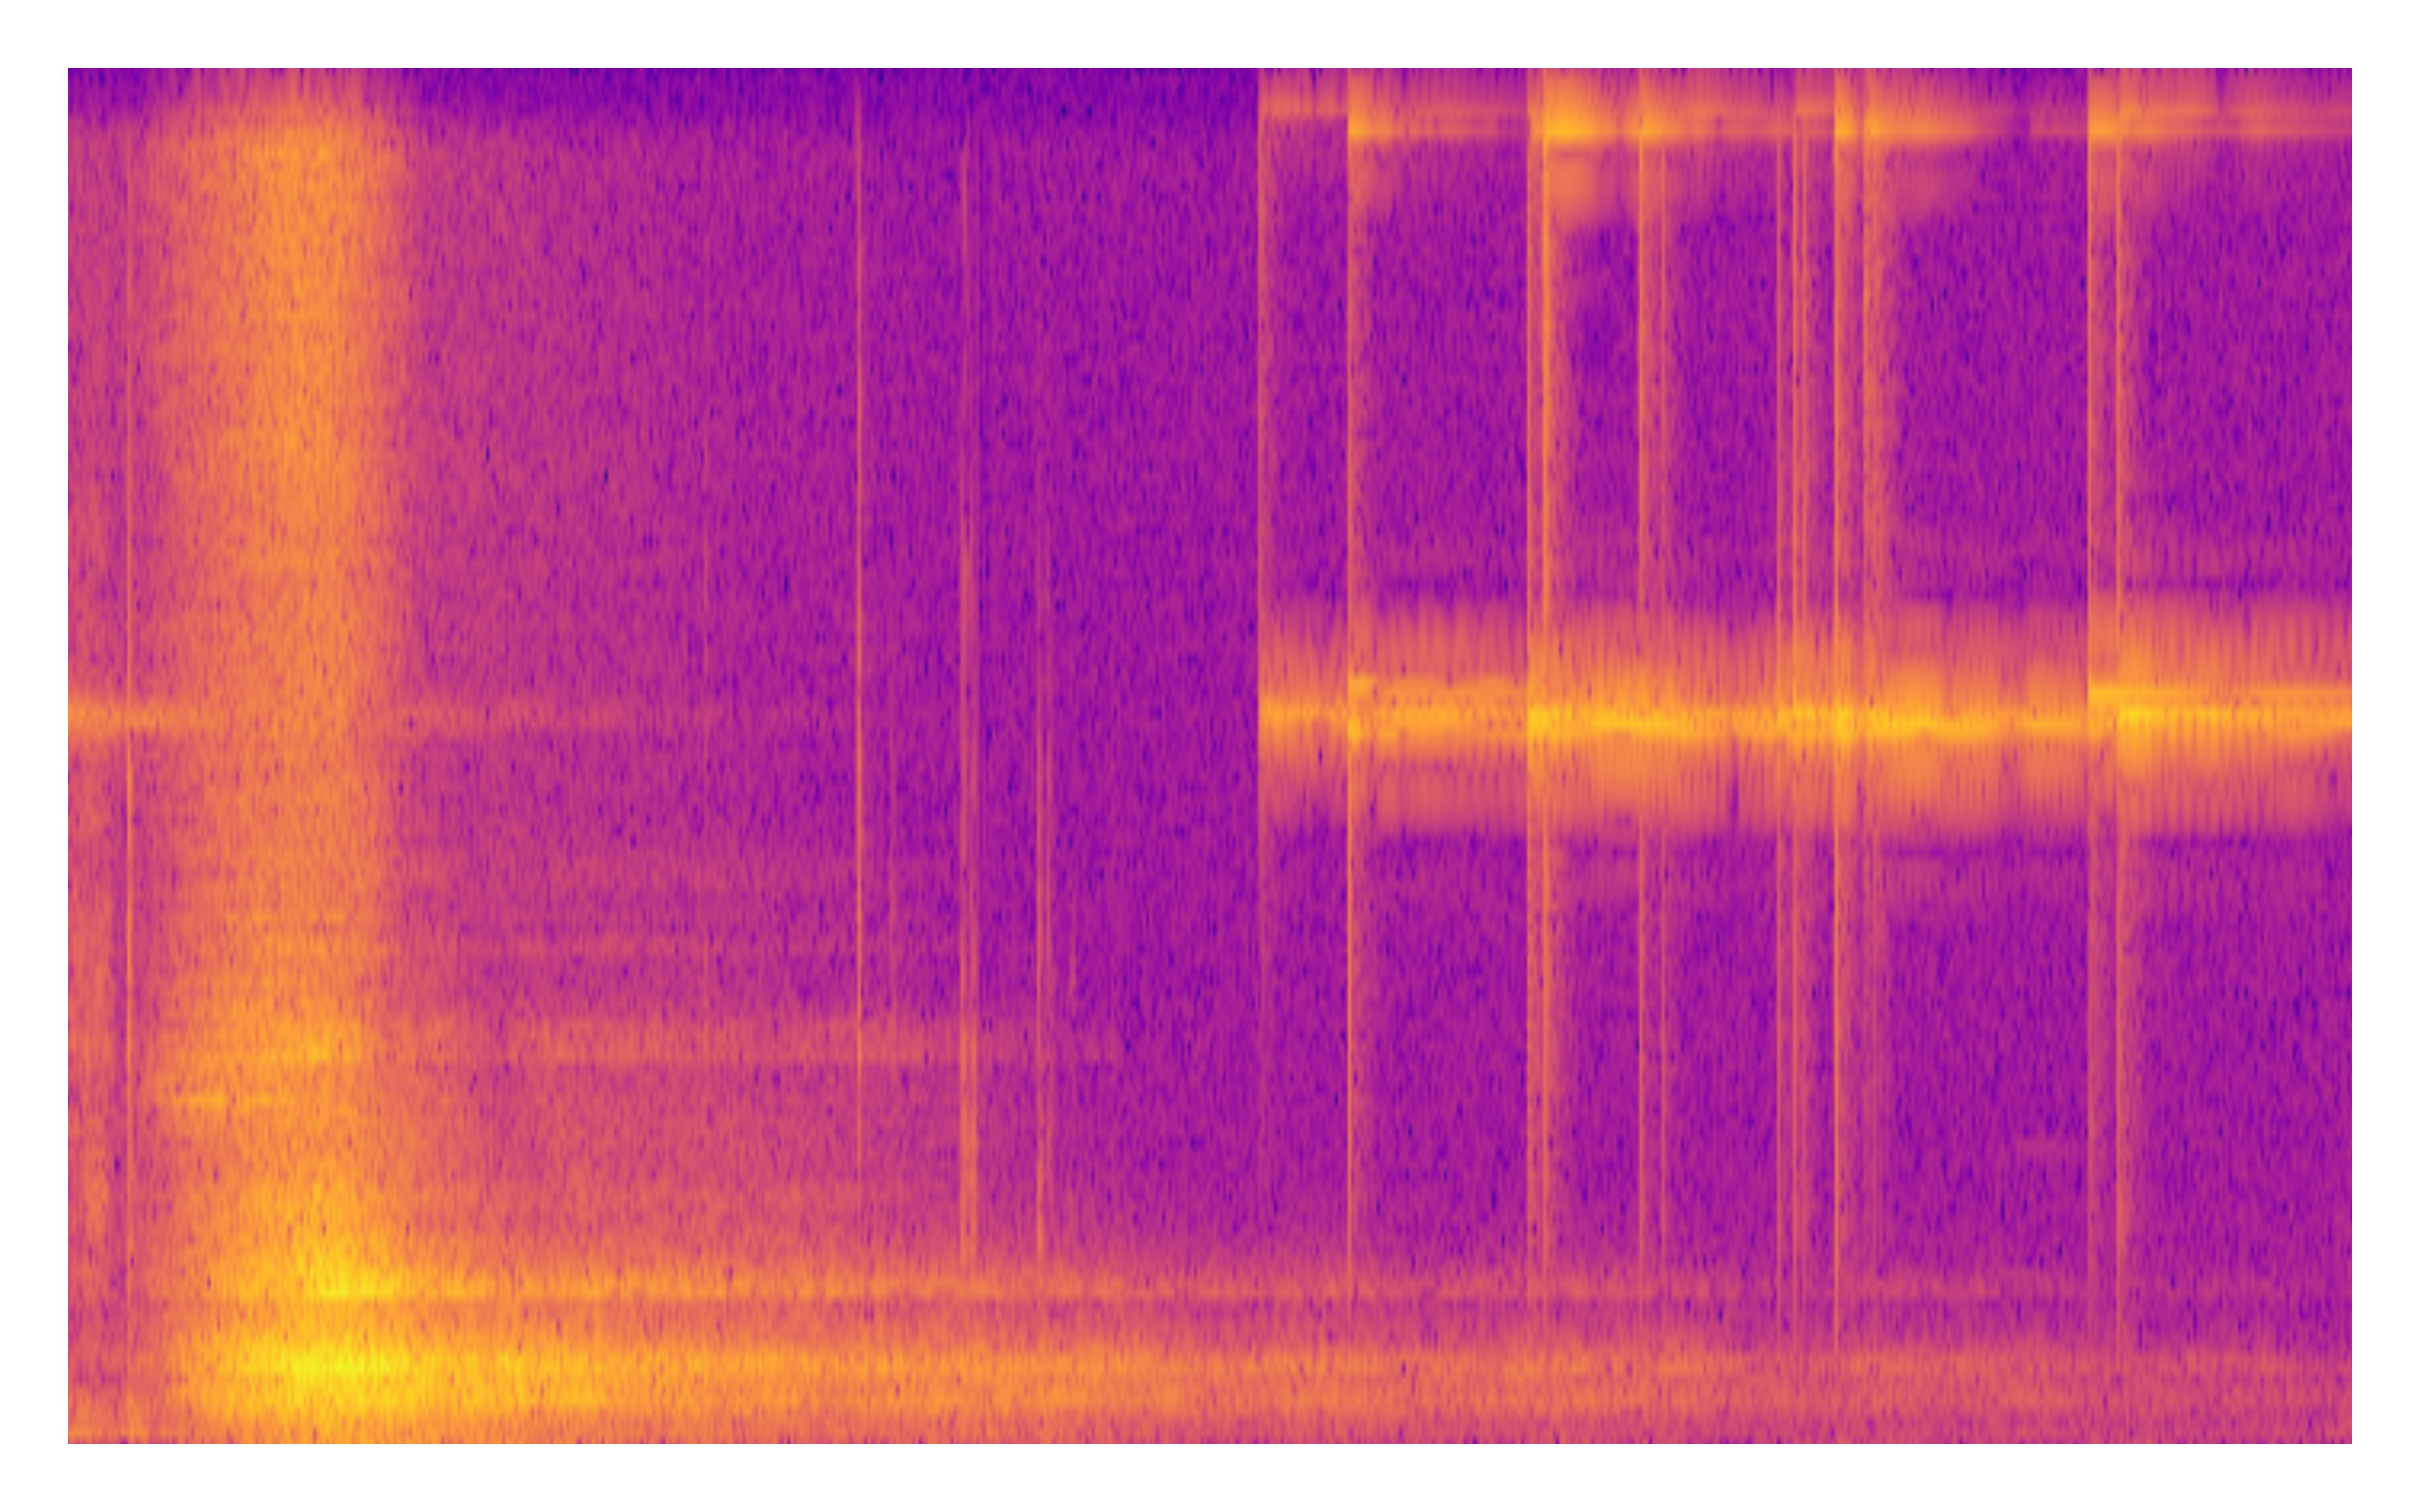
\includegraphics[width=\textwidth]{plots/whooshing_sound/clap mixture_spectrogram.png}
        \centering
        \caption*{Mixture}
    \end{subfigure}
    \begin{subfigure}[b]{0.185\textwidth}
        \centering
        \includegraphics[width=\textwidth]{plots/whooshing_sound/onepeace sep_spectrogram.png}
        \caption*{ONE-PEACE}
    \end{subfigure}
    \begin{subfigure}[b]{0.185\textwidth}
        \centering
        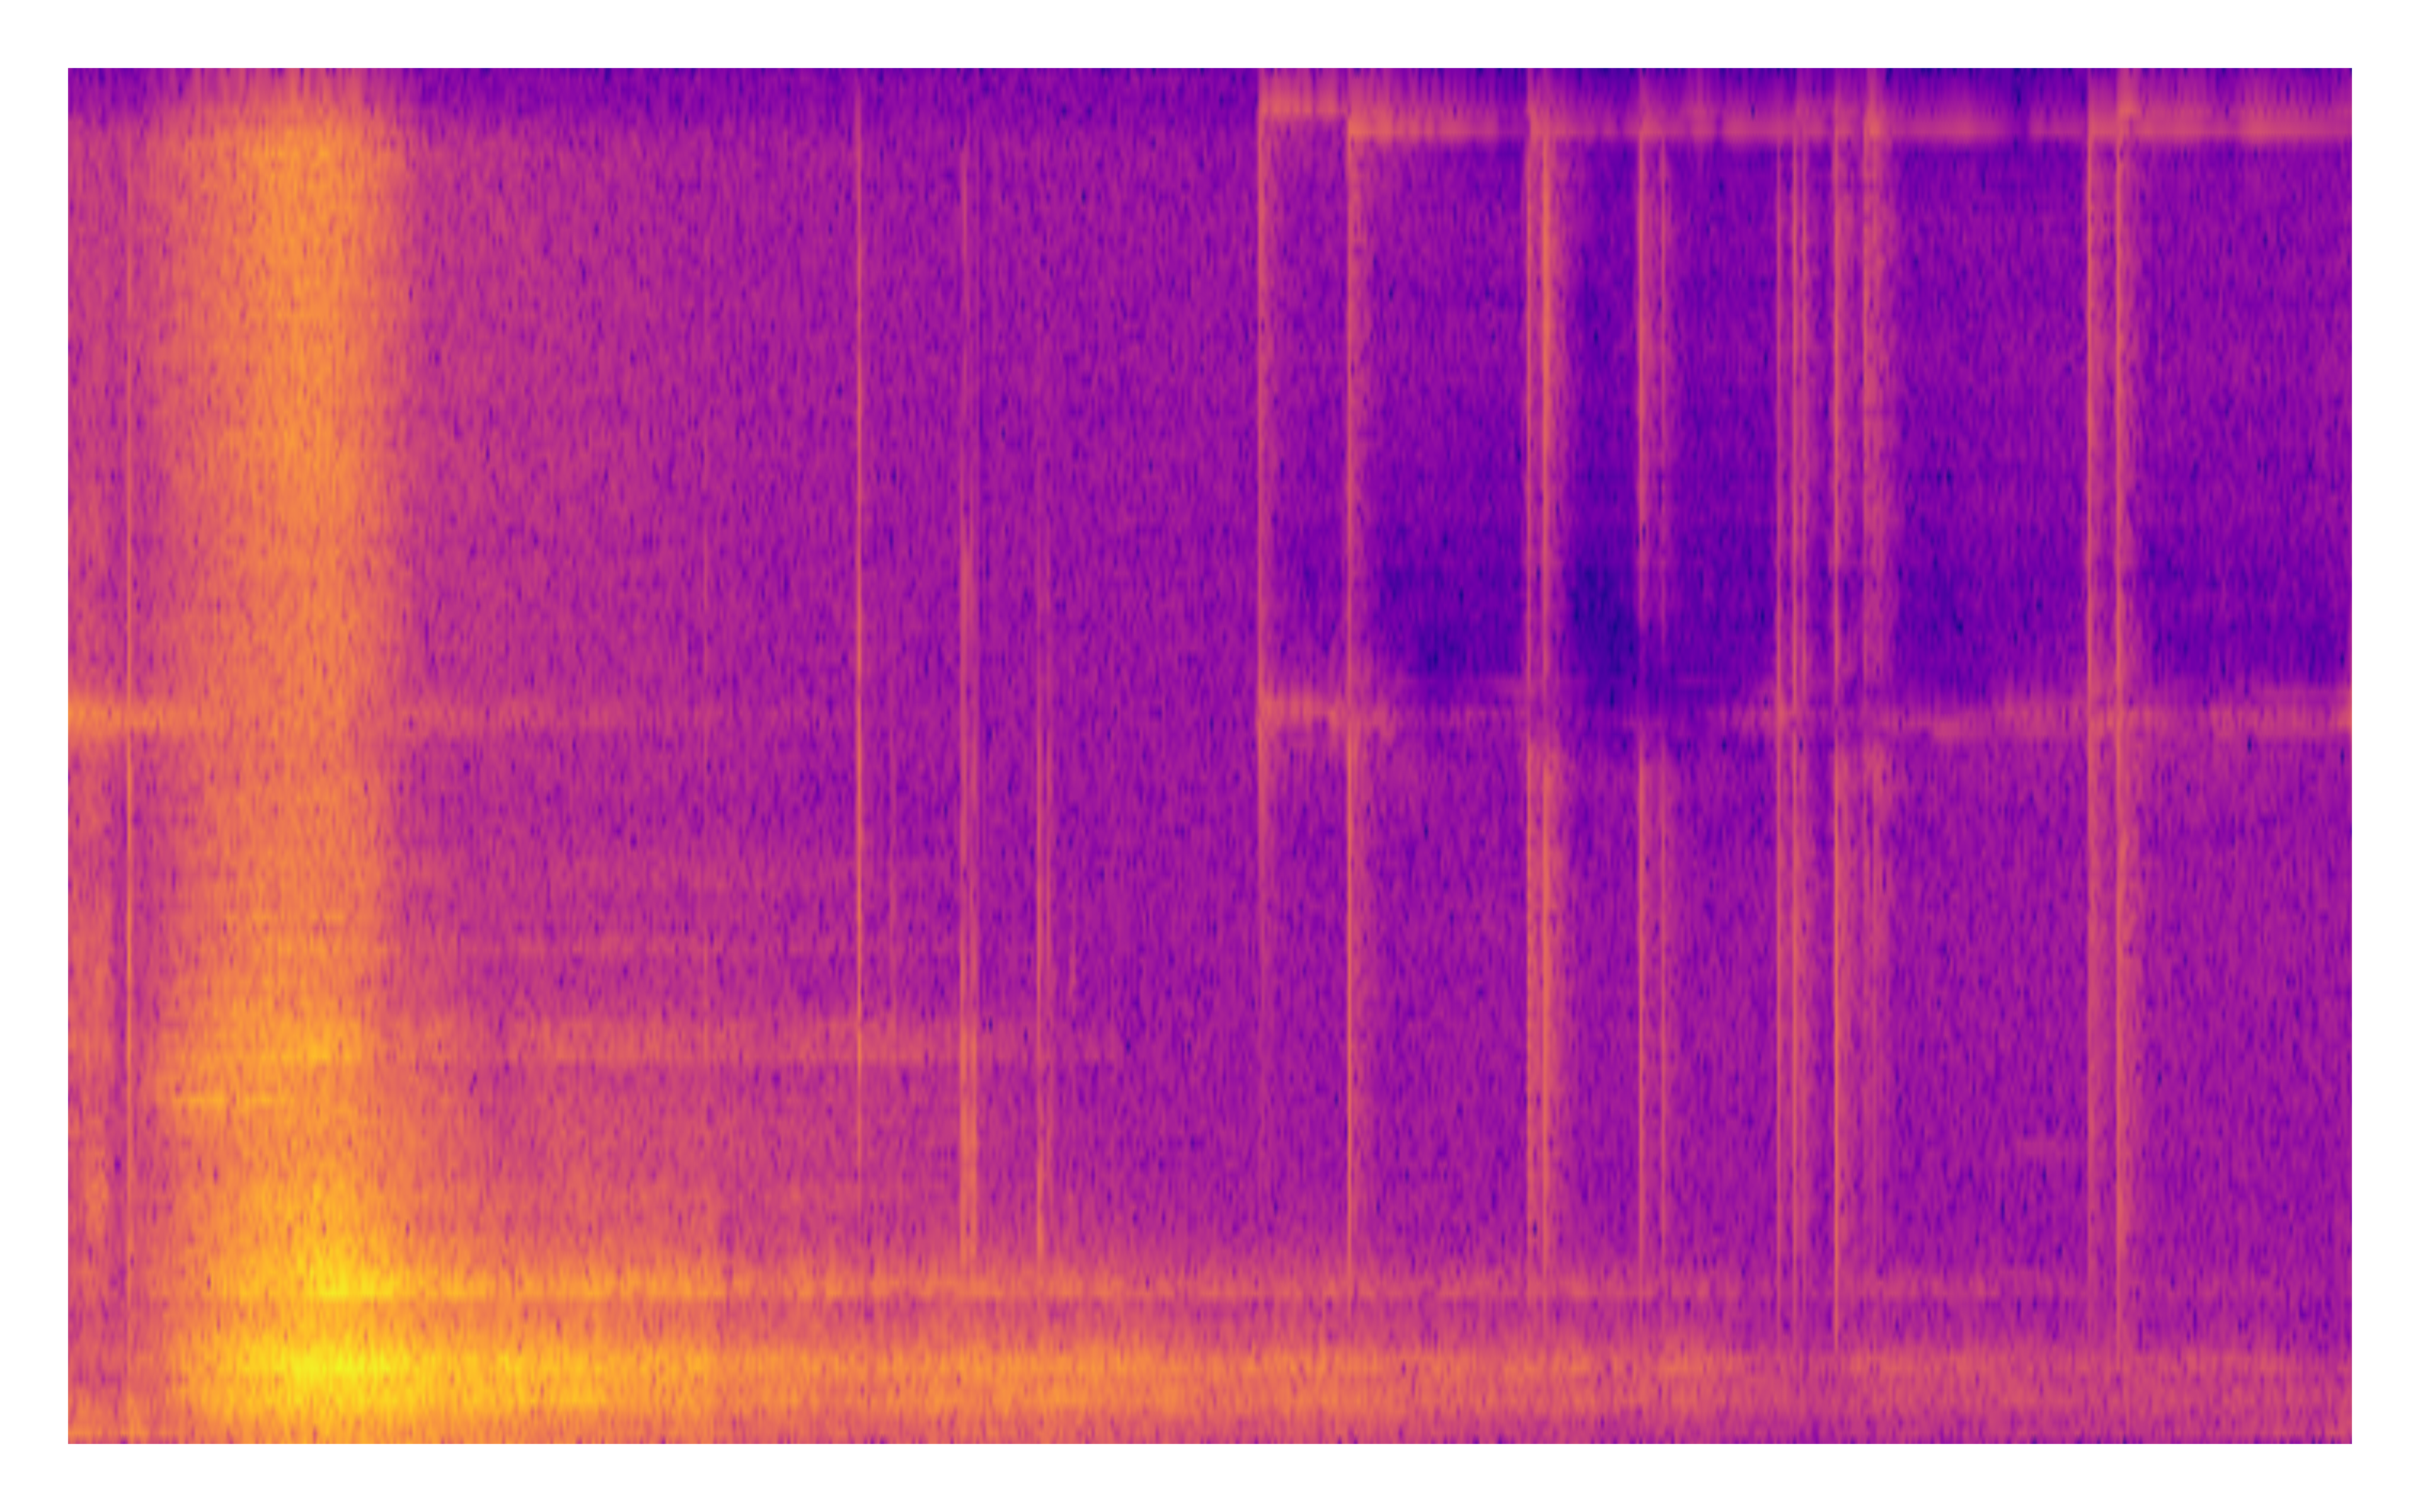
\includegraphics[width=\textwidth]{plots/whooshing_sound/clap sep_spectrogram.png}
        \caption*{CLAP}
    \end{subfigure}
    \begin{subfigure}[b]{0.185\textwidth}
        \centering
        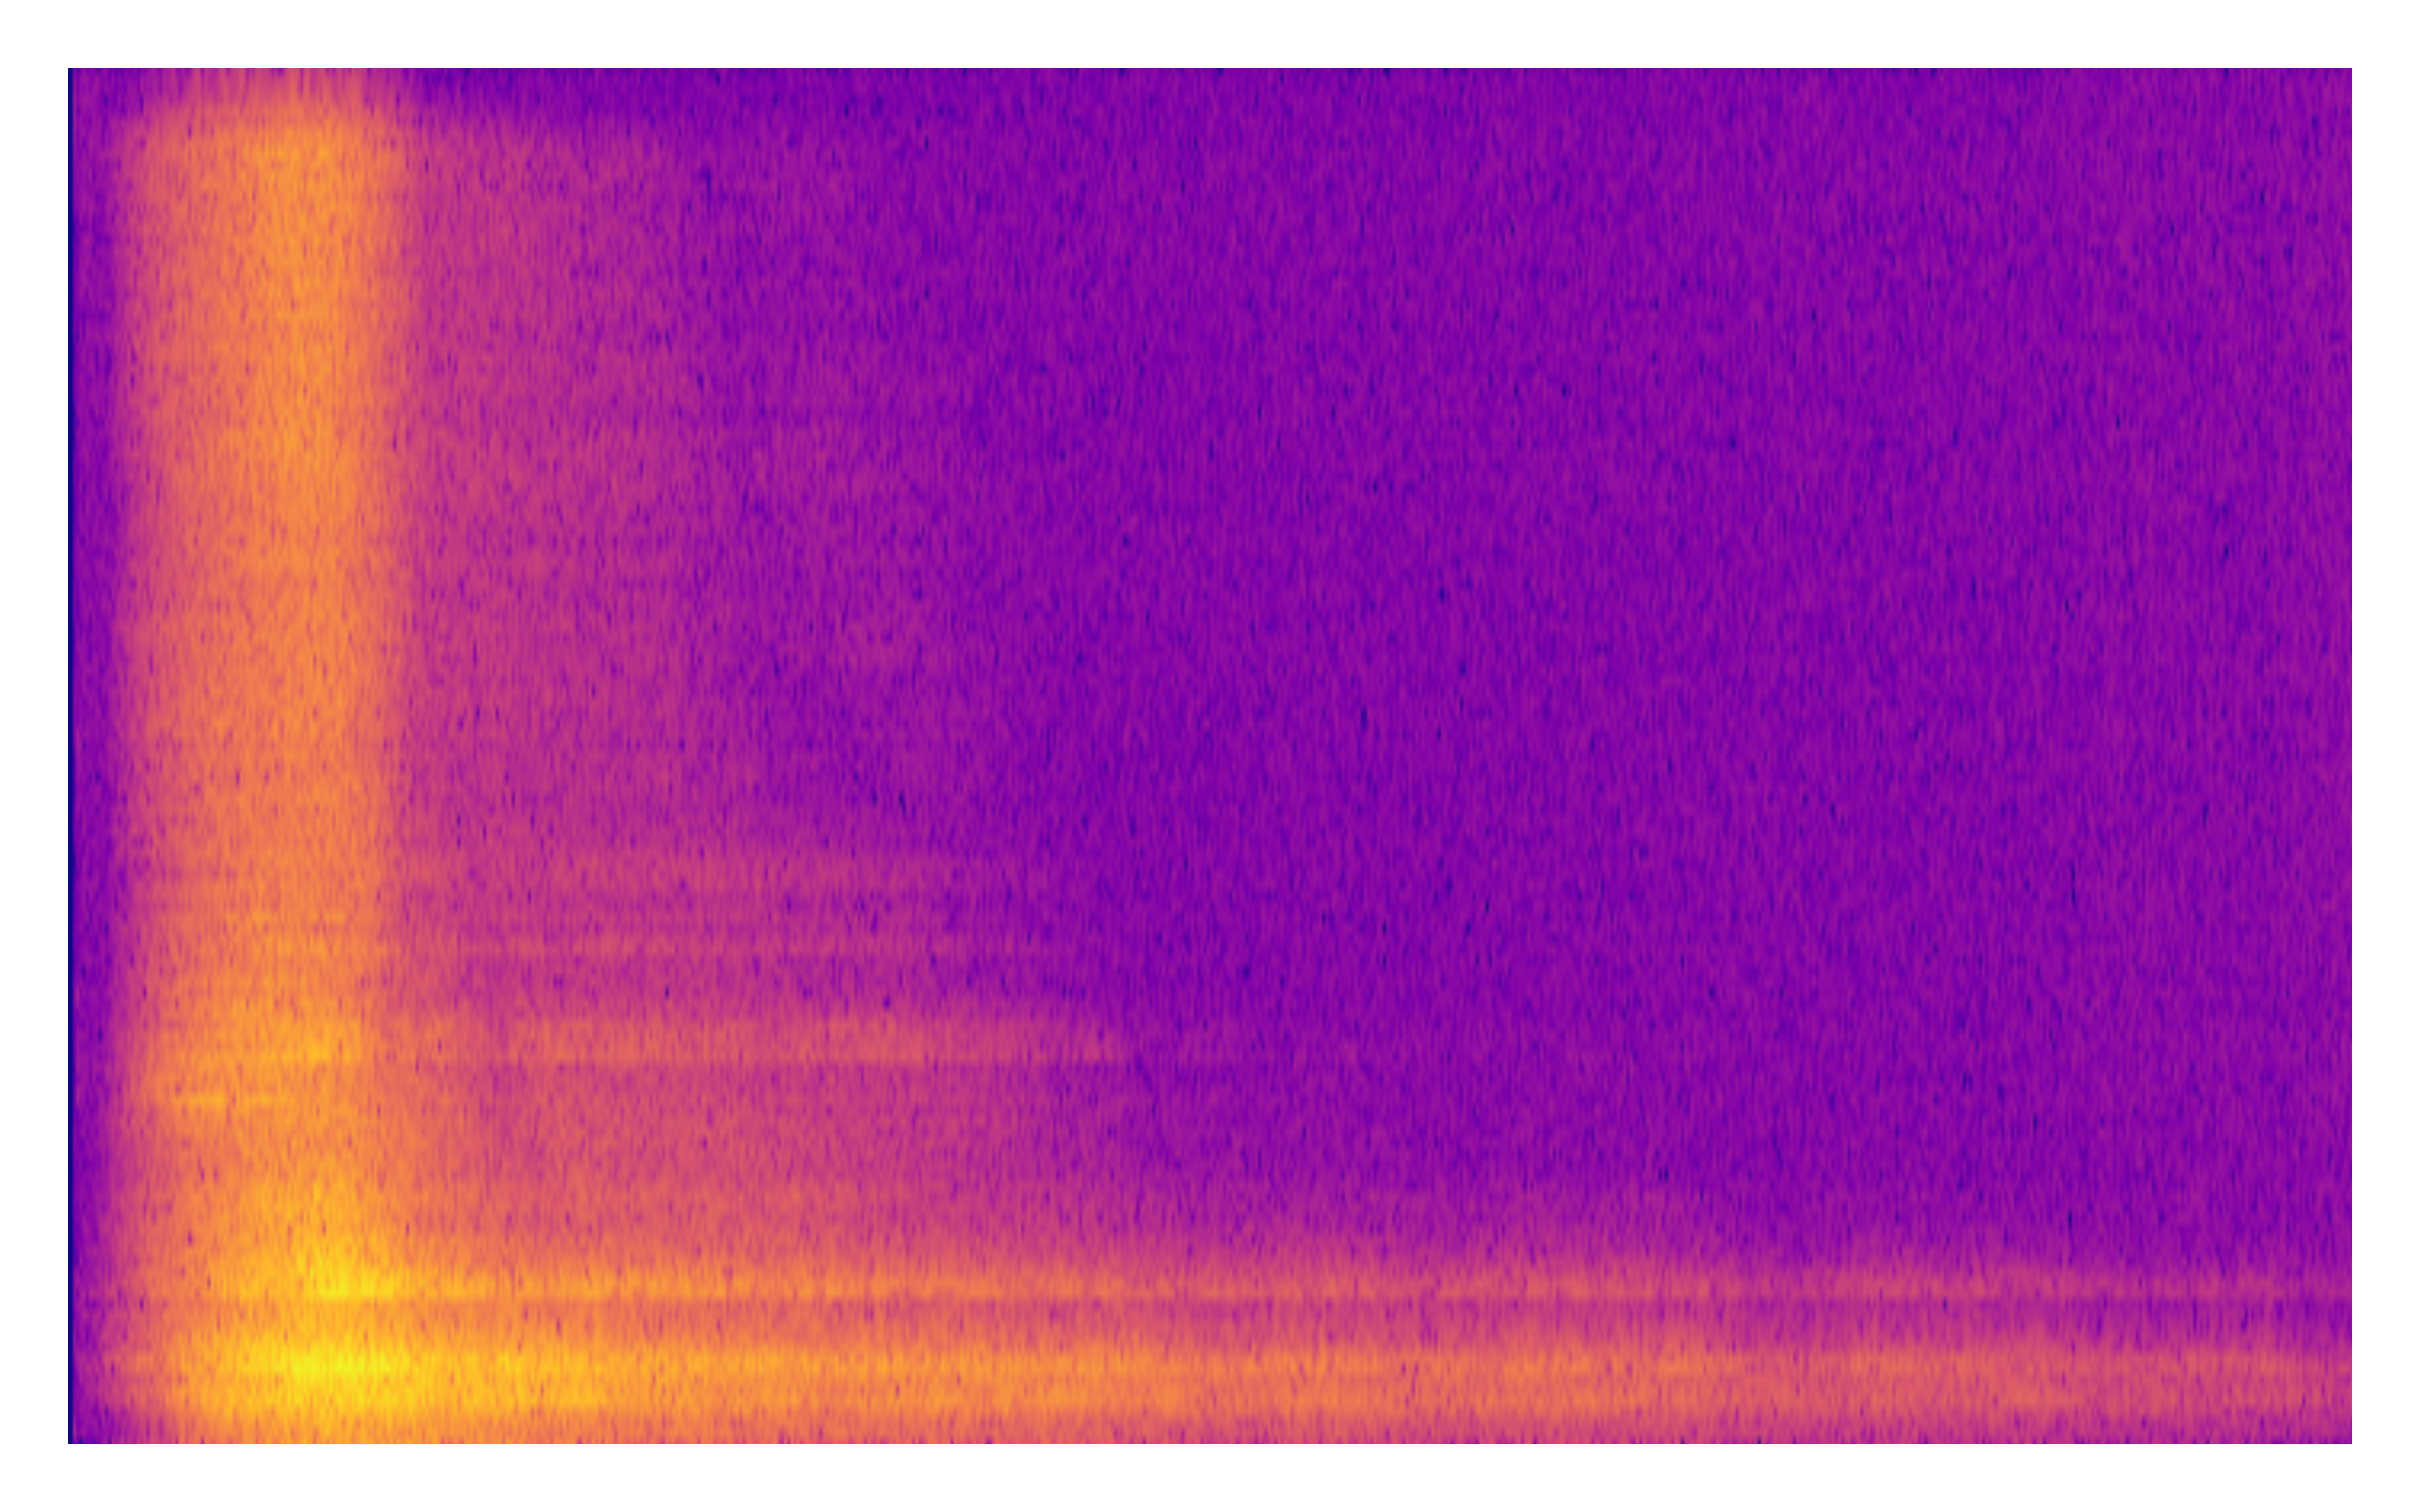
\includegraphics[width=\textwidth]{plots/whooshing_sound/clap target_spectrogram.png}
        \caption*{Target}
    \end{subfigure}
    
    % Continue rows similarly for other queries
    % Add caption below
    \caption{Visualized spectrograms for various language queries from the DCASE 2024 T9 Validation Set. The x-axis represents time, the y-axis represents the frequency of the signal, and the hue represents the power (decibels), where brighter colors have higher power.}
    
    \label{fig:separation_results}

\end{figure*}

\label{fig:val_visuals}

\begin{figure*}[!htbp]

    % Row: input mixture and target
    \begin{subfigure}[b]{0.3\textwidth}
        \centering
        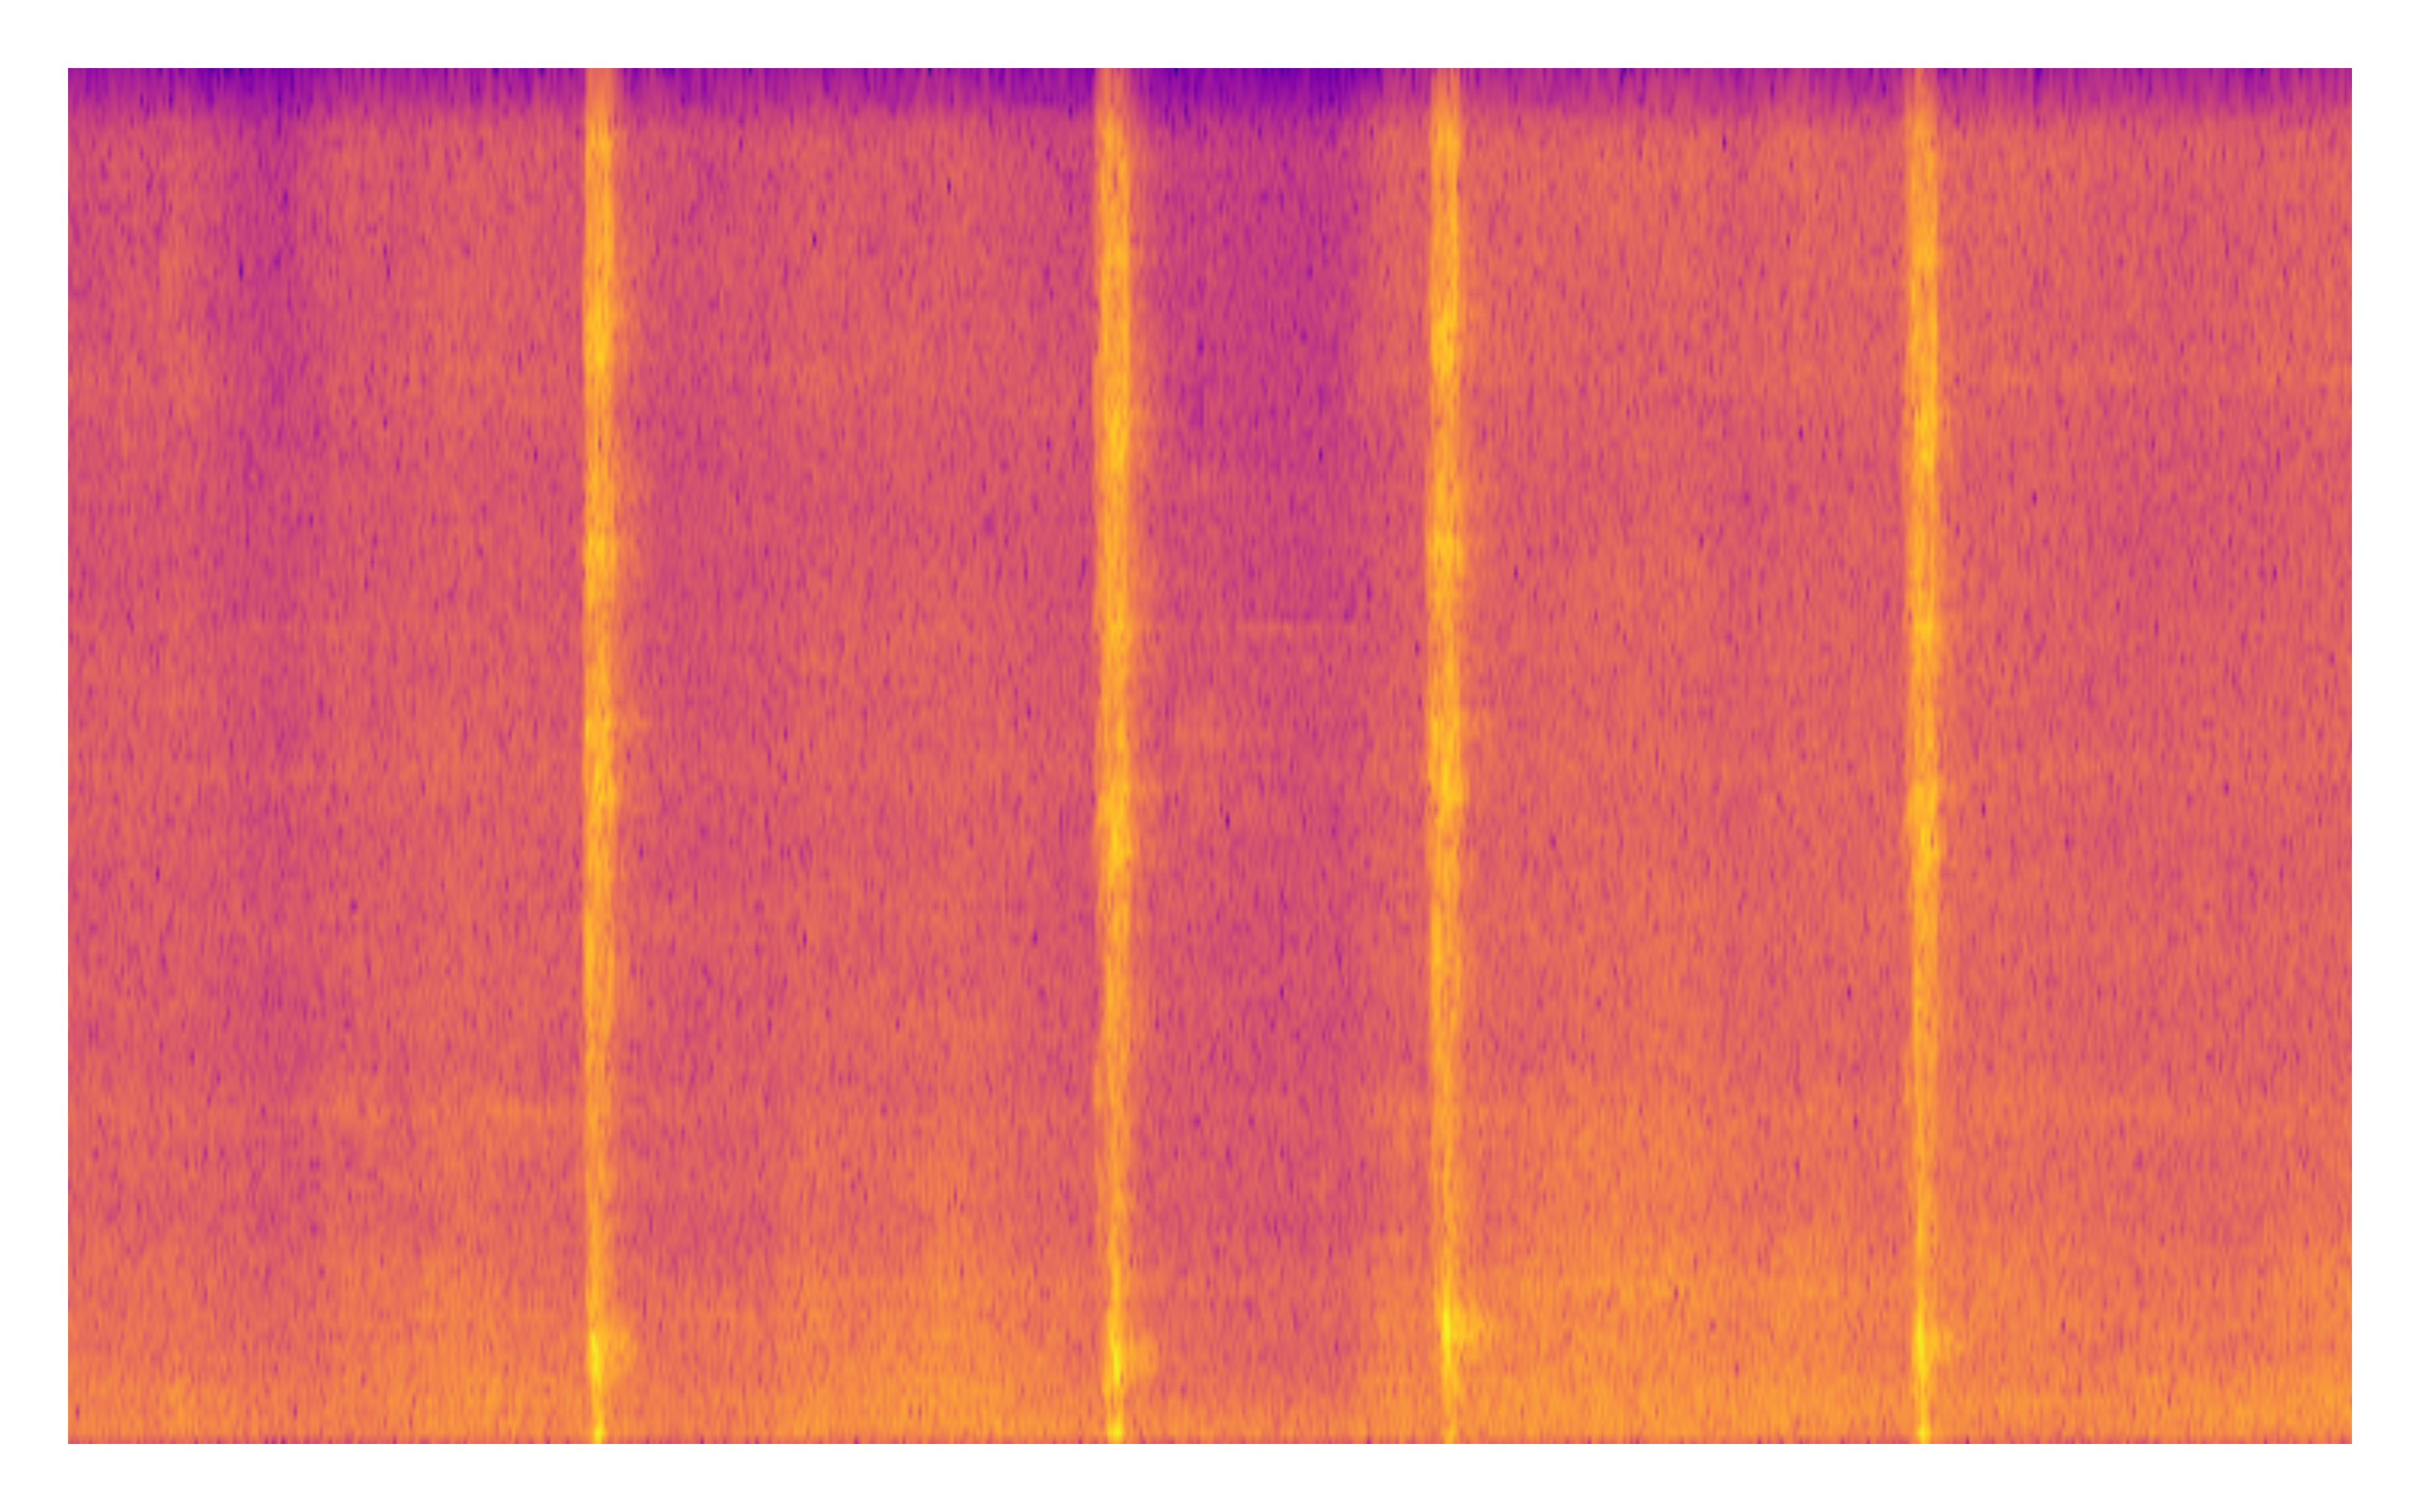
\includegraphics[width=\textwidth]{plots/sword_swoosh/clap mixture_spectrogram.png}
        \caption*{Mixture}
    \end{subfigure}
    \begin{subfigure}[b]{0.3\textwidth}
        \centering
        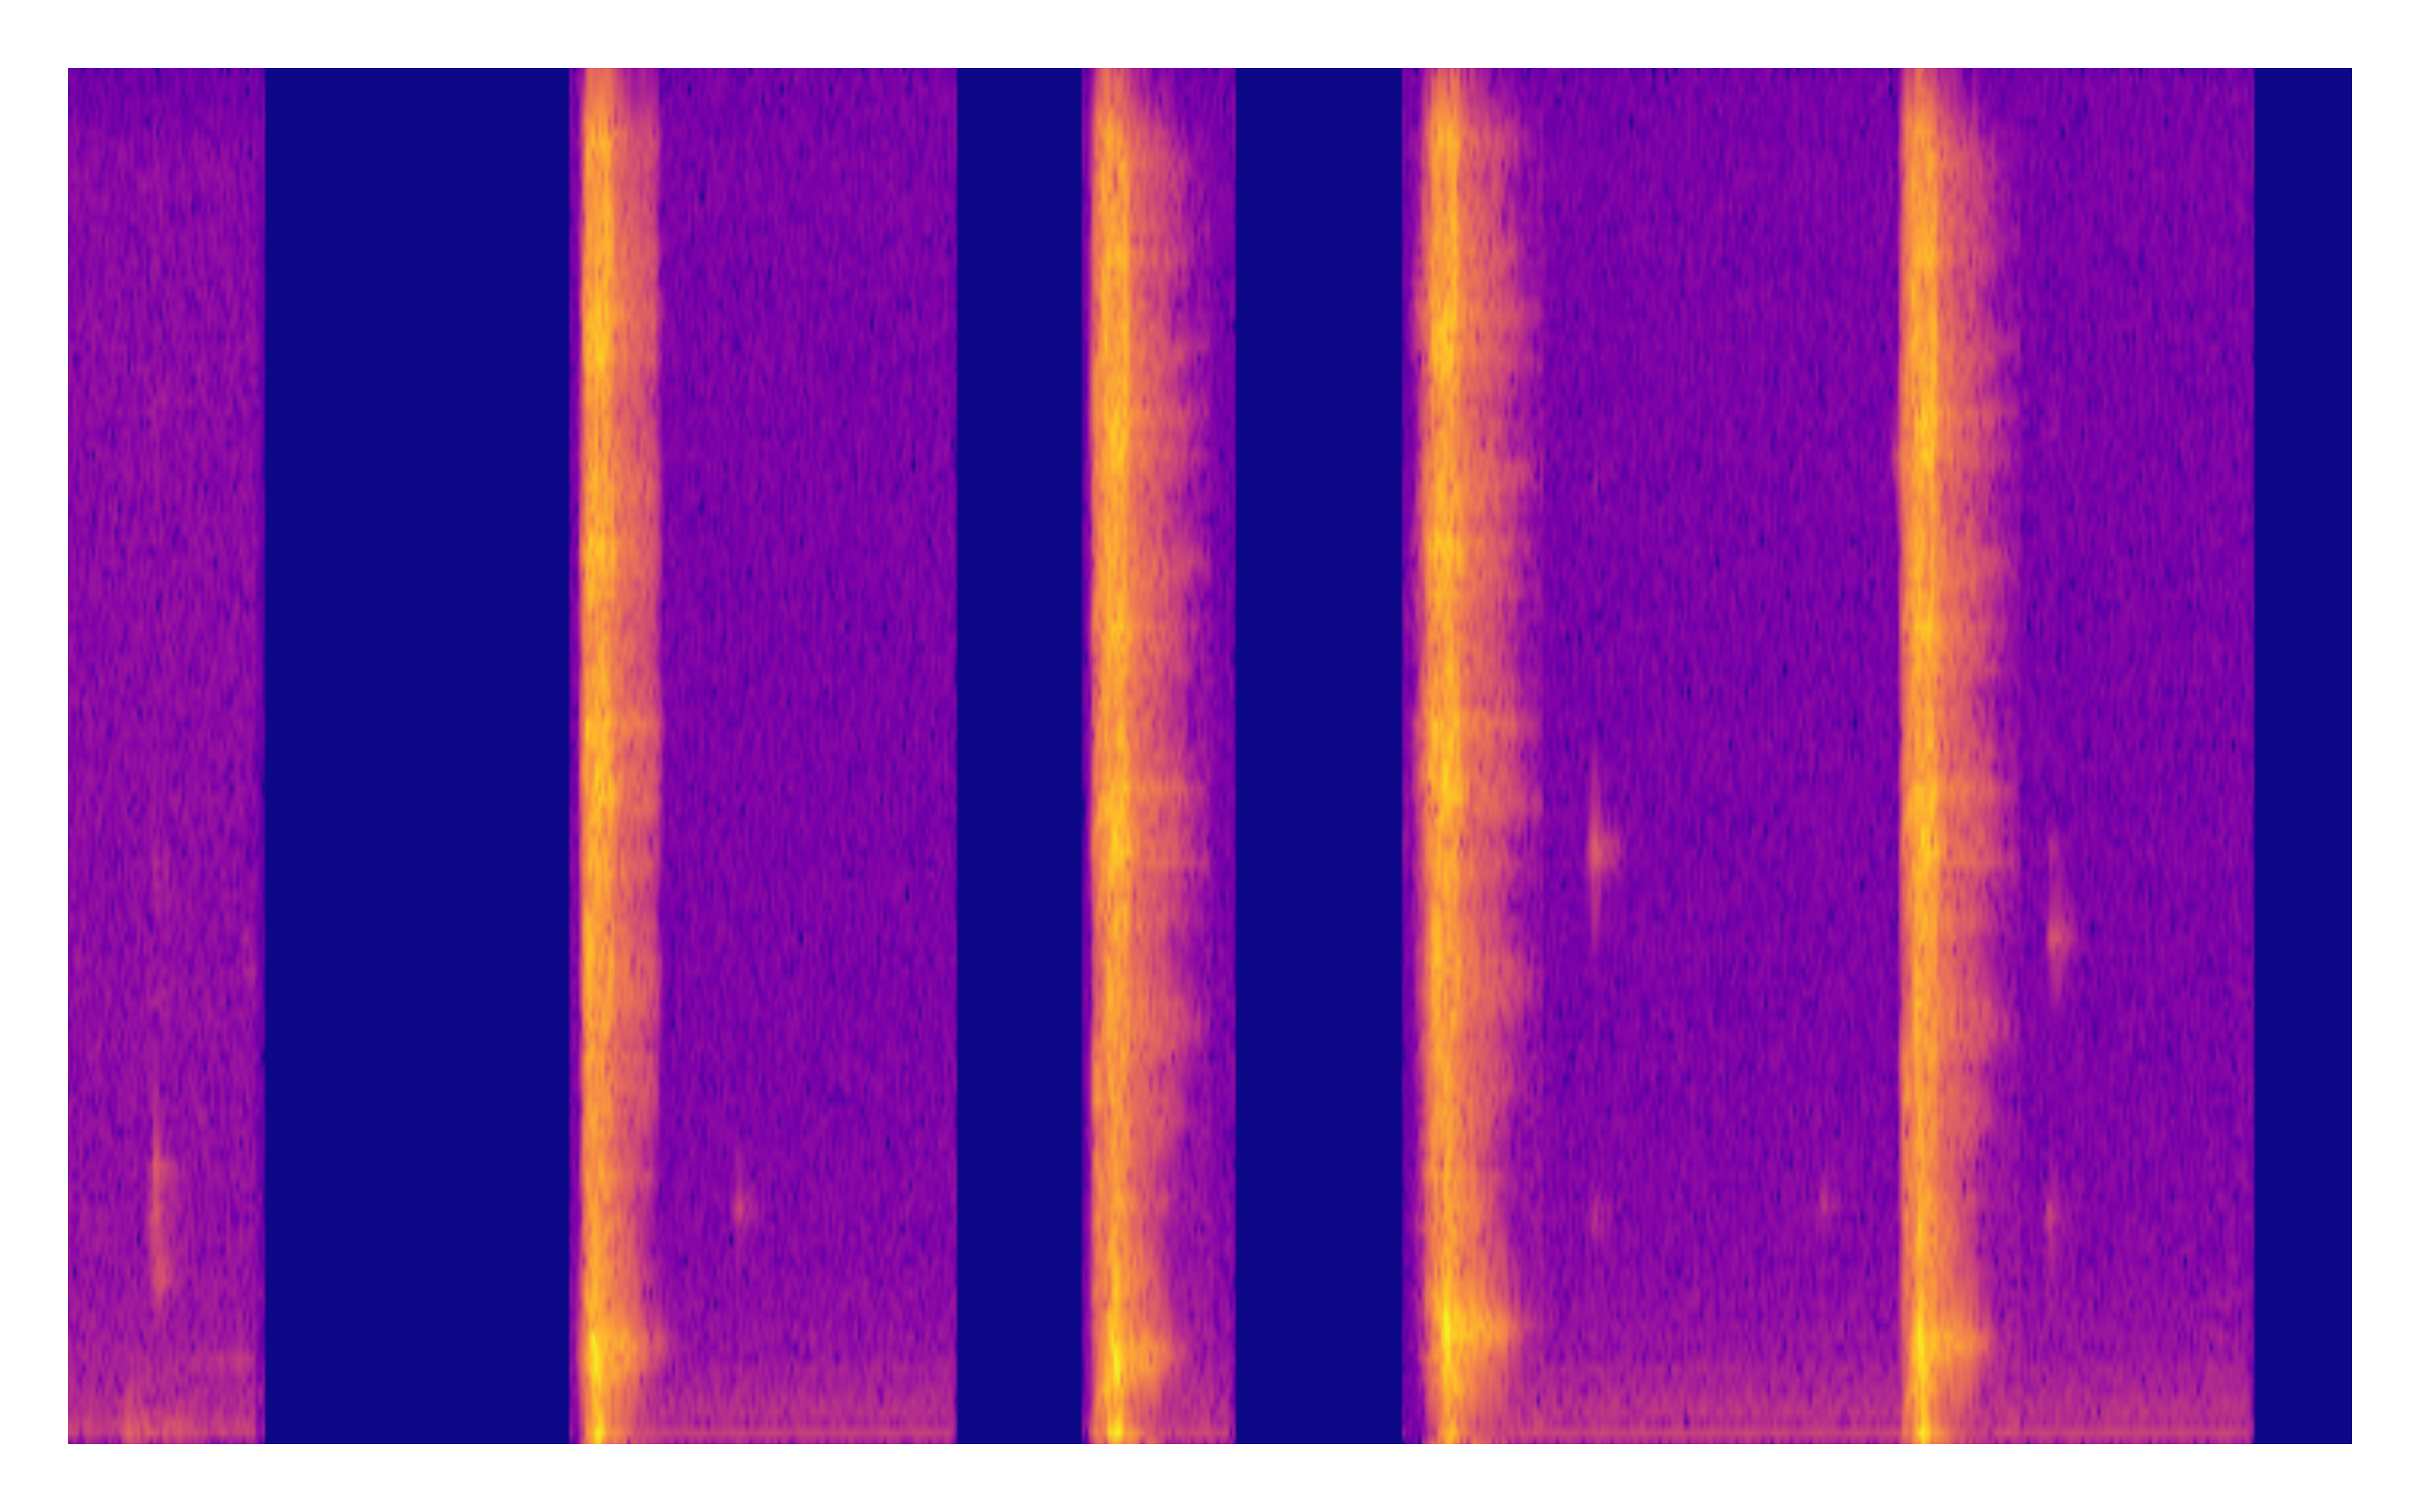
\includegraphics[width=\textwidth]{plots/sword_swoosh/clap target_spectrogram.png}
        \caption*{Target}
    \end{subfigure}
     \begin{subfigure}[b]{0.3\textwidth}
        \centering
        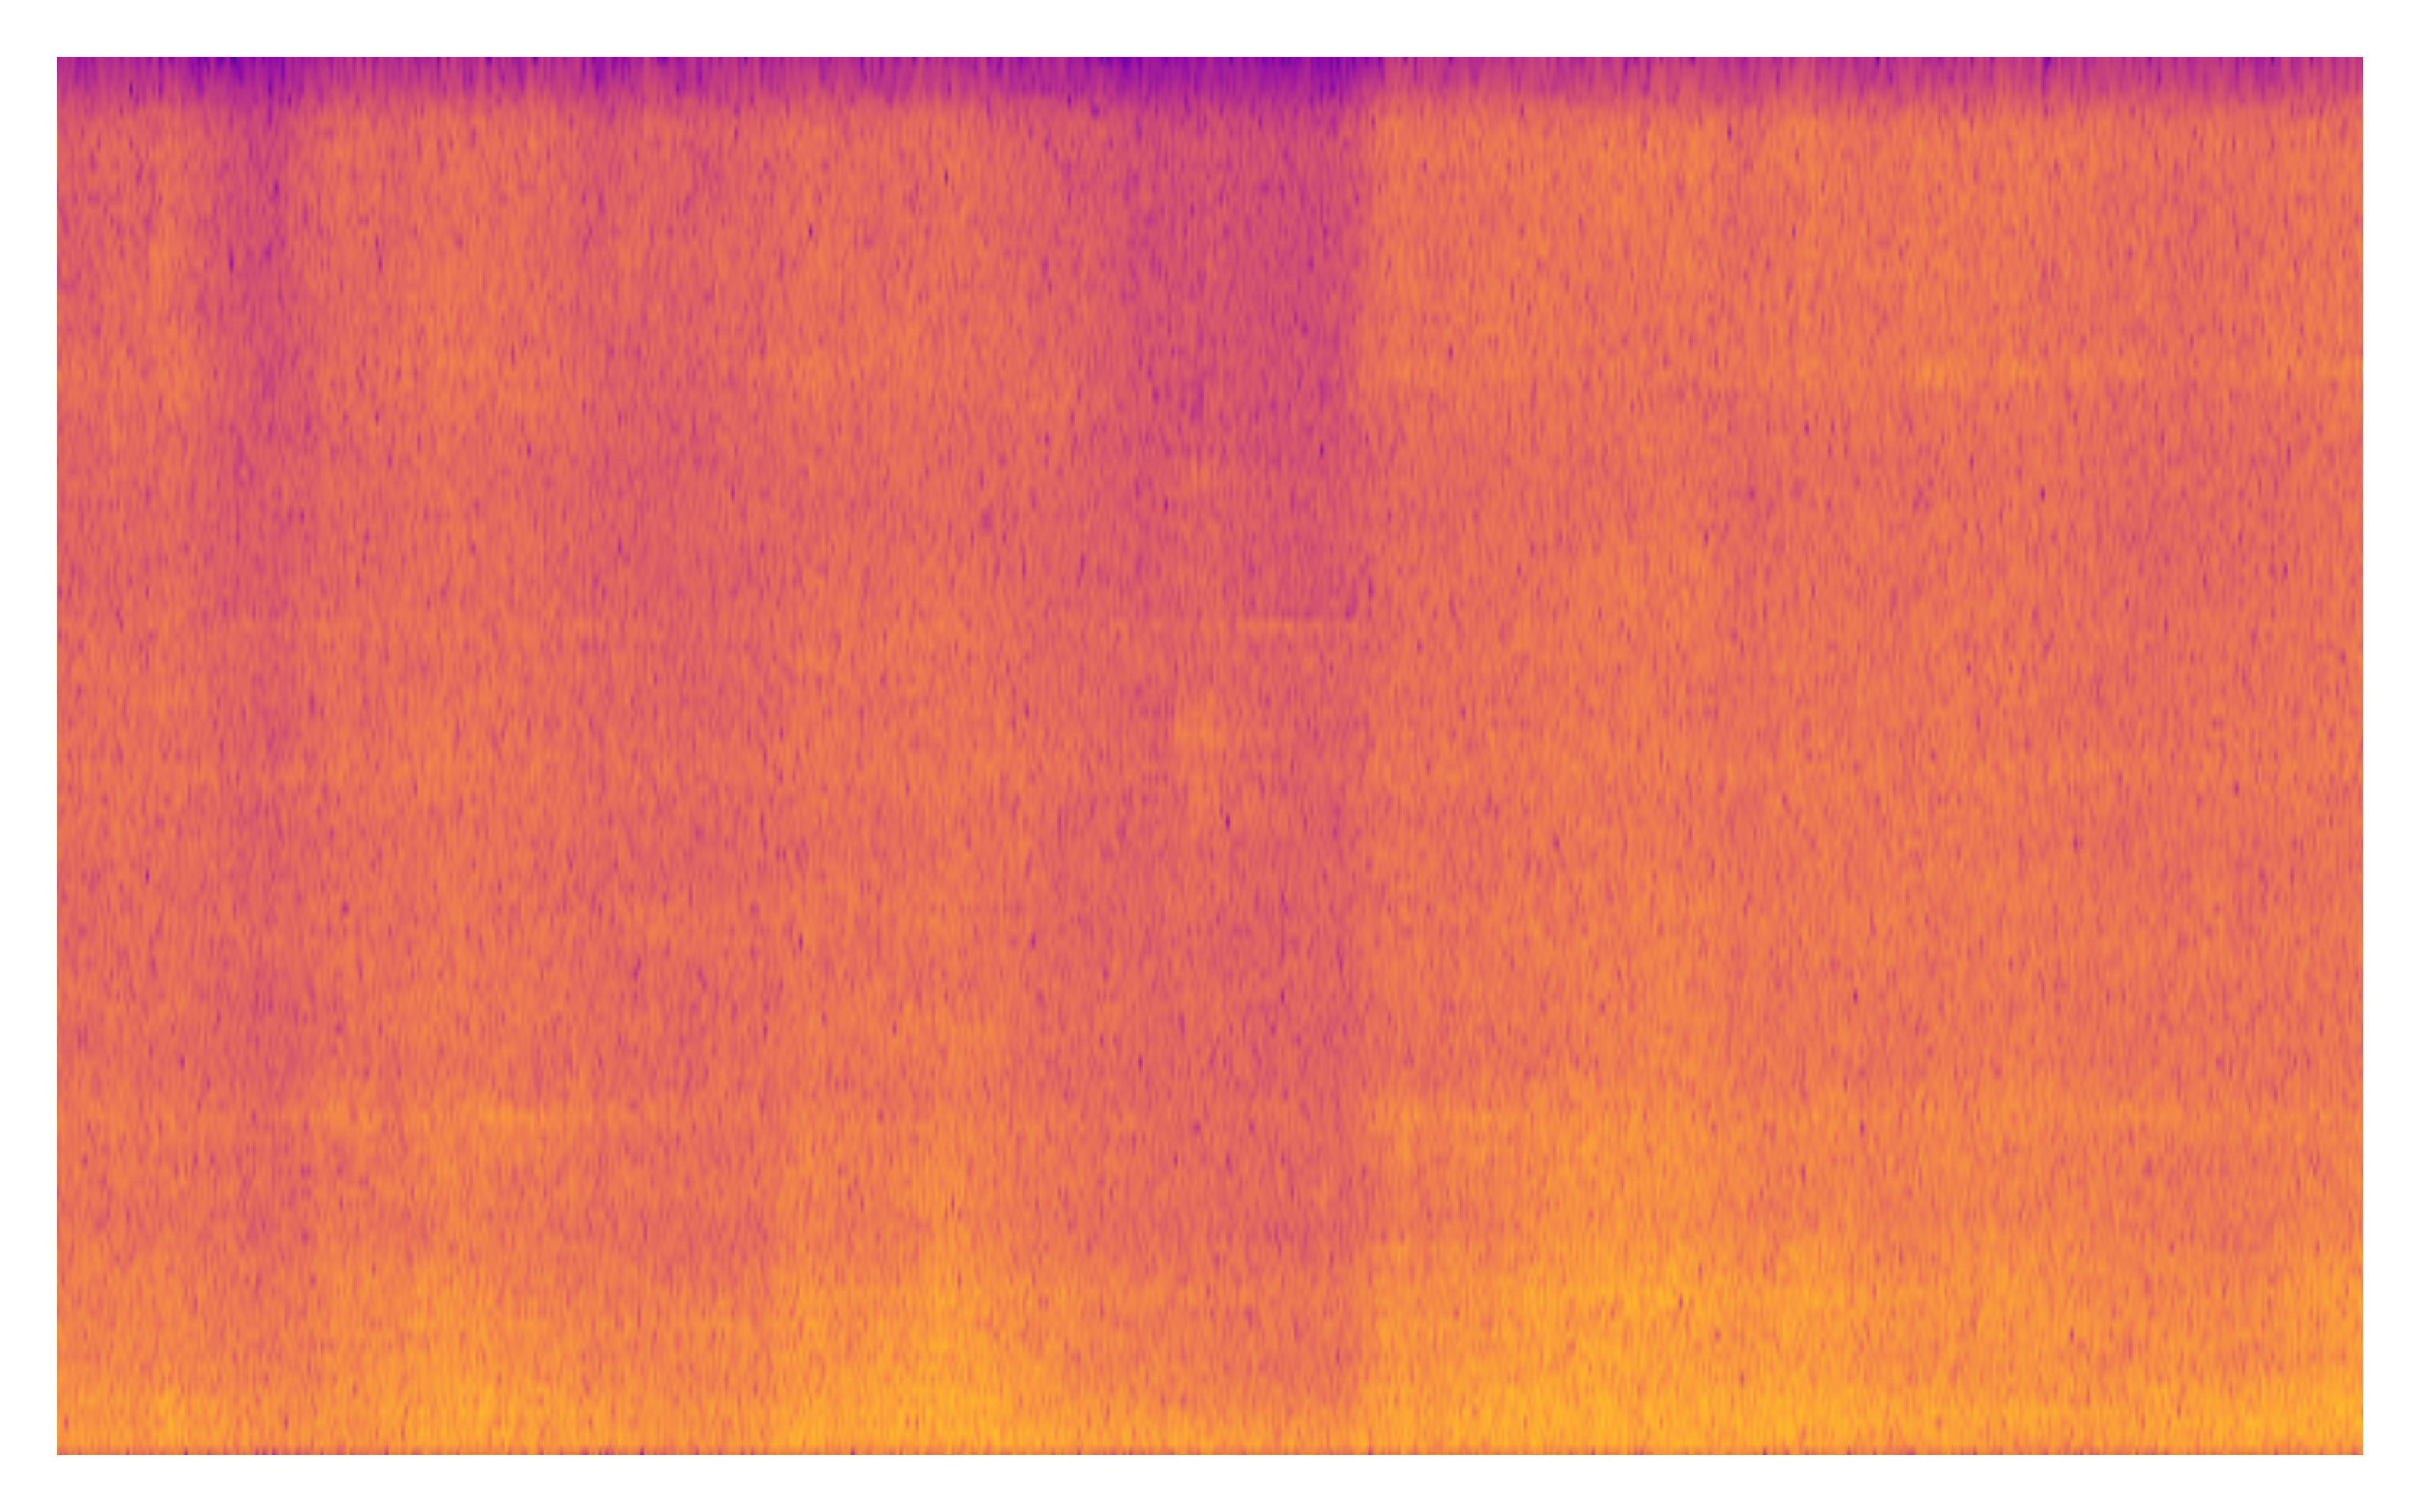
\includegraphics[width=\textwidth]{plots/sword_swoosh/clap noise_spectrogram.png}
        \caption*{Noise}
    \end{subfigure}

    % Row: Original caption, ONE-PEACE sep, CLAP sep
    \begin{subfigure}[b]{0.3\textwidth}
        \centering
        \scriptsize\textbf{"The sword swooshes through the air as someone waves it, making a whooshing sound"}
        \vspace{10mm}
    \end{subfigure}
    \begin{subfigure}[b]{0.3\textwidth}
        \centering
        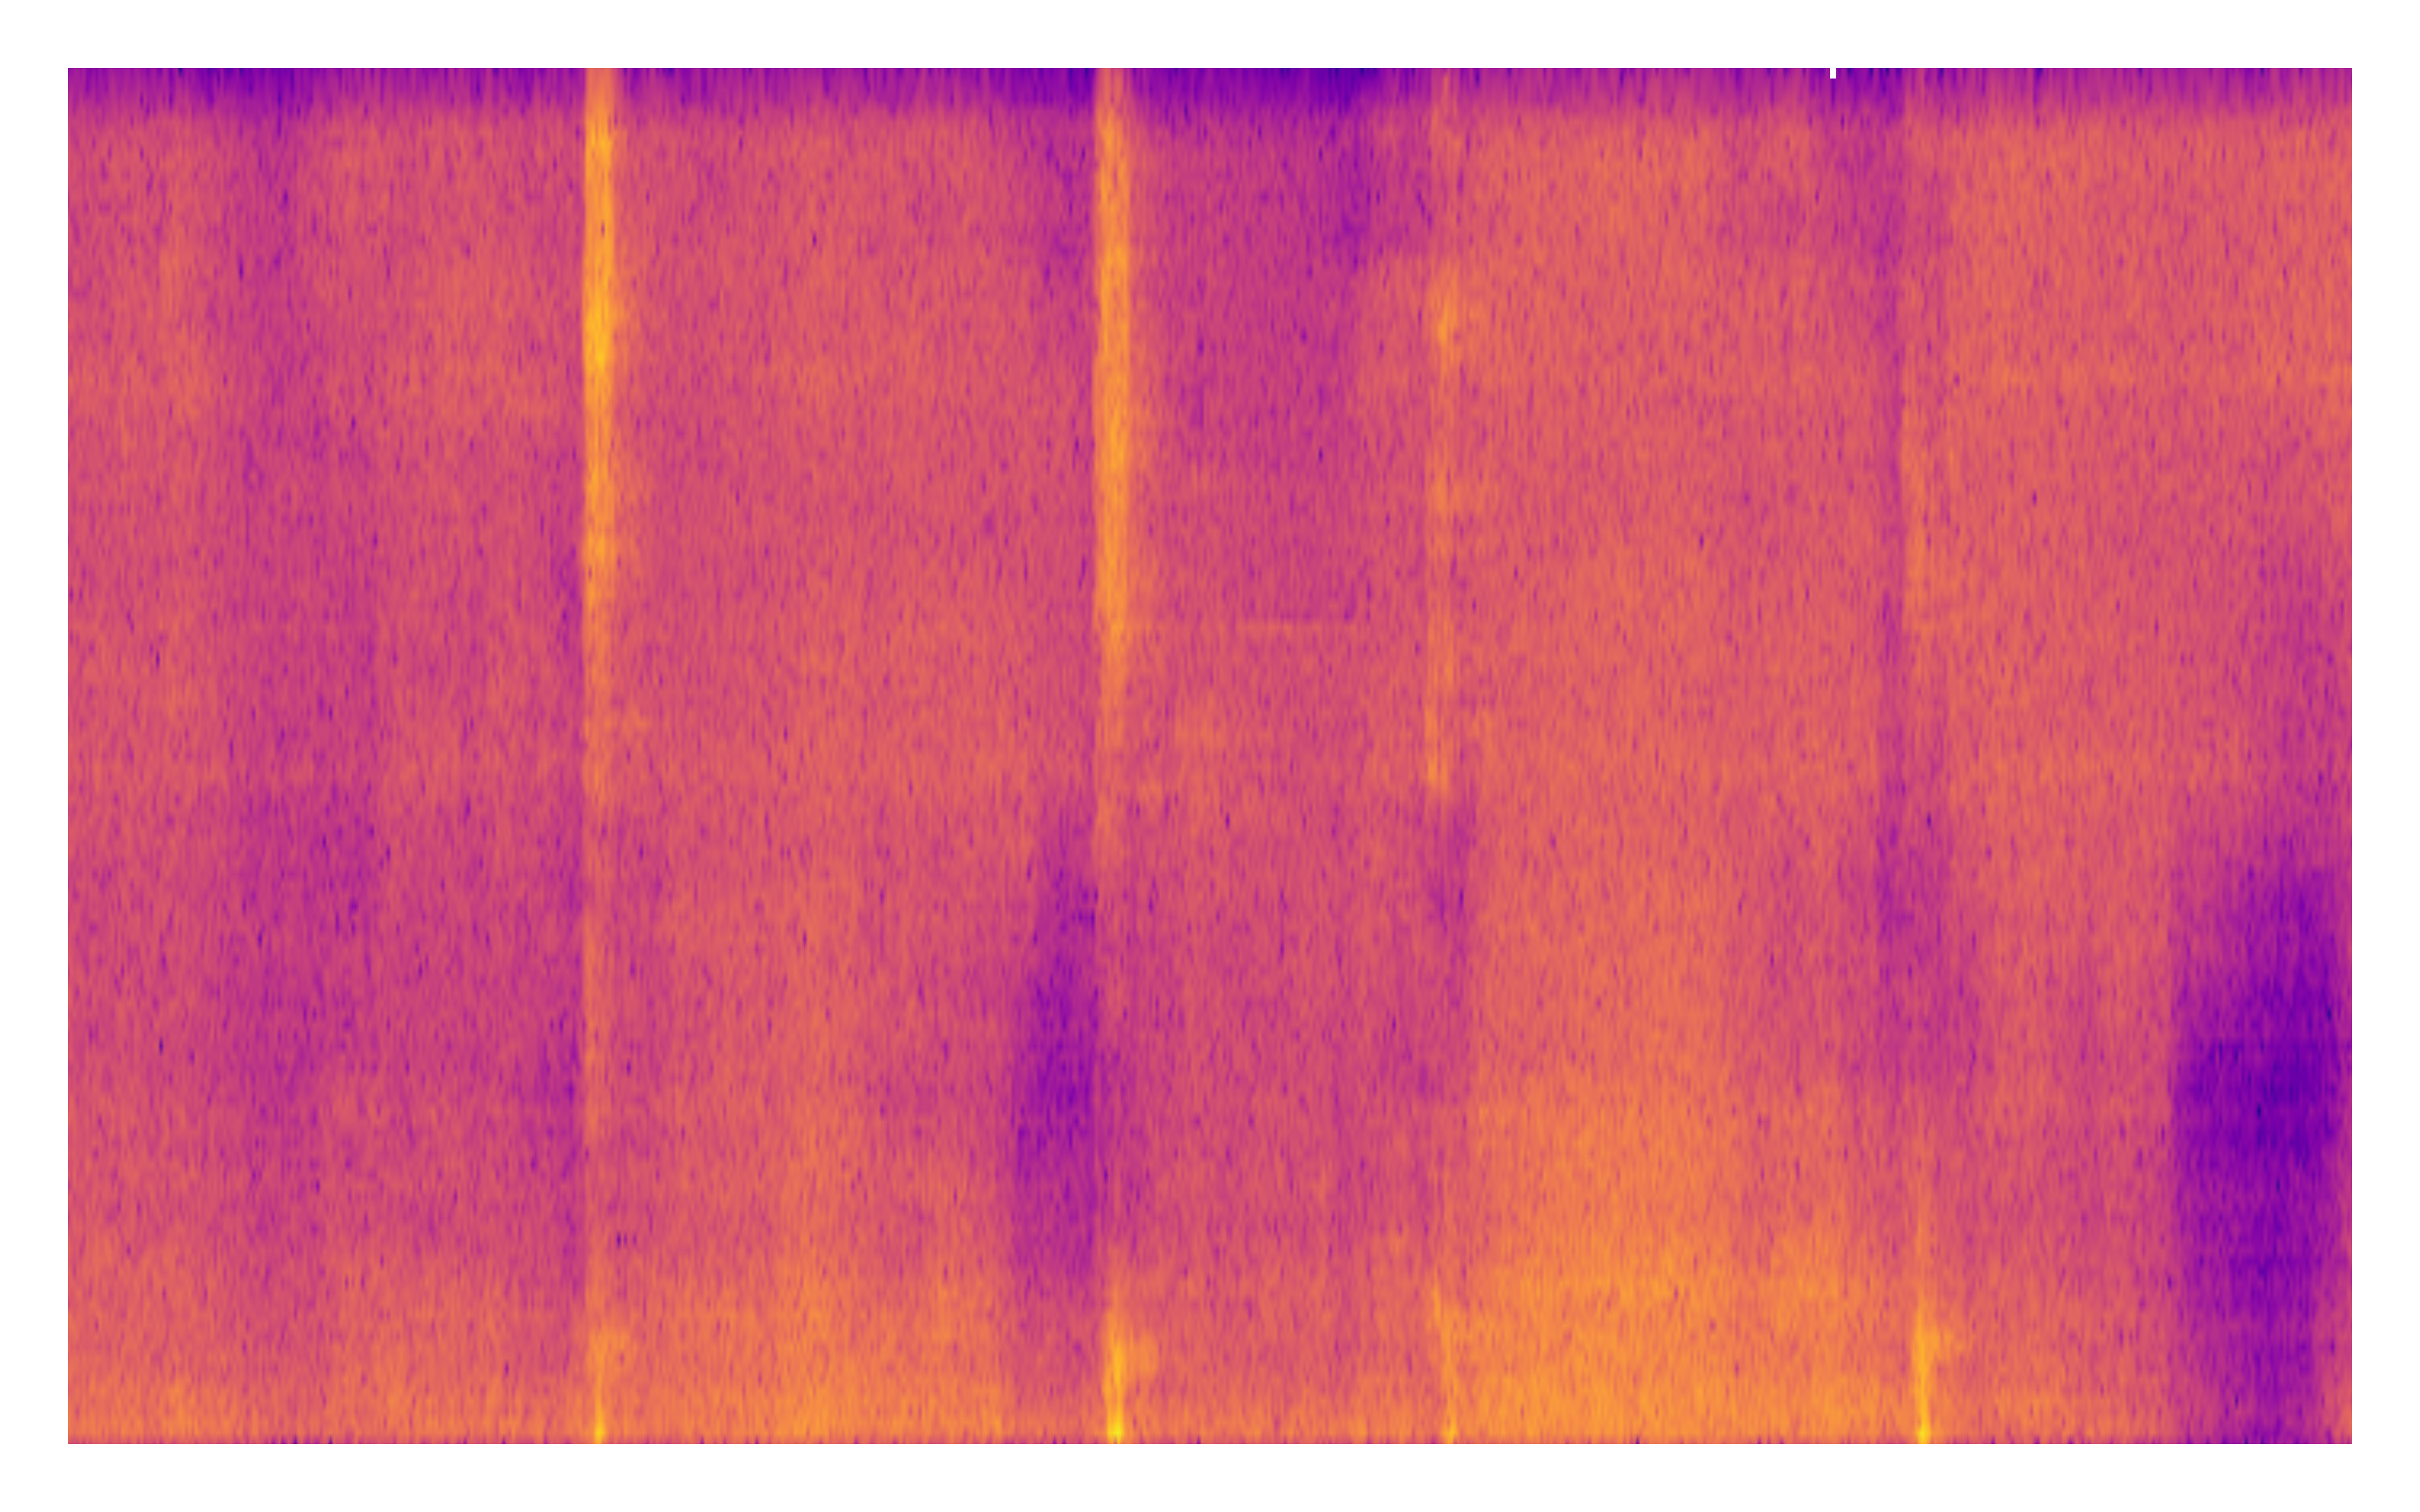
\includegraphics[width=\textwidth]{plots/sword_swoosh/onepeace sep_spectrogram.png}
    \end{subfigure}
    \begin{subfigure}[b]{0.3\textwidth}
        \centering
        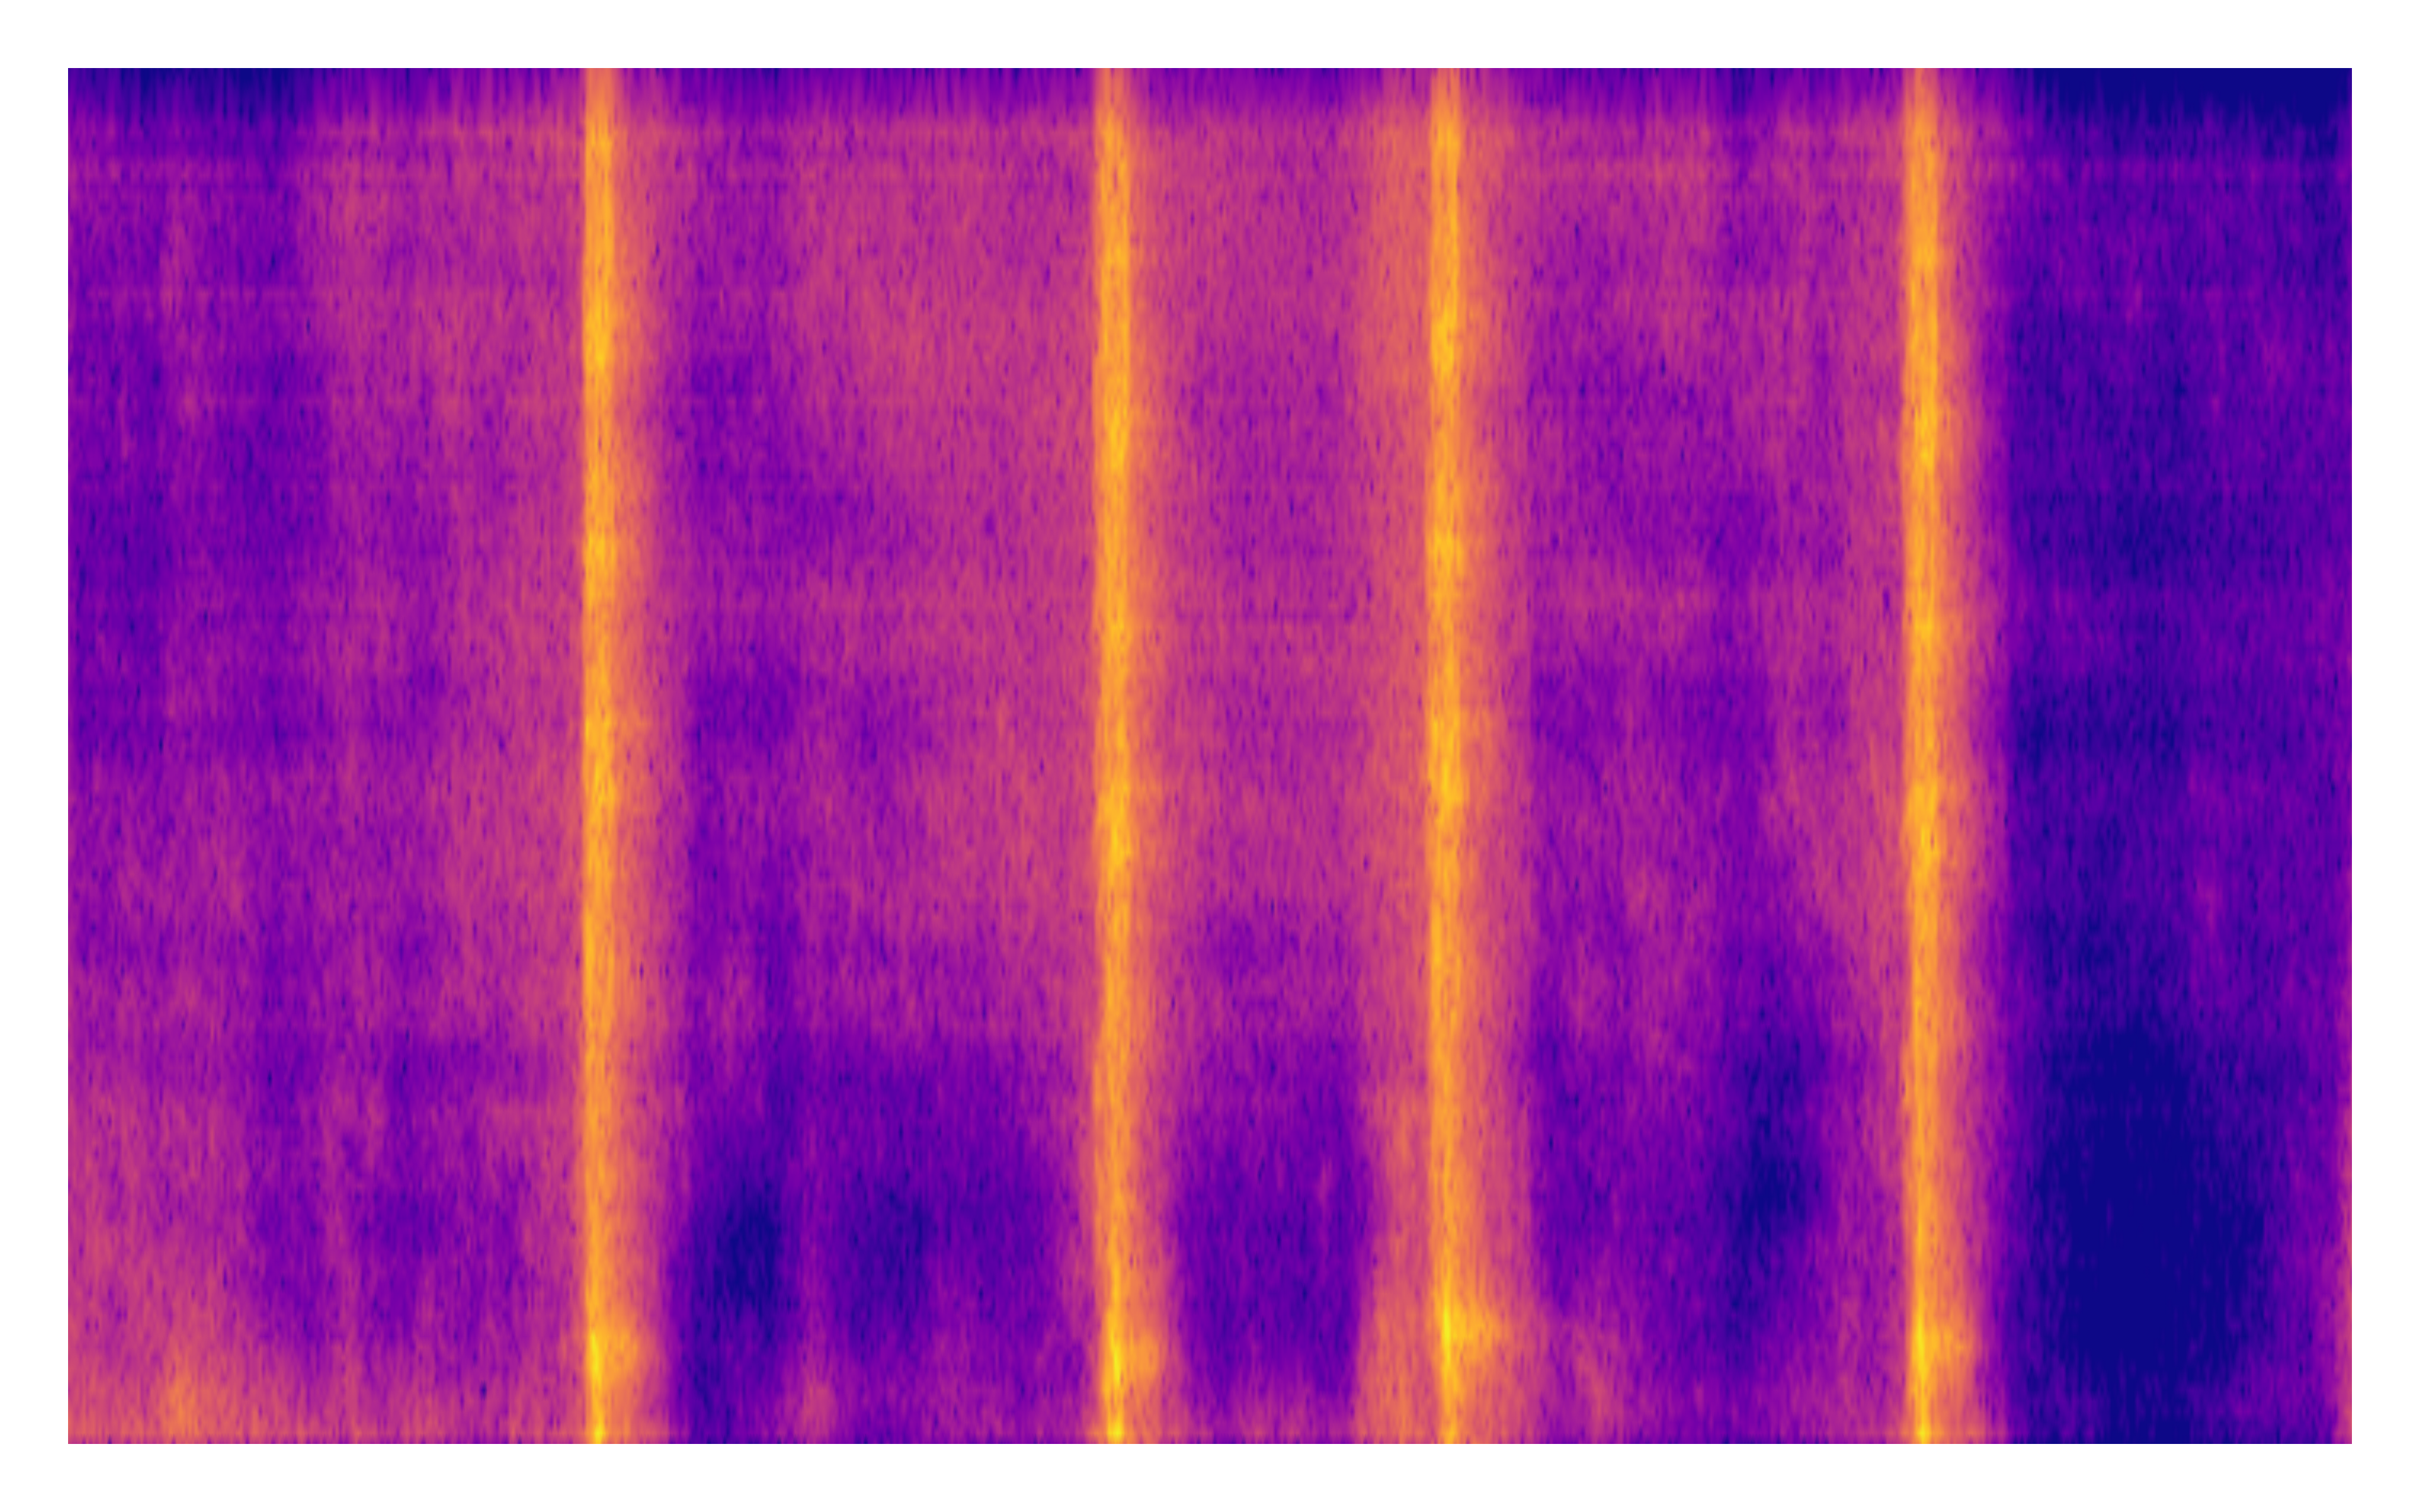
\includegraphics[width=\textwidth]{plots/sword_swoosh/clap sep_spectrogram.png}
    \end{subfigure}

    % Row: Caption#0, ONE-PEACE sep, CLAP sep
    \begin{subfigure}[b]{0.3\textwidth}
        \centering
        \scriptsize\textbf{"The sword slashes through the air"}
        \vspace{13mm}
    \end{subfigure}
    \begin{subfigure}[b]{0.3\textwidth}
        \centering
        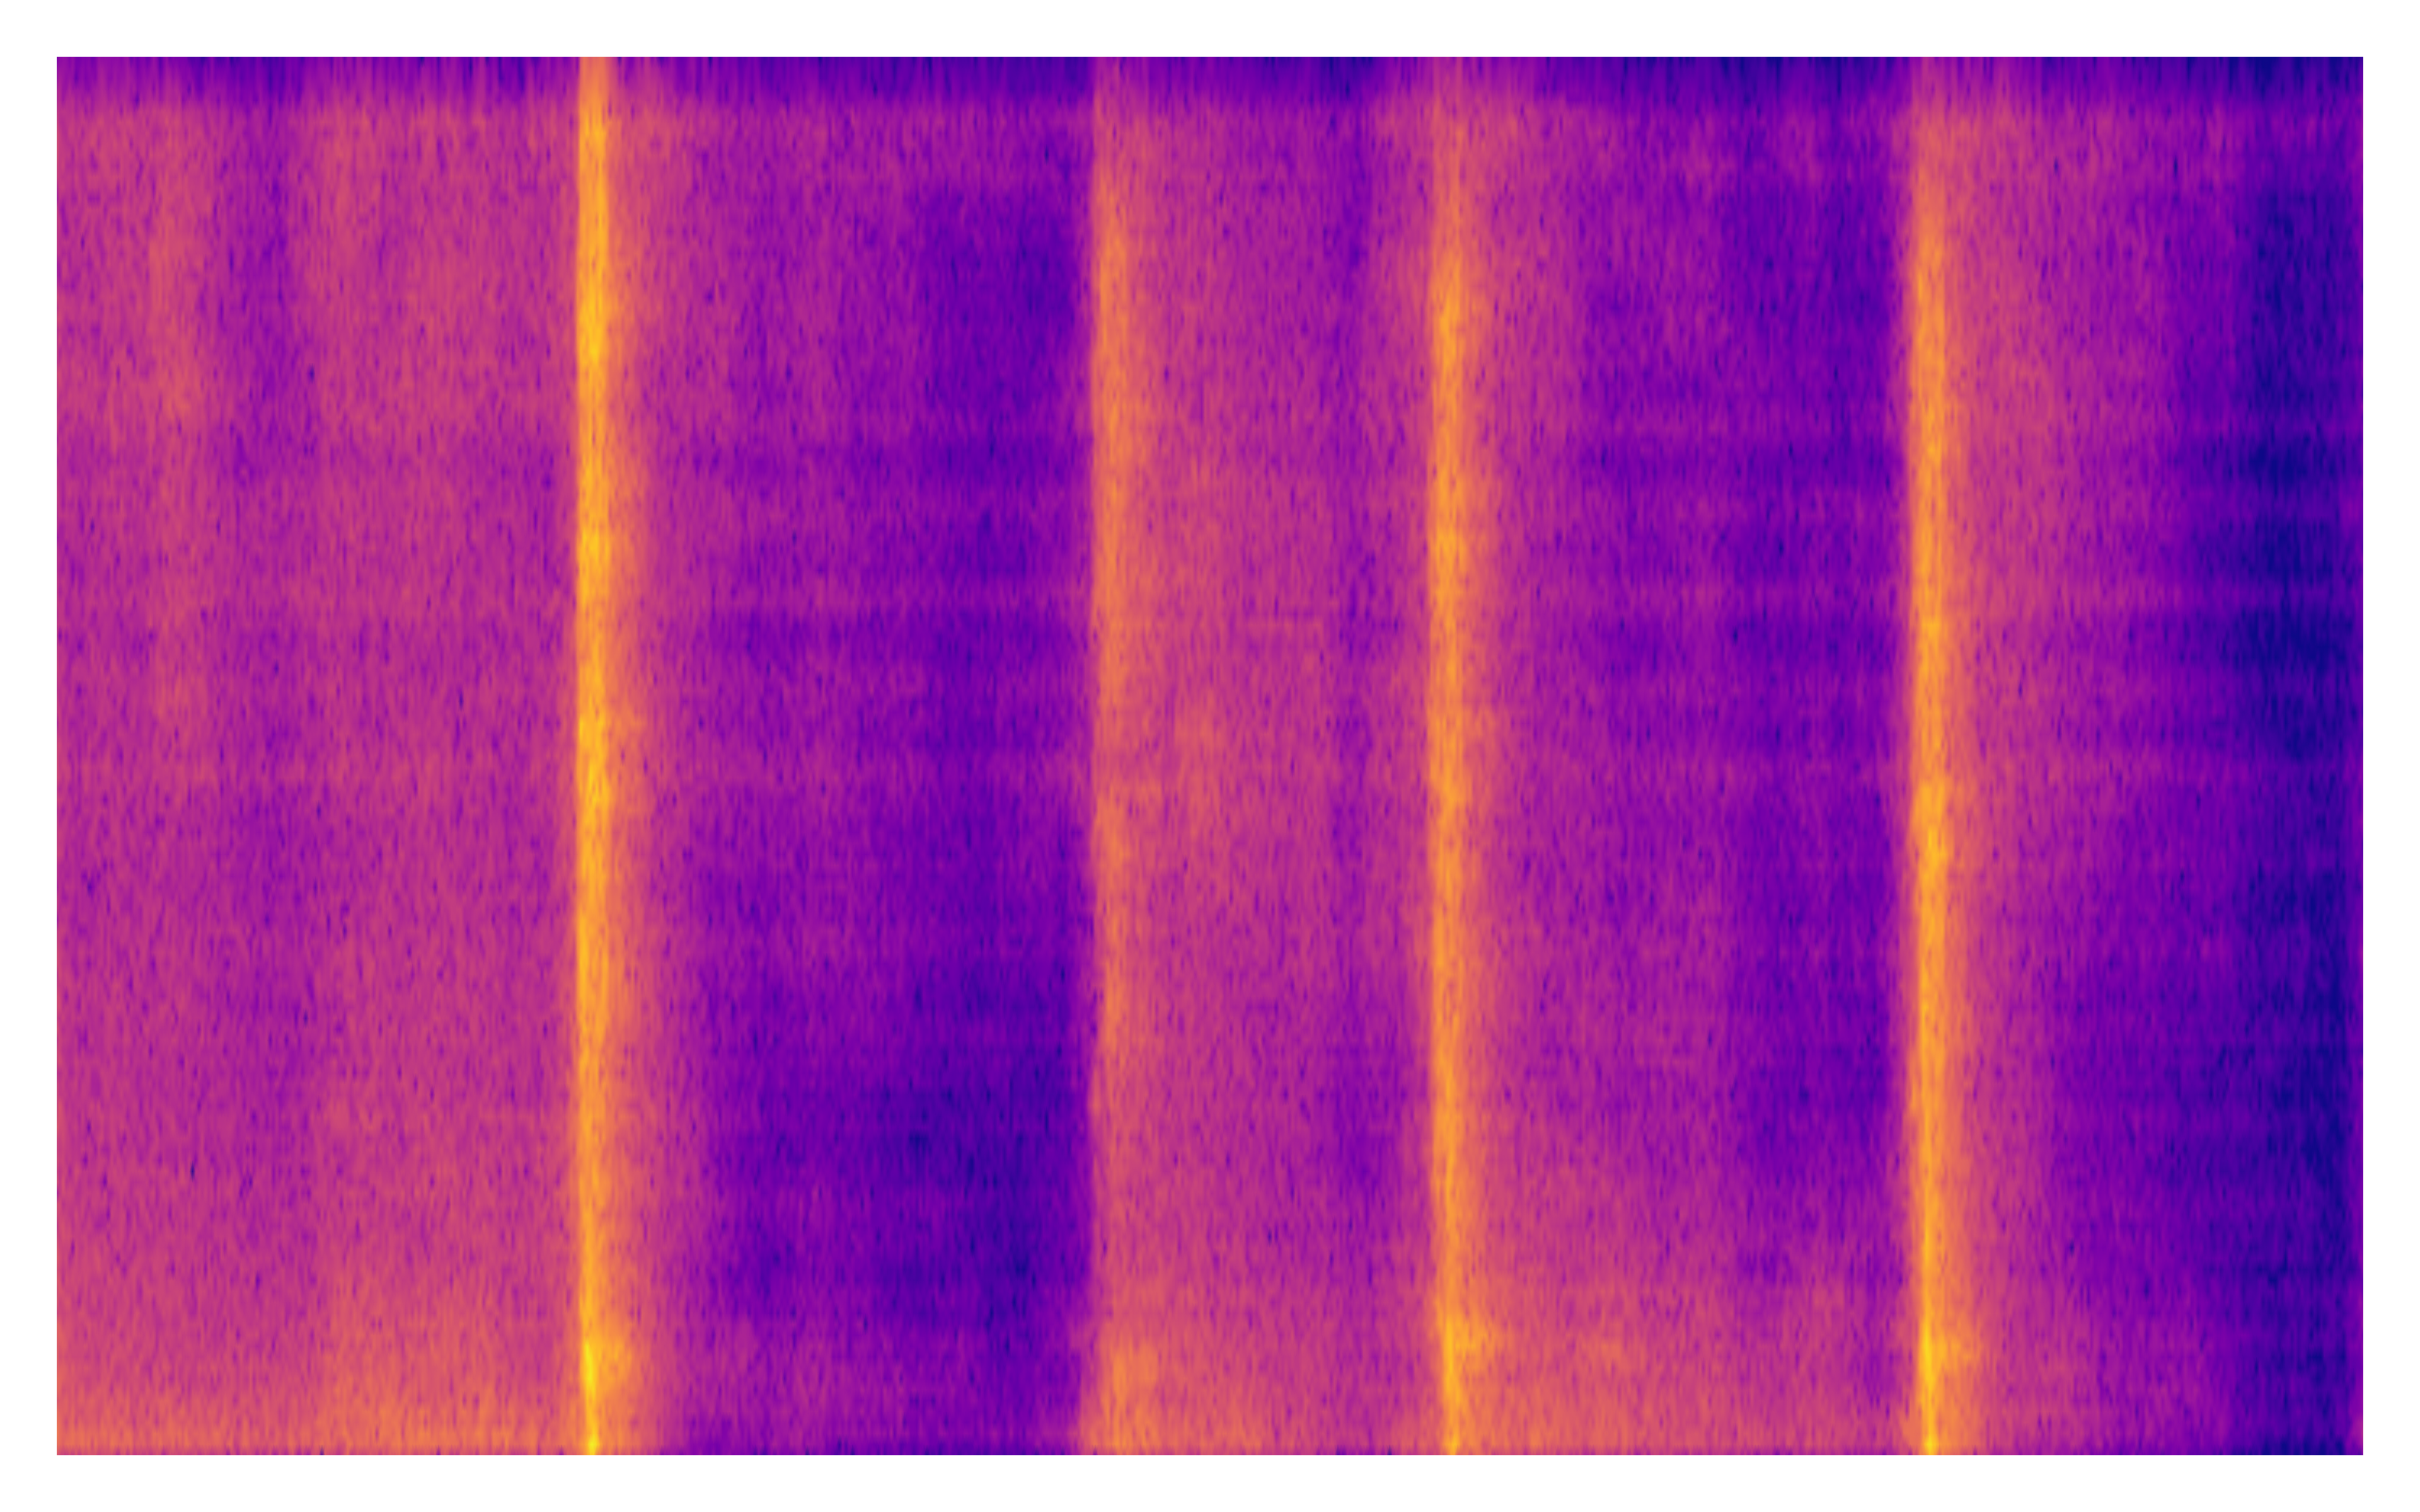
\includegraphics[width=\textwidth]{plots/sword_wave_0/onepeace sep_spectrogram.png}
    \end{subfigure}
    \begin{subfigure}[b]{0.3\textwidth}
        \centering
        \includegraphics[width=\textwidth]{plots/sword_wave_0/clap sep_spectrogram.png}
    \end{subfigure}

    % Row: Caption#2, ONE-PEACE sep, CLAP sep
    \begin{subfigure}[b]{0.3\textwidth}
        \centering
        \scriptsize\textbf{"The sword slices through the air"}
        \vspace{13mm}
    \end{subfigure}
    \begin{subfigure}[b]{0.3\textwidth}
        \centering
        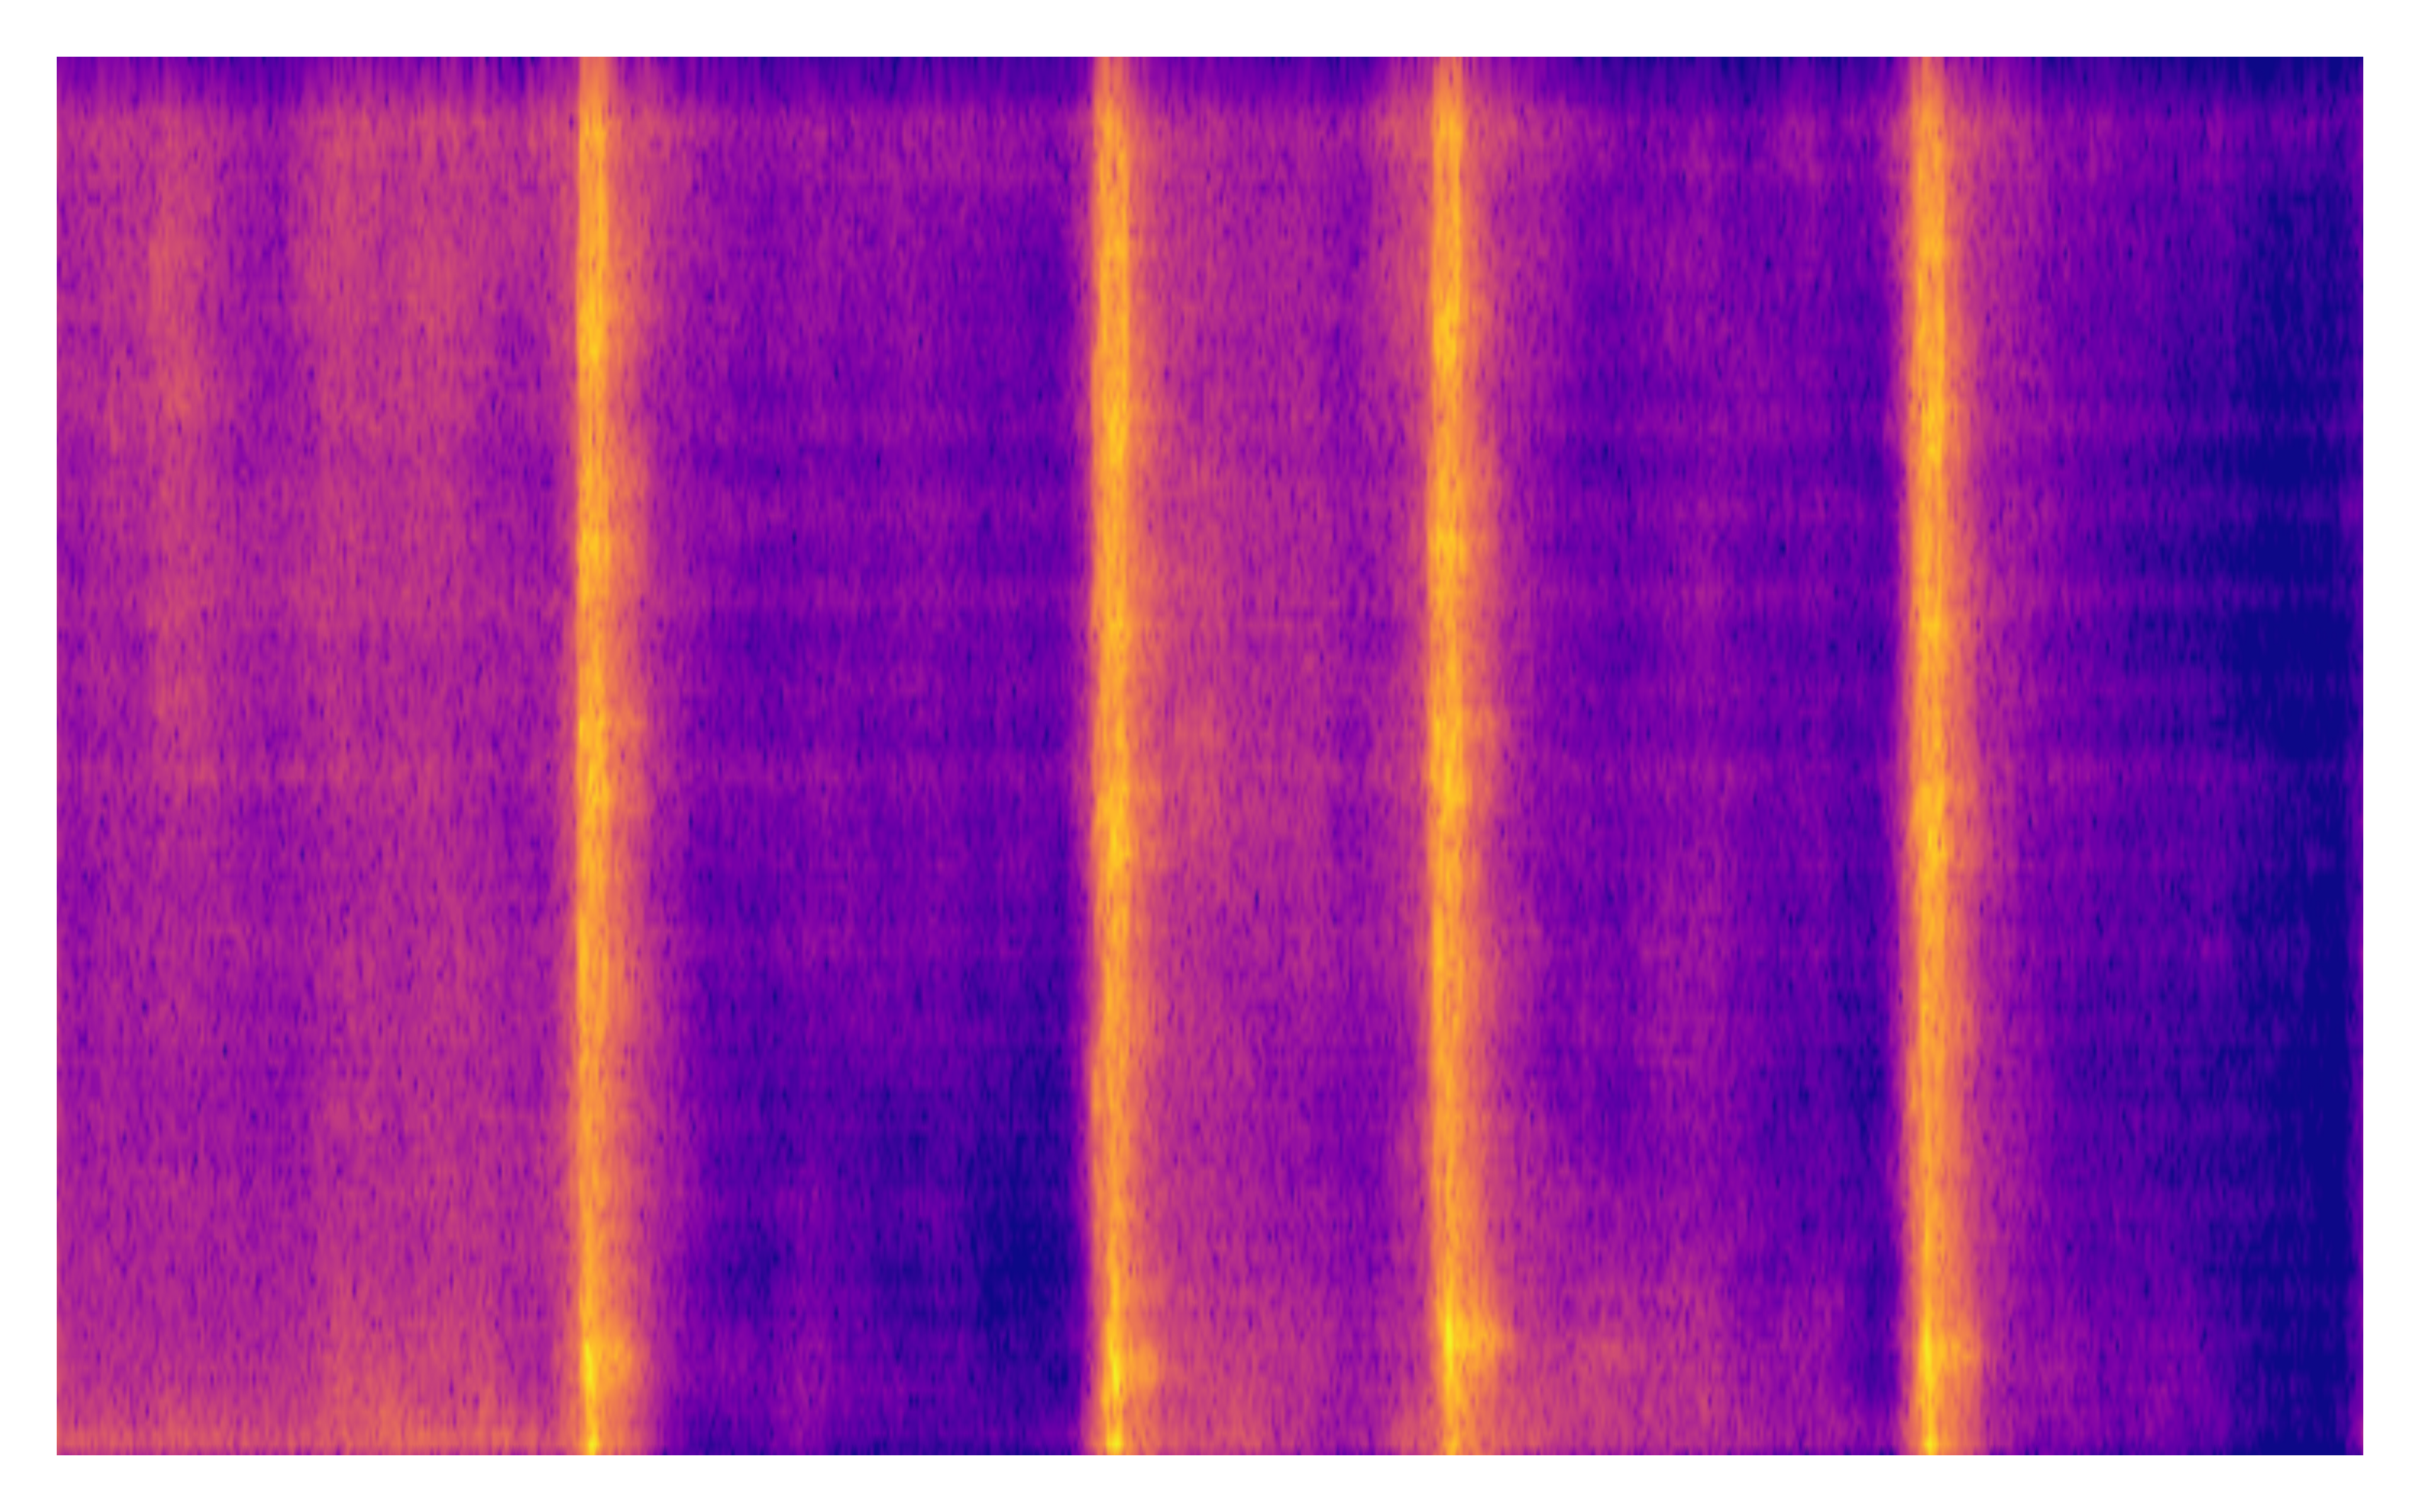
\includegraphics[width=\textwidth]{plots/sword_wave_1/onepeace sep_spectrogram.png}
    \end{subfigure}
    \begin{subfigure}[b]{0.3\textwidth}
        \centering
        \includegraphics[width=\textwidth]{plots/sword_wave_1/clap sep_spectrogram.png}
    \end{subfigure}

    % Row: Caption#1, ONE-PEACE sep, CLAP sep
    \begin{subfigure}[b]{0.3\textwidth}
        \centering
        \scriptsize\textbf{"The waving sword waves around wavily"}
        \vspace{13mm}
        \caption*{Caption}
    \end{subfigure}
    \begin{subfigure}[b]{0.3\textwidth}
        \centering
        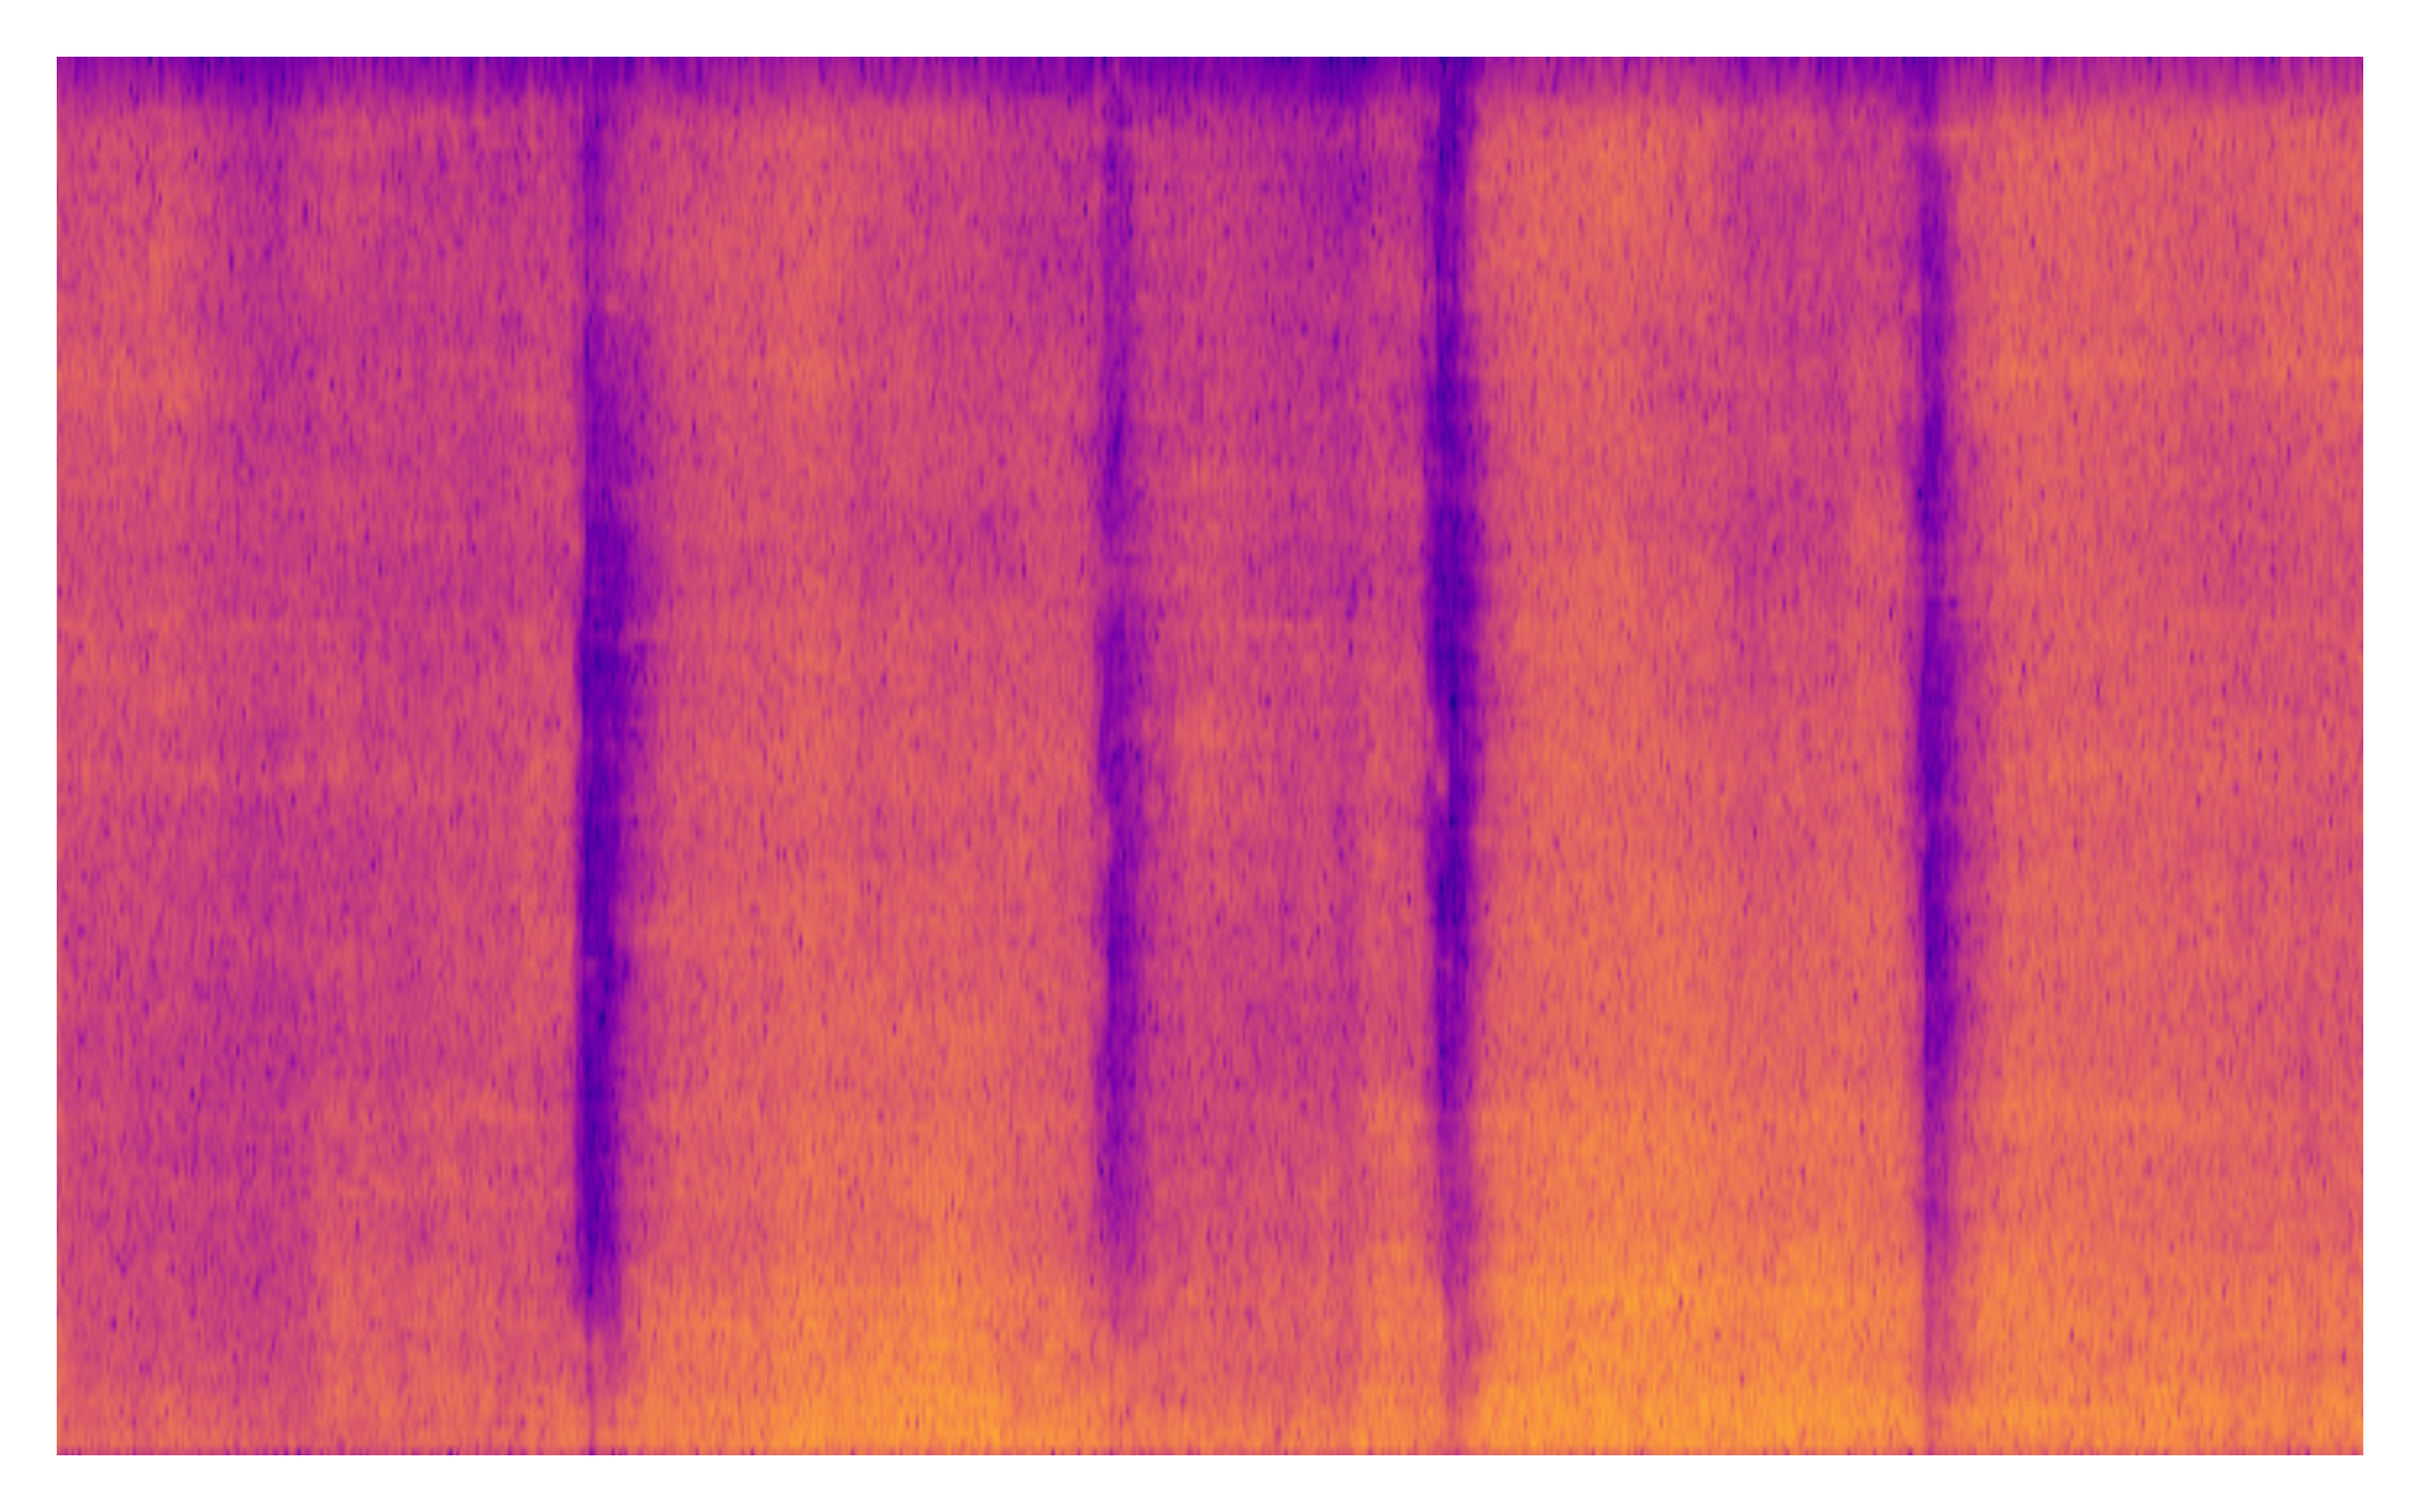
\includegraphics[width=\textwidth]{plots/sword_wave_2/onepeace sep_spectrogram.png}
        \caption*{ONE-PEACE}
    \end{subfigure}
    \begin{subfigure}[b]{0.3\textwidth}
        \centering
        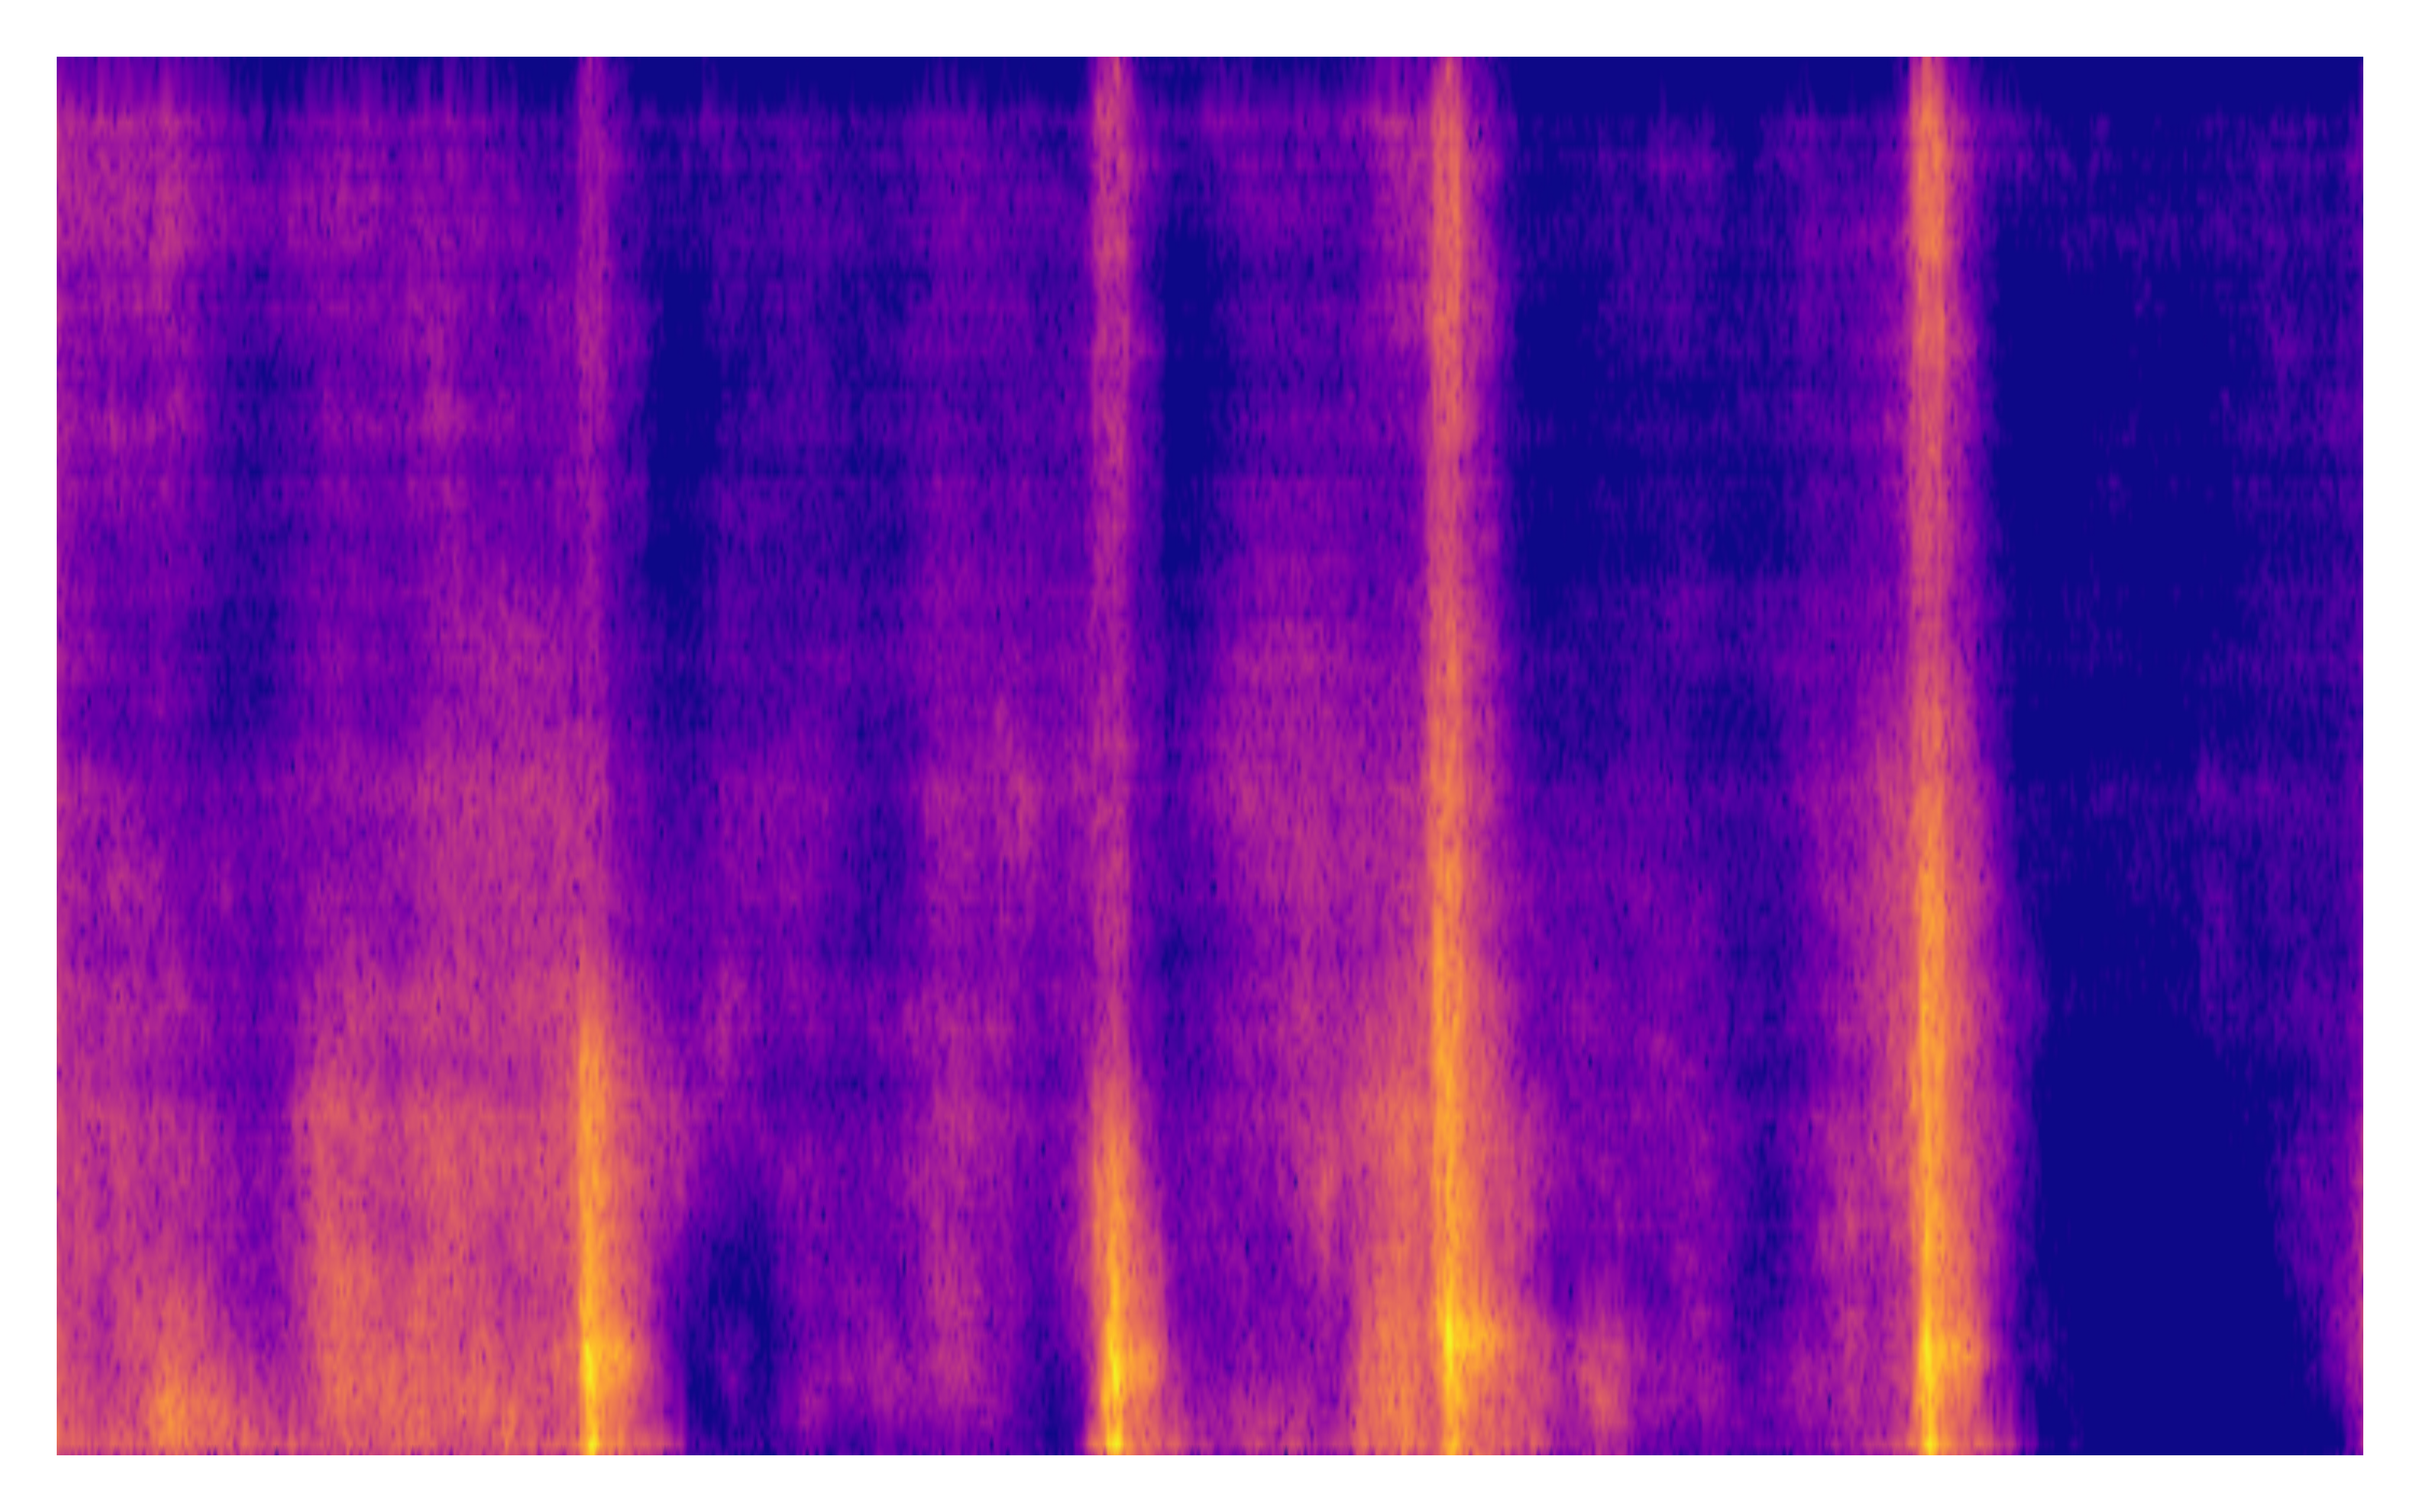
\includegraphics[width=\textwidth]{plots/sword_wave_2/clap sep_spectrogram.png}
        \caption*{CLAP}
    \end{subfigure}
    
    % Continue rows similarly for other queries
    % Add caption below
    \caption{Visualized spectrograms for prompt engineering experiment. Small changes to the text prompt drastically effect the audio output when using ONE-PEACE.}
    
    \label{fig:separation_results}

\end{figure*}

\label{fig:sword_spectrograms}

\begin{figure*}[!htbp]

    \begin{subfigure}[b]{0.5\textwidth}
        \centering
        \includegraphics[width=\textwidth]{plots/similarity_vs_sdr/baseline_deltasim_sdri.png}
        \caption*{CLAP}
    \end{subfigure}
    \begin{subfigure}[b]{0.5\textwidth}
        \centering
        \includegraphics[width=\textwidth]{{plots/similarity_vs_sdr/onepeace_deltasim_sdri.png}}
        \caption*{ONE-PEACE}
    \end{subfigure}
    
    \caption{Comparison between improvement in SDR and increase in embedded similarity between input and output audio files. Neither CLAP nor ONE-PEACE show much noticeable correlation between SDR and similarity.}
    
    \label{fig:sdr_vs_sim}

\end{figure*}


\section{Analysis}

\subsection{Vector Similarity}

In service of understanding the impact of the different embeddings on the AudioSep model's ability to understand the input text prompt, we measured the cosine similarity between audio files and the text prompt in the embedding space. Figure~\ref{fig:sdr_vs_sim} shows a comparison between SDRi and the change in similarity in both CLAP and ONE-PEACE. Each point is a unique input, with its horizontal position indicating the change in cosine similarity between the input and output audio files, and its vertical position indicating the change in SDR between the input and output audio files.

The plots indicate little to no correlation between the change in similarity and the improvement in SDR. This suggests that the model does not work by merely trying to generate audio that is closer to the text prompt in the embedding space. It appears that instead of specific differences in the alignment of the their encoders, the performance disparity between the two models is better explained by structural details such as the type/amount of information encoded by the text encoders or patterns in the descriptiveness of the human-produced captions which may lead to overfitting.

\subsection{Prompt Engineering}

When looking for outlier test cases, we found several where ONE-PEACE performed significantly worse than CLAP. We noticed that the several with the highest discrepancy shared a commonality, the presence of the word ``whoosh'' in the prompt. In all cases, ONE-PEACE preserved significant parts of the noise audio, which were soft whitenoise compared to the relatively sharp source audio. This suggests that the ONE-PEACE encoding may interpret ``whoosh'' sounds as gradual and drawn-out, leading to it prioritizing much more of the noise.

Figure~\ref{fig:sword_spectrograms} shows one such test case that was especially egregious. SDR and similarity metrics are reported in Table~\ref{tab:sword_clap} and Table~\ref{tab:sword_onepeace}. The prompt in this case was ``The sword swooshes through the air as someone waves it, making a whooshing sound.'' The source audio sounds like multiple quick slashing sounds. The noise audio is annotated ``The engine is accelerating and birds are singing'' but sounds similar to ambient noise of crashing waves. ONE-PEACE seemingly thinks the caption better describes the noise audio than the source audio, because it flattens the sword slashes while keeping the waves. This may be partially due to its interpretation of a whoosh sound. Moreover, this example is amusing because the prompt coincidentally includes the word ``waves'', potentially further confusing the text encoder.

To examine the effect of the prompt on the text encoders, we modified the text prompt slightly to emphasize different aspects of the audio mixture. By changing the sound descriptor from a ``whoosh'' to a ``slice'' or ``slash'', we were able to guide ONE-PEACE to obtain virtually the same SDR achievable by CLAP. On the other hand, by artificially inserting variations of the word ``wave'', we were able to trick ONE-PEACE into keeping only the noise and masking away all of the source audio. On the other hand, CLAP is mostly unaffected by these changes in word choice. This suggests differences between the sensitivity of ONE-PEACE and CLAP to various parts of the text prompt. Whereas ONE-PEACE takes into account the entirety of the prompt (allowing us to mislead it by filling the sentence with distracting words), CLAP may fixate on the main subject of the prompt, ``sword'', which is the invariant in these different prompts. This could be due to the higher dimensionality of the ONE-PEACE encoding or differences in the attention layers of the two encoders. Regardless, this implies that one way to improve the performance of ONE-PEACE is by increasing the specificity of the text prompts.



% Prompt engineering metrics table CLAP
\begin{table*}[!htbp]
  \centering

  \small
  \begin{tabular}{ccccccc}
    \textbf{Caption}    & \textbf{SDR}  & \textbf{SDRi} & \textbf{SI-SDR}  & \textbf{I-Similarity}  & \textbf{O-Similarity} & \textbf{T-Similarity} \\
    \hline
    
    \makecell{``The sword swooshes through the air \\ as someone waves it, making \\ a whooshing sound''\\}  & 28.56 & 13.56 & 28.56 & 0.3910 & 0.56039 & 0.3782 \\
    \hline
    \makecell{``The sword slashes through the air''}    & 27.94 & 12.94 & 28.02 & 0.3072 & 0.3132 & 0.3050 \\
    \hline
    \makecell{``The sword slices through the air''}     & 28.39  & 13.39 & 28.42 & 0.2943 & 0.2907 & 0.2556 \\
    \hline
    \makecell{``The waving sword waves around wavily''} & 6.68   & -8.32 & 5.63  & 0.2380 & 0.2189 & 0.1124  \\
    
    \hline
  \end{tabular}
  \caption{CLAP performance metrics on prompt engineering experiment, The similarity metrics refer to cosine similarity between the embedding for the caption and the input mixture (I), output separation result (O), and the target (source) audio (T).}
  
\end{table*}\label{tab:sword_clap}

% Prompt engineering metrics table ONE-PEACE
\begin{table*}[!htbp]
  \centering
  \small
  \begin{tabular}{ccccccc}
    \textbf{Caption}    & \textbf{SDR}  & \textbf{SDRi} & \textbf{SI-SDR}  & \textbf{I-Similarity}  & \textbf{O-Similarity} & \textbf{T-Similarity} \\
    \hline
    
    \makecell{``The sword swooshes through the air \\ as someone waves it, making \\ a whooshing sound''}  & 2.02 & -12.98 & -1.72 & 0.1639 & 0.3155 & 0.3884 \\
    \hline
    \makecell{``The sword slashes through the air''}    & 3.22 & -11.78 & 0.86 & 0.1617 & 0.4141 & 0.3823      \\
    \hline
    \makecell{``The sword slices through the air''}     & 27.10  & 12.10 & 27.27 & 0.2426 & 0.4351 & 0.4560     \\
    \hline
    \makecell{``The waving sword waves around wavily''} & -0.08   & -15.08 &  -39.01 & 0.1584 & 0.1368 & 0.2434  \\
    
    \hline
  \end{tabular}
  
  \caption{ONE-PEACE performance metrics on prompt engineering experiment. The similarity metrics refer to cosine similarity between the embedding for the caption and the input mixture (I), output separation result (O), and the target (source) audio (T).}
  
\end{table*}\label{tab:sword_onepeace}


\paragraph{Contributions}\quad\\
\textbf{Vincent:} training/evaluation of AudioSep models, visualized spectrogram figures, methods+training section and overall paper writing. \\
\textbf{Sambit:} Wrote Section 2, Section 4, Section 5, and part of Introduction. Helped with evaluation metrics and similarities for the validation set. \\
\textbf{Richard:} Analysis and plotting of SDR and cosine similarity, collaboration on prompt engineering, wrote Section 6.

\bibliography{custom}

% \appendix

% \section{Example Appendix}
% \label{sec:appendix}

% This is an appendix.

\end{document}
